% !TeX program = xelatex
% 主编译文件；正文按章节存放在 sections/，全局格式位于 config/preamble.tex。
% 摘要：sections/abstract.tex；一、二问：sections/q1.tex、sections/q2.tex。
% 第三问由 sections/q3.tex 汇总，细分内容见 sections/q3/。
% 文献：references/references.tex；附录：appendices/。
% 编译器使用 XeLaTeX，主文件保持 main.tex；子文件通过 input 引入。
% figures 文件夹保存实机调试照片与各问配图；q1_case.tex 绘制第一问算例。
\documentclass[UTF8,a4paper,zihao=5,fontset=fandol]{ctexart}
\usepackage[a4paper,left=25mm,right=25mm,top=28mm,bottom=25mm]{geometry}
\usepackage{amsmath,amssymb,mathtools,bm}
\usepackage{graphicx,xcolor,tabularx,booktabs,array,calc}
\usepackage{caption,float,placeins,fancyhdr,enumitem,needspace}
\usepackage[unicode,hidelinks]{hyperref}
\usepackage{bookmark,microtype}
\setmainfont{TeX Gyre Termes}
\setsansfont{TeX Gyre Heros}
\setmonofont{Latin Modern Mono}
\usepackage{tikz}
\usetikzlibrary{arrows.meta,calc,patterns}
\definecolor{qoneink}{HTML}{203045}
\definecolor{qoneblue}{HTML}{347DB0}
\definecolor{qoneorange}{HTML}{CB8435}
\definecolor{qonepurple}{HTML}{8A61A8}
\definecolor{qoneregion}{HTML}{207C83}
\definecolor{qonefail}{HTML}{C94E48}
\definecolor{qonecover}{HTML}{348664}

\newcommand{\QOneCaseFigure}{\resizebox{\linewidth}{!}{%
\begin{tikzpicture}[>=Stealth,line cap=round,line join=round,
  font=\small,text=qoneink,
  dot/.style={circle,inner sep=1.6pt,fill=qoneink},
  info/.style={fill=white,inner sep=2pt,align=center}]
\path[use as bounding box] (0,.64) rectangle (23,9.2);
\fill[white] (0,.64) rectangle (23,9.2);
\draw[black!15] (11.25,1.0)--(11.25,9.05);
\node[font=\bfseries] at (5.5,8.95) {(a) 三个检测点与实际误差角域};
\node[font=\bfseries] at (17.3,8.95) {(b) 定位区域放大与覆盖检验};

% The full layout: true 2-degree sectors, no angular exaggeration.
\begin{scope}[shift={(5.65,7.25)},x=.009cm,y=.009cm]
  \clip (-585,-545) rectangle (540,125);
  \foreach \x in {-500,-250,0,250,500}
    \draw[black!7] (\x,-525)--(\x,110);
  \foreach \y in {-500,-250,0}
    \draw[black!7] (-560,\y)--(510,\y);
  \draw[->,black!35] (-560,0)--(510,0);
  \draw[->,black!35] (0,-525)--(0,110);

  \fill[qoneblue!15] (-500,0)--(400,0)--({-500+900*cos(2)},{900*sin(2)})--cycle;
  \fill[qoneorange!15] (-310,-450)
    --({-310+680*cos(atan(1.5)-2)},{-450+680*sin(atan(1.5)-2)})
    --({-310+680*cos(atan(1.5))},{-450+680*sin(atan(1.5))})--cycle;
  \fill[qonepurple!15] (310,-450)
    --({310+680*cos(180-atan(1.5))},{-450+680*sin(180-atan(1.5))})
    --({310+680*cos(182-atan(1.5))},{-450+680*sin(182-atan(1.5))})--cycle;

  \draw[qoneblue,thick] (-500,0)--(400,0);
  \draw[qoneblue,densely dashed] (-500,0)--({-500+900*cos(2)},{900*sin(2)});
  \draw[qoneorange,thick] (-310,-450)
    --({-310+680*cos(atan(1.5))},{-450+680*sin(atan(1.5))});
  \draw[qoneorange,densely dashed] (-310,-450)
    --({-310+680*cos(atan(1.5)-2)},{-450+680*sin(atan(1.5)-2)});
  \draw[qonepurple,thick] (310,-450)
    --({310+680*cos(180-atan(1.5))},{-450+680*sin(180-atan(1.5))});
  \draw[qonepurple,densely dashed] (310,-450)
    --({310+680*cos(182-atan(1.5))},{-450+680*sin(182-atan(1.5))});
  \filldraw[fill=qoneregion!65,draw=qoneregion,thick] (-10,0)--(10,0)--(0,15)--cycle;
  \draw[qoneink,densely dotted] (-28,-18) rectangle (28,35);

  \node[dot,fill=qoneblue] at (-500,0) {};
  \node[dot,fill=qoneorange] at (-310,-450) {};
  \node[dot,fill=qonepurple] at (310,-450) {};
\end{scope}
\node[align=left,anchor=west,qoneblue,fill=white,inner sep=2pt] at (0.6,7.9)
  {$S_1=(-500,0)$\\$\theta_1=1^\circ$};
\node[align=center,qoneorange] at (2.65,2.65)
  {$S_2=(-310,-450)$\\$\theta_2\approx55.309932^\circ$};
\node[align=center,qonepurple] at (8.3,2.65)
  {$S_3=(310,-450)$\\$\theta_3\approx124.690068^\circ$};
\draw[->,qoneink] (7.2,8.05)--(5.92,7.56);
\node[anchor=west,info] at (7.05,8.05) {公共区域 $P$};
\node[align=center,black!70,font=\footnotesize] at (5.5,1.65)
  {每个色带的张角均为 $2^\circ$，按实际比例绘制\\
   实线：形成三角形的边界\quad 虚线：不再裁剪三角形的边界};
\draw[->,black!40,thick] (10.4,7.45)--(11.8,7.45);
\node[font=\footnotesize,black!60,above] at (11.1,7.45) {放大};

% Zoom: the exact feasible triangle, diameter circle.
\begin{scope}[shift={(17.25,4.65)},scale=.21]
  \foreach \x in {-10,0,10} \draw[black!7] (\x,-12)--(\x,17);
  \foreach \y in {0,5,10,15} \draw[black!7] (-16,\y)--(16,\y);
  \draw[->,black!35] (-17,0)--(18,0) node[right] {$x$};
  \draw[->,black!35] (0,-12)--(0,18) node[above right] {$y$};
  \fill[qoneregion!12] (-10,0)--(10,0)--(0,15)--cycle;
  \begin{scope}
    \clip (-10,0)--(10,0)--(0,15)--cycle;
    \fill[qonefail!22,even odd rule]
      (-12,-12) rectangle (12,17) (0,0) circle[radius=10cm];
  \end{scope}
  \draw[qonefail,very thick] (0,0) circle[radius=10cm];
  \draw[qoneblue,very thick] (-10,0)--(10,0);
  \draw[qoneorange,very thick] (-10,0)--(0,15);
  \draw[qonepurple,very thick] (10,0)--(0,15);

  \node[dot] at (-10,0) {};
  \node[dot] at (10,0) {};
  \node[dot,fill=qonefail] at (0,15) {};
  \node[dot,fill=qonefail] at (0,0) {};

  \node[below left,info] at (-10,-.3) {$A=(-10,0)$};
  \node[below right,info] at (10,-.3) {$B=(10,0)$};
  \node[above left,info] at (-.5,15.2) {$U=(0,15)$};
  \node[below right,fill=white,inner sep=1pt,text=qonefail] at (.3,-.7) {$C_0$};
  \node[qoneregion] at (-4,4.6) {$P$};
  \node[text=qonefail,info] at (7,-5) {$r=10$};

  \draw[qonefail,densely dotted] (0,10)--(14.5,10);
  \draw[qonefail,densely dotted] (0,15)--(14.5,15);
  \draw[<->,qonefail,thick] (13.7,10)--(13.7,15)
    node[midway,right,fill=white,inner sep=2pt] {漏出 $5$ m};

  \draw[black!35] (-10,-9)--(-10,-12.2);
  \draw[black!35] (10,-9)--(10,-12.2);
  \draw[<->,qoneink] (-10,-11.6)--(10,-11.6)
    node[midway,below,fill=white,inner sep=2pt] {$D=|AB|=20$ m};
\end{scope}
\node[text=qonefail,font=\footnotesize,align=center] at (17.35,1.3)
  {红色实线：直径圆\quad $C_0=(0,0)$，$r=10$ m};
\end{tikzpicture}
}}

% 第二问示意图：交会几何、候选点布设、选点流程。由 config/preamble.tex 引入。
\usetikzlibrary{positioning,shapes.geometric,shapes.misc}

% ---------- 图：为什么要横向偏移（交会几何） ----------
\newcommand{\QTwoCrossFigure}{\resizebox{\linewidth}{!}{%
\begin{tikzpicture}[>=Stealth,line cap=round,line join=round,
  font=\large,text=qoneink,
  dot/.style={circle,inner sep=1.6pt,fill=qoneink},
  info/.style={fill=white,inner sep=2pt,align=center}]
\path[use as bounding box] (0,0) rectangle (23,7.2);
\fill[white] (0,0) rectangle (23,7.2);
\draw[black!15] (11.5,.3)--(11.5,6.9);
\node[font=\bfseries] at (5.7,6.85) {(a) 沿示向方向前进再测};
\node[font=\bfseries] at (17.3,6.85) {(b) 横向偏移后再测};

% (a) 两个检测点共线：第二个楔形整个落在第一个楔形内，区域只是被截短
\begin{scope}[shift={(1.0,3.4)}]
  \coordinate (x1) at (0,0);
  \coordinate (x2) at (3.6,0);
  \fill[qoneblue!16] (x1)--($(x1)+(-6:9.6)$)--($(x1)+(6:9.6)$)--cycle;
  \draw[qoneblue] (x1)--($(x1)+(-6:9.6)$);
  \draw[qoneblue] (x1)--($(x1)+(6:9.6)$);
  \begin{scope}
    \clip (x1)--($(x1)+(-6:9.6)$)--($(x1)+(6:9.6)$)--cycle;
    \fill[qoneregion!55] (x2)--($(x2)+(-6:9)$)--($(x2)+(6:9)$)--cycle;
  \end{scope}
  \draw[qoneorange] (x2)--($(x2)+(-6:6)$);
  \draw[qoneorange] (x2)--($(x2)+(6:6)$);
  \draw[qoneink,densely dashed] (x1)--(9.6,0);
  \node[dot] at (x1) {};
  \node[dot,fill=qoneorange] at (x2) {};
  \node[dot,fill=qonefail] at (7.4,.18) {};
  \node[below,info] at (x1) {$x_1$ 首测点};
  \node[below,info] at (x2) {$x_2$ 第二检测点};
  \node[above right,text=qonefail,inner sep=1pt] at (7.4,.2) {源 $p$};
  \draw[<->,qoneink,thick] (3.6,-1.45)--(9.5,-1.45)
    node[midway,below,info] {剩余定位区域仍然狭长};
  \draw[black!35] (3.6,-1.1)--(3.6,-1.6);
  \draw[black!35] (9.5,-1.1)--(9.5,-1.6);
  \node[text=qoneblue,info] at (2.0,1.35) {首测楔形};
\end{scope}

% (b) 横向拉开基线：两个楔形斜着相交，交出一小块四边形
\begin{scope}[shift={(12.4,3.4)}]
  \coordinate (x1) at (0,0);
  \coordinate (x2) at (4.6,-2.5);
  \coordinate (p) at (6.7,.15);
  \fill[qoneblue!16] (x1)--($(x1)+(-6:9.6)$)--($(x1)+(6:9.6)$)--cycle;
  \draw[qoneblue] (x1)--($(x1)+(-6:9.6)$);
  \draw[qoneblue] (x1)--($(x1)+(6:9.6)$);
  \begin{scope}
    \clip (x1)--($(x1)+(-6:9.6)$)--($(x1)+(6:9.6)$)--cycle;
    \fill[qoneregion!75] (x2)--($(x2)+(45.6:6.5)$)--($(x2)+(57.6:6.5)$)--cycle;
  \end{scope}
  \fill[qoneorange!14] (x2)--($(x2)+(45.6:4.4)$)--($(x2)+(57.6:4.4)$)--cycle;
  \draw[qoneorange] (x2)--($(x2)+(45.6:4.4)$);
  \draw[qoneorange] (x2)--($(x2)+(57.6:4.4)$);
  \draw[qoneink,densely dashed] (x1)--(p);
  \draw[qoneink,densely dashed] (x2)--(p);
  \draw[qonepurple,thick,densely dotted] (x1)--(x2)
    node[midway,below left,text=qonepurple,info] {横向基线};
  % 交会角
  \draw[qonefail,thick] ($(p)+(180:1.1)$) arc[start angle=180,end angle=231.6,radius=1.1];
  \node[text=qonefail,info] at ($(p)+(206:1.55)$) {$\gamma$};
  \node[dot] at (x1) {};
  \node[dot,fill=qoneorange] at (x2) {};
  \node[dot,fill=qonefail] at (p) {};
  \node[below,info] at (x1) {$x_1$};
  \node[below,info] at (x2) {$x_2$};
  \node[above right,text=qonefail,inner sep=1pt] at (p) {源 $p$};
  \draw[->,qoneink] (6.2,2.25)--(6.65,.45);
  \node[anchor=south,info] at (6.0,2.3) {两条视线的交集很小};
  \node[text=qoneblue,info] at (2.0,1.35) {首测楔形};
\end{scope}
\node[black!60,font=\small] at (11.5,.45)
  {为便于观察，图中楔形张角放大绘制；实际张角为 $2^\circ$};
\end{tikzpicture}
}}

% ---------- 图：两组候选检测点的布设 ----------
\newcommand{\QTwoCandidateFigure}{\resizebox{\linewidth}{!}{%
\begin{tikzpicture}[>=Stealth,line cap=round,line join=round,
  font=\small,text=qoneink,
  dot/.style={circle,inner sep=1.6pt,fill=qoneink},
  info/.style={fill=white,inner sep=2pt,align=center},
  candA/.style={circle,inner sep=1.9pt,fill=qoneorange,draw=qoneorange!60!black},
  candB/.style={rectangle,inner sep=2.1pt,fill=qoneblue,draw=qoneblue!60!black},
  candX/.style={cross out,draw=qonefail,thick,inner sep=2.4pt}]
\path[use as bounding box] (-3.2,-3.6) rectangle (13.2,3.2);
\fill[white] (-3.2,-3.6) rectangle (13.2,3.2);

% 源的定位区域（外接多边形）
\fill[qoneregion!14] (1,0)--(2.5,-.9)--(7,-1.15)--(9.8,-.3)--(9.6,.9)--(5,1.2)--cycle;
\draw[qoneregion,thick] (1,0)--(2.5,-.9)--(7,-1.15)--(9.8,-.3)--(9.6,.9)--(5,1.2)--cycle;
\node[text=qoneregion,info] at (8.0,.55) {定位区域 $\widehat C_f$};

% 长轴与投影区间
\coordinate (z) at (5.4,0);
\draw[qoneink,densely dashed] (1,0)--(9.8,0);
\draw[->,qoneink,thick] (9.8,0)--(10.7,0) node[right,info] {长轴方向 $e$};
\draw[black!45] (1,-1.6)--(1,-2.0);
\draw[black!45] (9.8,-1.6)--(9.8,-2.0);
\draw[<->,black!60] (1,-1.85)--(9.8,-1.85)
  node[midway,below,info] {区域沿长轴的长度 $w$};

% 第二组：长轴四个分位点 × 三个横向位置，另加中心两侧
\foreach \x in {3.2,4.3,6.5,7.6} {
  \node[candB] at (\x,0) {};
  \node[candB] at (\x,1.1) {};
  \node[candB] at (\x,-1.1) {};
}
\node[candB] at (5.4,1.1) {};
\node[candB] at (5.4,-1.1) {};
\node[candX] at (7.6,1.1) {};
\node[candX] at (7.6,-1.1) {};
\draw[<->,qoneblue,thick] (11.0,0)--(11.0,1.1)
  node[midway,right,text=qoneblue,info] {$b_*$};
\draw[black!35,densely dotted] (7.6,1.1)--(11.0,1.1);
\node[below,font=\footnotesize,black!60] at (3.2,-1.25) {$1/4$};
\node[below,font=\footnotesize,black!60] at (4.3,-1.25) {$3/8$};
\node[below,font=\footnotesize,black!60] at (6.5,-1.25) {$5/8$};
\node[below,font=\footnotesize,black!60] at (7.6,-1.25) {$3/4$};

% 第一组：当前位置到中心连线的中点与终点，各带横向偏移
\coordinate (x0) at (-1.6,-2.3);
\draw[qoneorange,densely dashed] (x0)--(z);
\coordinate (m) at ($(x0)!.5!(z)$);
\foreach \pt in {m,z} {
  \node[candA] at ($(\pt)+(108.2:.3)$) {};
  \node[candA] at ($(\pt)+(108.2:.9)$) {};
  \node[candA] at ($(\pt)+(-71.8:.3)$) {};
  \node[candA] at ($(\pt)+(-71.8:.9)$) {};
}
\node[candA] at (z) {};
\node[dot] at (x0) {};
\node[below,info] at (x0) {$x_0$ 当前位置};
\node[above left,info,inner sep=1pt] at ($(z)+(.1,.15)$) {$z$};

% 图例
\node[candA] at (-2.6,2.7) {};
\node[anchor=west,inner sep=2pt] at (-2.4,2.7) {第一组：沿前进方向，横向错开 $50$、$150$ m};
\node[candB] at (-2.6,2.1) {};
\node[anchor=west,inner sep=2pt] at (-2.4,2.1) {第二组：沿长轴分位点，横向错开 $b_*$};
\node[candX] at (-2.6,1.5) {};
\node[anchor=west,inner sep=2pt] at (-2.4,1.5) {超出可靠接收区，剔除};
\end{tikzpicture}
}}

% ---------- 图：第二检测点的选择流程 ----------
\newcommand{\QTwoFlowFigure}{\resizebox{\linewidth}{!}{%
\begin{tikzpicture}[>=Stealth,line cap=round,line join=round,
  font=\small,text=qoneink,node distance=5mm and 7mm,
  box/.style={draw=qoneink!70,rounded corners=3pt,fill=qoneblue!8,align=center,
    text width=27mm,minimum height=11mm,inner sep=3pt},
  act/.style={box,fill=qoneorange!14},
  dec/.style={draw=qoneink!70,diamond,aspect=2.2,fill=qonecover!12,align=center,
    inner sep=1pt,text width=22mm},
  arr/.style={->,thick,qoneink!80}]
\node[box] (s1) {首次测向\\得到 $x_1$、$\theta_1$};
\node[box,right=of s1] (s2) {画出定位区域\\楔形 $\cap$ 1500 m 圆 $\cap$ 场地};
\node[box,right=of s2] (s3) {求可靠接收区\\到区域各顶点\\均不超过 1000 m};
\node[box,right=of s3] (s4) {布设两组候选点\\剔除区外的点};
\node[box,below=of s4] (s5) {对每个候选点：\\假设源在几个代表位置\\估算测后区域并算代价};
\node[act,left=of s5] (s6) {去代价最小的点\\实际测向};
\node[box,left=of s6] (s7) {用真实示向度\\更新定位区域};
\node[dec,left=of s7] (d1) {半径是否\\$\le19.9$ m};
\node[act,below=of d1] (s8) {前往安全圆内\\光学定位并清除};
\draw[arr] (s1)--(s2);
\draw[arr] (s2)--(s3);
\draw[arr] (s3)--(s4);
\draw[arr] (s4)--(s5);
\draw[arr] (s5)--(s6);
\draw[arr] (s6)--(s7);
\draw[arr] (s7)--(d1);
\draw[arr] (d1)--node[right,font=\footnotesize] {是} (s8);
\draw[arr] (d1.west)--++(-5mm,0) node[above,font=\footnotesize,inner sep=1pt,anchor=south east] {否}
  |- ($(s4.north)+(0,6mm)$) node[pos=.75,above,font=\footnotesize] {继续下一次测向（至多 6 次）}
  -- (s4.north);
\end{tikzpicture}
}}

% ---------- 图：首测楔形、覆盖圆与可靠接收区（按实际比例） ----------
\newcommand{\QTwoRegionFigure}{\resizebox{0.66\linewidth}{!}{%
\begin{tikzpicture}[>=Stealth,line cap=round,line join=round,
  font=\small,text=qoneink,
  dot/.style={circle,inner sep=1.6pt,fill=qoneink},
  info/.style={fill=white,inner sep=2pt,align=center}]
\begin{scope}[x=.0075cm,y=.0075cm]
  \path[use as bounding box] (-160,-880) rectangle (1720,880);
  \fill[white] (-160,-880) rectangle (1720,880);
  \draw[->,black!35] (-120,0)--(1660,0);
  \node[below left,font=\footnotesize,black!60] at (1660,-5) {示向方向};
  % 可靠接收区：到三角形三个顶点均不超过 1000 m，即三个圆盘的交
  \begin{scope}
    \clip (0,0) circle[radius=1000];
    \clip (1500,26) circle[radius=1000];
    \fill[qoneblue!22] (1500,-26) circle[radius=1000];
  \end{scope}
  % 覆盖整个楔形的圆与其中的安全圆盘
  \draw[qonepurple,densely dashed,thick] (750,0) circle[radius=750];
  \fill[qonecover!35] (750,0) circle[radius=250];
  \draw[qonecover,thick] (750,0) circle[radius=250];
  % 首测楔形，张角 2°，按实际比例
  \fill[qoneorange!55] (0,0)--(1500,26)--(1500,-26)--cycle;
  \draw[qoneorange,thick] (0,0)--(1500,26);
  \draw[qoneorange,thick] (0,0)--(1500,-26);
  \node[dot] at (0,0) {};
  \node[dot,fill=qonepurple] at (750,0) {};
  \node[below left,info] at (0,-12) {$x_1$};
  \node[below right,info] at (762,-14) {$z_0$};
  \node[text=qoneorange!80!black,info] at (1150,150) {首测楔形（张角 $2^\circ$，实际比例）};
  \draw[->,qoneorange!80!black] (1150,105)--(1150,28);
  \node[text=qoneblue!80!black,info] at (750,570) {可靠接收区 $Q_f$：到三个顶点均不超过 $1000$ m};
  \node[text=qonecover!70!black,info] at (750,-400) {半径约 $250$ m 的圆盘\\沿示向方向前进约 $750$ m};
  \draw[->,qonecover!70!black] (750,-345)--(750,-258);
  \node[text=qonepurple,info] at (1290,-540) {覆盖整个楔形的圆 $B(z_0,r_0)$\\$r_0\approx750$ m};
  \draw[<->,qoneink] (0,-760)--(1500,-760) node[midway,below,info] {$1500$ m};
  \draw[black!35] (0,-735)--(0,-785);
  \draw[black!35] (1500,-735)--(1500,-785);
\end{scope}
\end{tikzpicture}
}}

% 第三问示意图：7 站发现覆盖、无信号反馈的裁剪、候选探测点与提前光学评分、求解流程、按源数分层的结果。
% 由 config/preamble.tex 引入；颜色沿用 figures/q1_case.tex 的定义。

% ---------- 图：7 个检测站的布局与覆盖 ----------
% 比例 1 cm = 650 m：1800 m -> 2.769，999 m -> 1.537，1000 m 圆盘 -> 1.538
\newcommand{\QThreeCoverFigure}{\resizebox{\linewidth}{!}{%
\begin{tikzpicture}[>=Stealth,line cap=round,line join=round,
  font=\small,text=qoneink,
  dot/.style={circle,inner sep=1.6pt,fill=qoneink},
  site/.style={circle,inner sep=1.9pt,fill=qonecover},
  done/.style={circle,inner sep=1.9pt,fill=qoneink},
  info/.style={fill=white,inner sep=2pt,align=center}]
\path[use as bounding box] (0,0) rectangle (23,7.6);
\fill[white] (0,0) rectangle (23,7.6);
\draw[black!15] (11.5,.3)--(11.5,7.3);
\node[font=\bfseries] at (5.7,7.25) {(a) 半径 999 m 圆周上的 7 个检测站（按实际比例）};
\node[font=\bfseries] at (17.3,7.25) {(b) 扫过几站之后：剪掉多余的站、把未去的站挪到路线上};

% (a) 布局：7 站及其 1000 m 圆盘的并
\begin{scope}[shift={(0.6,0.4)}]
  \clip (0,0) rectangle (10.8,6.6);
  \coordinate (c) at (5.4,3.05);
  \foreach \k in {0,...,6}
    \fill[qonecover!9] ($(c)+({360/7*\k}:1.537)$) circle[radius=1.538];
  \foreach \k in {0,...,6}
    \draw[qonecover!60,thin] ($(c)+({360/7*\k}:1.537)$) circle[radius=1.538];
  \fill[qoneblue!7] (c) circle[radius=2.769];
  \draw[qoneblue,thick] (c) circle[radius=2.769];
  \draw[black!30,densely dotted] (c) circle[radius=1.537];
  \draw[qonefail,densely dashed,thick] ($(c)+(0:1.537)$) circle[radius=1.538];
  \node[dot] at (c) {};
  \foreach \k in {0,...,6} \node[site] at ($(c)+({360/7*\k}:1.537)$) {};
  \node[info,font=\footnotesize] at ($(c)+(0.05,-.35)$) {原点};
  \node[text=qonecover,info,font=\footnotesize] at ($(c)+(103:1.537)+(0,.3)$) {检测站，半径 999 m};
  \node[text=qonefail,info,font=\footnotesize] at ($(c)+(0:1.537)+(1.0,-1.35)$) {一个站的 1000 m 接收圆};
  \node[text=qoneblue,info,font=\footnotesize] at ($(c)+(-125:2.769)+(-.2,-.3)$) {目标区域 1800 m};
  \node[info,font=\footnotesize,align=left] at (2.0,6.1) {7 个圆盘盖住整个场地，\\原点离每个站不到 1000 m};
\end{scope}

% (b) 剪站与挪站
\begin{scope}[shift={(12.2,0.4)}]
  \clip (0,0) rectangle (10.8,6.6);
  \coordinate (c) at (5.4,3.05);
  \fill[qoneblue!7] (c) circle[radius=2.769];
  \draw[qoneblue,thick] (c) circle[radius=2.769];
  \draw[black!30,densely dotted] (c) circle[radius=1.537];
  % 已扫描的两站及其接收圆
  \foreach \a in {0,51.43}
    \fill[qoneink!8] ($(c)+(\a:1.537)$) circle[radius=1.538];
  \foreach \a in {0,51.43}
    \draw[qoneink!50,thin] ($(c)+(\a:1.537)$) circle[radius=1.538];
  % 已知源与路线
  \coordinate (cur) at ($(c)+(51.43:1.537)$);
  \coordinate (src) at ($(c)+(150:2.2)$);
  \coordinate (old) at ($(c)+(154.29:1.537)$);
  \coordinate (new) at ($(c)+(120:1.9)$);
  \coordinate (s5) at ($(c)+(257.14:1.537)$);
  \draw[qoneink,densely dashed] (cur)--(new)--(src)--(s5);
  \draw[->,qoneorange,thick] (old)--(new);
  % 站点
  \foreach \a in {0,51.43} \node[done] at ($(c)+(\a:1.537)$) {};
  \foreach \a in {205.71,257.14,308.57} \node[site] at ($(c)+(\a:1.537)$) {};
  \node[site,fill=qonecover!40] at (old) {};
  \node[site] at (new) {};
  % 被剪掉的站
  \coordinate (cut) at ($(c)+(102.86:1.537)$);
  \node[site,fill=qonecover!40] at (cut) {};
  \draw[qonefail,thick] ($(cut)+(-.16,-.16)$)--($(cut)+(.16,.16)$);
  \draw[qonefail,thick] ($(cut)+(-.16,.16)$)--($(cut)+(.16,-.16)$);
  \node[dot,fill=qonefail] at (src) {};
  \node[info,font=\footnotesize] at ($(cur)+(.55,.35)$) {当前位置};
  \node[info,font=\footnotesize] at ($(c)+(0:1.537)+(.85,-.25)$) {已扫描的站};
  \node[text=qonefail,info,font=\footnotesize] at ($(cut)+(.2,.55)$) {剪掉：它负责的区域\\已被其他站盖住};
  \node[text=qoneorange,info,font=\footnotesize] at ($(old)+(-.3,-.6)$) {挪到路线附近，\\仍保持全覆盖};
  \node[text=qonefail,info,font=\footnotesize] at ($(src)+(-.1,.4)$) {已发现的源};
\end{scope}
\end{tikzpicture}
}}

% ---------- 图：无信号反馈的两种裁剪 ----------
\newcommand{\QThreeNegativeFigure}{\resizebox{\linewidth}{!}{%
\begin{tikzpicture}[>=Stealth,line cap=round,line join=round,
  font=\large,text=qoneink,
  dot/.style={circle,inner sep=1.6pt,fill=qoneink},
  info/.style={fill=white,inner sep=2pt,align=center}]
\path[use as bounding box] (0,0) rectangle (23,7.2);
\fill[white] (0,0) rectangle (23,7.2);
\draw[black!15] (11.5,.3)--(11.5,6.9);
\node[font=\bfseries] at (5.7,6.85) {(a) 挖去无信号点周围的 1000 m 圆盘};
\node[font=\bfseries] at (17.3,6.85) {(b) 无信号点与有信号点配对：源离有信号点更近};

% (a) 楔形被一个无信号点的圆盘挖去一角，再取凸包
\begin{scope}[shift={(0.9,3.3)}]
  \coordinate (x1) at (0,0);
  \coordinate (xn) at (4.2,-2.3);
  \fill[qoneblue!16] (x1)--($(x1)+(-6:9.6)$)--($(x1)+(6:9.6)$)--cycle;
  \draw[qoneblue] (x1)--($(x1)+(-6:9.6)$);
  \draw[qoneblue] (x1)--($(x1)+(6:9.6)$);
  \begin{scope}
    \clip (x1)--($(x1)+(-6:9.6)$)--($(x1)+(6:9.6)$)--cycle;
    \fill[white] (xn) circle[radius=3.4];
    \fill[qoneorange!30] (xn) circle[radius=3.4];
  \end{scope}
  \draw[qoneorange,densely dashed,thick] (xn) circle[radius=3.4];
  \node[dot] at (x1) {};
  \node[dot,fill=qoneorange] at (xn) {};
  \node[below,info] at (x1) {$x^+$ 有信号};
  \node[below,info,text=qoneorange] at (xn) {$x^-$ 无信号};
  \node[text=qoneorange,info] at ($(xn)+(2.0,1.65)$) {圆内不可能有源};
  \node[text=qoneblue,info] at (7.9,1.1) {剩下的区域};
  \draw[<->,qoneink,thick] ($(xn)+(0,.25)$)--($(xn)+(90:3.4)+(0,-.25)$)
    node[midway,right,info] {1000 m};
\end{scope}

% (b) 配对半平面：源到 x^+ 的距离不超过接收半径，到 x^- 的距离超过它
\begin{scope}[shift={(12.4,3.3)}]
  \coordinate (xp) at (0,0);
  \coordinate (xn) at (3.4,-2.6);
  \coordinate (p) at (6.9,.3);
  \fill[qoneblue!16] (xp)--($(xp)+(-6:9.6)$)--($(xp)+(6:9.6)$)--cycle;
  \draw[qoneblue] (xp)--($(xp)+(-6:9.6)$);
  \draw[qoneblue] (xp)--($(xp)+(6:9.6)$);
  % 垂直平分线：留下靠近 x^+ 的一侧
  \coordinate (m) at ($(xp)!.5!(xn)$);
  \begin{scope}
    \clip (xp)--($(xp)+(-6:9.6)$)--($(xp)+(6:9.6)$)--cycle;
    \fill[qoneorange!30] ($(m)+(52.6:6)$)--($(m)+(52.6:6)+(-37.4:8)$)--($(m)+(-127.4:6)+(-37.4:8)$)--($(m)+(-127.4:6)$)--cycle;
  \end{scope}
  \draw[qoneorange,thick] ($(m)+(52.6:4.0)$)--($(m)+(-127.4:2.0)$);
  \draw[qonepurple,densely dotted,thick] (xp)--(xn);
  \draw[qoneink,densely dashed] (xp)--(p);
  \draw[qoneink,densely dashed] (xn)--(p);
  \node[dot] at (xp) {};
  \node[dot,fill=qoneorange] at (xn) {};
  \node[dot,fill=qonefail] at (p) {};
  \node[below,info] at (xp) {$x^+$ 有信号};
  \node[below,info,text=qoneorange] at (xn) {$x^-$ 无信号};
  \node[above right,text=qonefail,inner sep=1pt] at (p) {源 $p$};
  \node[text=qoneorange,info] at ($(m)+(52.6:4.0)+(.4,.4)$) {$x^+x^-$ 的垂直平分线};
  \node[text=qoneorange,info] at ($(m)+(2.6,-1.7)$) {这一侧离 $x^-$ 更近，\\不可能有源};
  \node[info] at (1.6,1.3) {$\|p-x^+\|\le R_f<\|p-x^-\|$};
\end{scope}
\node[black!60,font=\small] at (11.5,.45)
  {为便于观察，图中楔形张角放大绘制；实际张角为 $2^\circ$};
\end{tikzpicture}
}}

% ===== 后续宏（探测点与面积评分、流程图、分层结果）追加在此标记之后 =====
% ---------- 图：候选探测点与提前光学的面积占比 ----------
\newcommand{\QThreeProbeFigure}{\resizebox{\linewidth}{!}{%
\begin{tikzpicture}[>=Stealth,line cap=round,line join=round,
  font=\small,text=qoneink,
  dot/.style={circle,inner sep=1.6pt,fill=qoneink},
  cand/.style={circle,inner sep=1.5pt,fill=qoneorange},
  gone/.style={circle,inner sep=1.5pt,fill=black!30},
  smp/.style={circle,inner sep=.9pt,fill=qoneblue!45},
  hit/.style={circle,inner sep=.9pt,fill=qoneregion},
  info/.style={fill=white,inner sep=2pt,align=center}]
\path[use as bounding box] (0,0) rectangle (23,7.6);
\fill[white] (0,0) rectangle (23,7.6);
\draw[black!15] (11.5,.3)--(11.5,7.3);
\node[font=\bfseries] at (5.7,7.25) {(a) 包围圆圆心附近的候选探测点};
\node[font=\bfseries] at (17.3,7.25) {(b) 提前光学：20 m 圆盘盖住的面积占比};

% (a) 候选点网格：纵向 a r、横向 b r；u 指向圆心
\begin{scope}[shift={(1.0,0.6)}]
  \clip (0,0) rectangle (10.4,6.4);
  \coordinate (x0) at (1.2,1.1);
  \coordinate (z) at (6.4,3.6);
  % 定位区域：沿 62 度方向的窄条
  \fill[qoneblue!16] ($(z)+(62:2.3)+(152:.28)$)--($(z)+(62:2.3)+(-28:.28)$)--($(z)+(242:2.3)+(-28:.12)$)--($(z)+(242:2.3)+(152:.12)$)--cycle;
  \draw[qoneblue] ($(z)+(62:2.3)+(152:.28)$)--($(z)+(62:2.3)+(-28:.28)$)--($(z)+(242:2.3)+(-28:.12)$)--($(z)+(242:2.3)+(152:.12)$)--cycle;
  \draw[qoneblue!60,densely dashed] (z) circle[radius=2.3];
  \draw[qoneink,densely dotted] (x0)--(z);
  \draw[->,qoneink] (x0)--($(x0)+(25.7:1.3)$) node[right,inner sep=1pt] {$u$};
  \draw[->,qoneink] (x0)--($(x0)+(115.7:1.0)$) node[above,inner sep=1pt] {$v$};
  % 网格：a in {-.7,-.35,0,.35,.7}, b in {-.4,-.15,0,.15,.4}, r=2.3, u 方向 25.7 度
  \foreach \a in {-.7,-.35,0,.35,.7}
    \foreach \b in {-.15,0,.15}
      \node[cand] at ($(z)+(25.7:{2.3*\a})+(115.7:{2.3*\b})$) {};
  \foreach \a in {-.7,-.35,0,.35}
    \foreach \b in {-.4,.4}
      \node[cand] at ($(z)+(25.7:{2.3*\a})+(115.7:{2.3*\b})$) {};
  \foreach \b in {-.4,.4}
    \node[gone] at ($(z)+(25.7:{2.3*.7})+(115.7:{2.3*\b})$) {};
  \node[dot] at (z) {};
  \node[dot,fill=qonefail] at (x0) {};
  \node[below,info] at (x0) {当前位置 $x_0$};
  \node[info,font=\footnotesize] at ($(z)+(0,-.42)$) {圆心 $z$};
  \node[text=qoneblue,info,font=\footnotesize] at ($(z)+(62:2.3)+(1.1,.15)$) {定位区域};
  \node[text=qoneblue,info,font=\footnotesize] at ($(z)+(-40:2.3)+(.2,-.3)$) {包围圆，半径 $r$};
  \node[text=qoneorange,info,font=\footnotesize] at ($(z)+(25.7:-1.6)+(115.7:-.92)+(-.4,-.35)$) {候选点 $z+r(a\,u+b\,v)$};
  \node[text=black!55,info,font=\footnotesize] at ($(z)+(25.7:1.61)+(115.7:.92)+(1.0,.35)$) {超出可靠接收，剔除};
\end{scope}

% (b) 小区域、面积样本点、20 m 圆盘；比例 1 cm = 15 m，圆盘半径 1.333
\begin{scope}[shift={(12.4,0.6)}]
  \clip (0,0) rectangle (10.4,6.4);
  \coordinate (q) at (5.0,3.3);
  \coordinate (A) at (2.2,2.1);
  \coordinate (B) at (4.6,1.55);
  \coordinate (C) at (8.4,3.2);
  \coordinate (D) at (7.6,4.4);
  \coordinate (E) at (3.4,4.75);
  \fill[qoneblue!14] (A)--(B)--(C)--(D)--(E)--cycle;
  % 面积样本点：浅色为圆盘外，深色为圆盘内
  \begin{scope}
    \clip (A)--(B)--(C)--(D)--(E)--cycle;
    \foreach \x in {2.3,2.6,...,8.3}
      \foreach \y in {1.6,1.9,...,4.7}
        \node[smp] at (\x,\y) {};
    \begin{scope}
      \clip (q) circle[radius=1.333];
      \foreach \x in {2.3,2.6,...,8.3}
        \foreach \y in {1.6,1.9,...,4.7}
          \node[hit] at (\x,\y) {};
    \end{scope}
  \end{scope}
  \draw[qoneblue,thick] (A)--(B)--(C)--(D)--(E)--cycle;
  \draw[qoneregion,thick,densely dashed] (q) circle[radius=1.333];
  \node[dot,fill=qonefail] at (q) {};
  \node[below,info,font=\footnotesize] at ($(q)+(0,-.1)$) {面积加权重心 $q^*$};
  \draw[<->,qoneregion] (q)--($(q)+(35:1.333)$) node[midway,above left,inner sep=1pt,text=qoneregion,font=\footnotesize] {20 m};
  \node[text=qoneblue,info,font=\footnotesize] at ($(A)+(-.1,-.45)$) {定位区域，半径不超过 80 m};
  \node[info,font=\footnotesize,align=left] at (7.6,5.6) {深色样本点在圆盘内，\\占比 $h_f(q^*)\ge0.4$ 时先试一次清除};
\end{scope}
\end{tikzpicture}
}}

% ---------- 图：求解流程 ----------
\newcommand{\QThreeFlowFigure}{\resizebox{\linewidth}{!}{%
\begin{tikzpicture}[>=Stealth,line cap=round,line join=round,
  font=\small,text=qoneink,
  box/.style={draw=qoneink!70,fill=white,rounded corners=2pt,align=center,inner sep=4pt,minimum height=9mm},
  act/.style={box,fill=qoneblue!10},
  dec/.style={box,fill=qoneorange!14},
  fin/.style={box,fill=qonecover!18},
  arr/.style={->,qoneink!80,thick}]
\path[use as bounding box] (0,0) rectangle (23,9.7);
\fill[white] (0,0) rectangle (23,9.7);
\node[act] (start) at (2.6,8.3) {从原点出发\\20 个频道未发现，7 个站未去};
\node[dec] (check) at (8.0,8.3) {就地能清的先清；\\已清 16 个？或站扫完且已知源清完？};
\node[fin] (end) at (14.2,8.3) {结束};
\node[act] (plan) at (8.0,6.2) {剪掉多余的站、挪动未去的站（保持覆盖）\\把未去的站和已知源排成最短路线，取第一个任务};
\node[act] (scan) at (3.2,3.9) {前往检测站\\扫描全部未发现频道\\顺便补测附近已知源};
\node[dec] (small) at (9.2,3.9) {包围圆半径\\$\le19.5$ m？};
\node[act] (clear) at (13.9,3.9) {走到兼顾下一任务\\的清除点，清除};
\node[dec] (opt) at (9.2,1.6) {半径 $\le80$ m，尝试不满 2 次，\\重心处面积占比 $\ge0.4$？};
\node[act] (try) at (14.6,1.6) {去重心先试一次清除\\失败则原地测向};
\node[act] (probe) at (19.6,1.6) {按代价选候选点\\测向（满 4 次改测圆心）};
\node[act] (upd) at (19.6,5.2) {用示向度、无信号记录\\更新定位区域和频道状态};
\draw[arr] (start)--(check);
\draw[arr] (check)--node[above,font=\footnotesize]{是}(end);
\draw[arr] (check)--node[right,font=\footnotesize]{否}(plan);
\draw[arr] (plan.south)--++(0,-.4)-|node[pos=.25,above,font=\footnotesize]{首任务是站}(scan.north);
\draw[arr] (plan.south)--++(0,-.4)-|node[pos=.25,above,font=\footnotesize]{首任务是源}(small.north);
\draw[arr] (small)--node[above,font=\footnotesize]{是}(clear);
\draw[arr] (small)--node[right,font=\footnotesize]{否}(opt);
\draw[arr] (opt)--node[above,font=\footnotesize]{是}(try);
\draw[arr] (opt.south)--++(0,-.45)-|node[pos=.25,below,font=\footnotesize]{否}(probe.south);
\draw[arr] (try.north)|-(upd.west);
\draw[arr] (probe)--(upd);
\draw[arr] (clear.north)|-(upd.west);
\draw[arr] (scan.south)--(3.2,.35)--(22.4,.35)--(22.4,5.2)--(upd.east);
\draw[arr] (upd.north)--(19.6,9.3)--(8.0,9.3)--(check.north);
\node[font=\footnotesize,text=qoneink!70,fill=white,inner sep=1pt] at (5.6,.35) {扫描结果同样进入区域与状态更新};
\end{tikzpicture}
}}

% ---------- 图：按源数分层的结果 ----------
% (a) 四种策略的平均定位清除时间；(b) 相对无提前光学方案的同场景差值。数据来自 code/statistics.json。
\newcommand{\QThreeStrataFigure}{\resizebox{\linewidth}{!}{%
\begin{tikzpicture}[>=Stealth,line cap=round,line join=round,
  font=\small,text=qoneink,
  mk/.style={circle,inner sep=1.4pt},
  info/.style={fill=white,inner sep=2pt,align=center}]
\path[use as bounding box] (0,0) rectangle (23,7.6);
\fill[white] (0,0) rectangle (23,7.6);
\draw[black!15] (11.5,.3)--(11.5,7.3);
\node[font=\bfseries] at (5.7,7.25) {(a) 各源数下的平均定位清除时间};
\node[font=\bfseries] at (17.3,7.25) {(b) 相对无提前光学方案的同场景差值};

% (a) x: 源数 10..16 -> 0..7.8 (1.3 cm/个)；y: (值-190)*0.05 cm
\begin{scope}[shift={(1.9,1.1)},x=1.3cm,y=0.05cm]
  \draw[black!40] (0,0)--(6,0);
  \draw[black!40] (0,0)--(0,110);
  \foreach \n in {0,...,6} {
    \draw[black!40] (\n,0)--(\n,-2);
    \node[below,font=\footnotesize] at (\n,-2) {\pgfmathparse{int(\n+10)}\pgfmathresult};
  }
  \foreach \yv in {200,220,...,300} {
    \draw[black!12] (0,\yv-190)--(6,\yv-190);
    \node[left,font=\footnotesize] at (0,\yv-190) {\yv};
  }
  \node[below,font=\footnotesize] at (3,-9) {场景中的源数};
  \node[rotate=90,font=\footnotesize] at (-1.0,55) {平均定位清除时间 / s/源};
  \draw[qonefail!80,thick] plot coordinates {(0,103.160)(1,83.165)(2,65.025)(3,51.287)(4,36.903)(5,26.672)(6,10.766)};
  \draw[qoneorange,thick] plot coordinates {(0,100.465)(1,80.697)(2,62.730)(3,48.643)(4,34.482)(5,24.169)(6,8.538)};
  \draw[qoneblue,thick] plot coordinates {(0,98.482)(1,79.106)(2,62.520)(3,47.027)(4,34.778)(5,25.141)(6,9.203)};
  \draw[qonecover,very thick] plot coordinates {(0,96.954)(1,77.453)(2,60.873)(3,45.466)(4,33.153)(5,23.510)(6,7.431)};
  \foreach \p in {(0,96.954),(1,77.453),(2,60.873),(3,45.466),(4,33.153),(5,23.510),(6,7.431)} \node[mk,fill=qonecover] at \p {};
  \foreach \p in {(0,98.482),(1,79.106),(2,62.520),(3,47.027),(4,34.778),(5,25.141),(6,9.203)} \node[mk,fill=qoneblue] at \p {};
  % 图例
  \draw[qonecover,very thick] (3.4,104)--(3.9,104) node[right,font=\footnotesize,text=qoneink] {本文方案};
  \draw[qoneblue,thick] (3.4,97)--(3.9,97) node[right,font=\footnotesize,text=qoneink] {无提前光学};
  \draw[qoneorange,thick] (3.4,90)--(3.9,90) node[right,font=\footnotesize,text=qoneink] {原点先扫};
  \draw[qonefail!80,thick] (3.4,83)--(3.9,83) node[right,font=\footnotesize,text=qoneink] {早期版本};
\end{scope}

% (b) y: (差值+3)*0.7 cm；零线在 2.1
\begin{scope}[shift={(13.6,1.1)},x=1.3cm,y=0.7cm]
  \draw[black!40] (0,0)--(6,0);
  \draw[black!40] (0,0)--(0,8);
  \foreach \n in {0,...,6} {
    \draw[black!40] (\n,0)--(\n,-.15);
    \node[below,font=\footnotesize] at (\n,-.15) {\pgfmathparse{int(\n+10)}\pgfmathresult};
  }
  \foreach \d in {-3,-2,...,5} {
    \draw[black!12] (0,\d+3)--(6,\d+3);
    \node[left,font=\footnotesize] at (0,\d+3) {\pgfmathparse{int(\d)}\pgfmathresult};
  }
  \draw[black!60] (0,3)--(6,3);
  \node[below,font=\footnotesize] at (3,-.6) {场景中的源数};
  \node[rotate=90,font=\footnotesize] at (-.85,4) {差值 / s/源（负值更快）};
  \draw[qonefail!80,thick] plot coordinates {(0,7.678)(1,7.059)(2,5.505)(3,7.260)(4,5.125)(5,4.531)(6,4.563)};
  \draw[qoneorange,thick] plot coordinates {(0,4.983)(1,4.591)(2,3.210)(3,4.616)(4,2.704)(5,2.028)(6,2.335)};
  \draw[qonepurple,thick] plot coordinates {(0,3.036)(1,3.171)(2,3.037)(3,3.048)(4,2.922)(5,3.046)(6,2.963)};
  \draw[qonecover,very thick] plot coordinates {(0,1.472)(1,1.347)(2,1.353)(3,1.439)(4,1.375)(5,1.369)(6,1.228)};
  \foreach \p in {(0,1.472),(1,1.347),(2,1.353),(3,1.439),(4,1.375),(5,1.369),(6,1.228)} \node[mk,fill=qonecover] at \p {};
  \draw[qonecover,very thick] (3.2,7.6)--(3.7,7.6) node[right,font=\footnotesize,text=qoneink] {本文方案};
  \draw[qonepurple,thick] (3.2,7.1)--(3.7,7.1) node[right,font=\footnotesize,text=qoneink] {联合规划};
  \draw[qoneorange,thick] (3.2,6.6)--(3.7,6.6) node[right,font=\footnotesize,text=qoneink] {原点先扫};
  \draw[qonefail!80,thick] (3.2,6.1)--(3.7,6.1) node[right,font=\footnotesize,text=qoneink] {早期版本};
\end{scope}
\end{tikzpicture}
}}

% 第四问示意图：定向源发射范围、覆盖布局与凸包条件、成对检测点、定向源无信号的裁剪、沿途停测、求解流程。
% 由 config/preamble.tex 引入；颜色沿用 figures/q1_case.tex 的定义。

% ---------- 图：定向源只向一侧发射，无信号有两种原因 ----------
\newcommand{\QFourEmissionFigure}{\resizebox{\linewidth}{!}{%
\begin{tikzpicture}[>=Stealth,line cap=round,line join=round,
  font=\small,text=qoneink,
  dot/.style={circle,inner sep=1.6pt,fill=qoneink},
  info/.style={fill=white,inner sep=2pt,align=center}]
\path[use as bounding box] (0,0) rectangle (23,7.6);
\fill[white] (0,0) rectangle (23,7.6);
\draw[black!15] (11.5,.3)--(11.5,7.3);
\node[font=\bfseries] at (5.7,7.25) {(a) 定向源只向一侧发射};
\node[font=\bfseries] at (17.3,7.25) {(b) 紧贴边界、朝外发射的定向源};

% (a) 发射半平面、接收范围与三个检测点
\begin{scope}[shift={(0.8,0.5)}]
  \clip (0,0) rectangle (10.4,6.4);
  \coordinate (p) at (4.2,3.1);
  \fill[qoneorange!14] ($(p)+(110:6)$)--($(p)+(110:6)+(20:9)$)--($(p)+(-70:6)+(20:9)$)--($(p)+(-70:6)$)--cycle;
  \draw[qoneorange,thick] ($(p)+(110:3.4)$)--($(p)+(-70:3.4)$);
  \draw[qoneblue,densely dashed,thick] (p) circle[radius=2.7];
  \draw[->,qonefail,very thick] (p)--($(p)+(20:1.3)$) node[above,text=qonefail,inner sep=1pt] {$u$};
  \draw[qonefail] ($(p)+(110:.9)$) arc[start angle=110,end angle=-70,radius=.9];
  \node[text=qonefail,info,font=\footnotesize] at ($(p)+(-15:1.45)$) {$\pm90^\circ$};
  \coordinate (A) at ($(p)+(45:1.9)$);
  \coordinate (B) at ($(p)+(165:1.7)$);
  \coordinate (C) at ($(p)+(5:3.6)$);
  \node[dot,fill=qonefail] at (p) {};
  \node[dot,fill=qoneblue] at (A) {};
  \node[dot] at (B) {};
  \node[dot] at (C) {};
  \node[above left,info] at (p) {干扰源 $p$};
  \node[above right,info,text=qoneblue] at (A) {有信号};
  \node[anchor=south,info] at ($(B)+(0,.25)$) {无信号\\（在发射范围之外）};
  \node[anchor=north,info] at ($(C)+(0,-.22)$) {无信号\\（超出接收距离）};
  \node[text=qoneblue,info] at ($(p)+(250:2.15)$) {接收范围 $\|x-p\|\le R_f$};
  \node[text=qoneorange,info] at ($(p)+(-45:2.55)$) {发射范围 $u\cdot(x-p)\ge0$};
\end{scope}

% (b) 边界朝外的定向源：场内检测点全部无信号
\begin{scope}[shift={(12.2,0.5)}]
  \clip (0,0) rectangle (10.6,6.4);
  \coordinate (c) at (4.6,3.2);
  \coordinate (p) at ($(c)+(20:3.0)$);
  \fill[qoneblue!7] (c) circle[radius=3.0];
  \fill[qoneorange!16] ($(p)+(110:5)$)--($(p)+(110:5)+(20:6)$)--($(p)+(-70:5)+(20:6)$)--($(p)+(-70:5)$)--cycle;
  \draw[qoneblue,thick] (c) circle[radius=3.0];
  \draw[qoneorange,thick] ($(p)+(110:3.2)$)--($(p)+(-70:3.2)$);
  \draw[qoneblue,densely dashed] (p) circle[radius=1.667];
  \draw[->,qonefail,very thick] (p)--($(p)+(20:1.0)$) node[right,text=qonefail,inner sep=1pt] {$u$};
  \node[dot] at (c) {};
  \foreach \a in {0,45,...,315} \node[dot] at ($(c)+(\a:1.663)$) {};
  \foreach \a in {0,30,...,330} \node[dot,fill=qonecover] at ($(c)+(\a:3.108)$) {};
  \node[dot,fill=qonefail] at (p) {};
  \draw[qonecover,thick] ($(c)+(15:3.108)$) circle[radius=.22];
  \node[anchor=north east,info,text=qonecover] at ($(c)+(15:3.108)+(-.1,-.25)$) {外环检测点收到信号};
  \node[anchor=south,info] at ($(p)+(0,.35)$) {定向源 $p$ 贴着边界朝外发射};
  \node[info] at ($(c)+(-.3,-.75)$) {场内检测点都在\\发射范围之外};
  \node[text=qoneblue,info] at ($(c)+(215:2.35)$) {目标区域 1800 m};
  \node[text=qonecover,info,font=\footnotesize] at ($(c)+(120:3.108)+(-.9,.35)$) {外环 1865 m，在区域外};
\end{scope}
\end{tikzpicture}
}}

% ---------- 图：21 个检测站的布局与凸包条件 ----------
\newcommand{\QFourCoverageFigure}{\resizebox{\linewidth}{!}{%
\begin{tikzpicture}[>=Stealth,line cap=round,line join=round,
  font=\small,text=qoneink,
  dot/.style={circle,inner sep=1.6pt,fill=qoneink},
  site/.style={circle,inner sep=1.9pt,fill=qonecover},
  info/.style={fill=white,inner sep=2pt,align=center}]
\path[use as bounding box] (0,0) rectangle (23,7.6);
\fill[white] (0,0) rectangle (23,7.6);
\draw[black!15] (11.5,.3)--(11.5,7.3);
\node[font=\bfseries] at (5.7,7.25) {(a) 21 个检测站（按实际比例）};
\node[font=\bfseries] at (17.3,7.25) {(b) 候选源位置 $g$ 附近的局部放大};

% (a) 布局：原点 + 内环 8 站（998 m）+ 外环 12 站（1865 m）；比例 1 cm = 650 m
\begin{scope}[shift={(0.6,0.4)}]
  \clip (0,0) rectangle (10.8,6.6);
  \coordinate (c) at (5.4,3.05);
  \fill[qoneblue!7] (c) circle[radius=2.769];
  \draw[qoneblue,thick] (c) circle[radius=2.769];
  \draw[black!25,densely dotted] (c) circle[radius=1.535];
  \draw[black!25,densely dotted] (c) circle[radius=2.869];
  \coordinate (g) at ($(c)+(190:2.308)$);
  % g 附近 1000 m 内的四个站及其凸包
  \fill[qonecover!22] ($(c)+(180:2.869)$)--($(c)+(210:2.869)$)--($(c)+(225:1.535)$)--($(c)+(180:1.535)$)--cycle;
  \draw[qonecover] ($(c)+(180:2.869)$)--($(c)+(210:2.869)$)--($(c)+(225:1.535)$)--($(c)+(180:1.535)$)--cycle;
  \draw[qonefail,densely dashed] (g) circle[radius=1.538];
  \node[dot] at (c) {};
  \foreach \a in {0,45,...,315} \node[dot] at ($(c)+(\a:1.535)$) {};
  \foreach \a in {0,30,...,330} \node[site] at ($(c)+(\a:2.869)$) {};
  \node[dot,fill=qonefail] at (g) {};
  \node[text=qonefail,info,font=\footnotesize] at ($(g)+(0.05,-.95)$) {$g$ 及其 1000 m 圆};
  \node[info,font=\footnotesize] at ($(c)+(0.05,-.35)$) {原点};
  \node[info,font=\footnotesize] at ($(c)+(68:1.535)+(.45,.2)$) {内环 8 站，998 m};
  \node[text=qonecover,info,font=\footnotesize] at ($(c)+(75:2.869)+(.95,.15)$) {外环 12 站，1865 m};
  \node[text=qoneblue,info,font=\footnotesize] at ($(c)+(-52:2.769)+(-.1,-.32)$) {目标区域 1800 m};
\end{scope}

% (b) 放大：g 在附近站的凸包内，过 g 的任一直线两侧都有站；比例 1 cm = 300 m
\begin{scope}[shift={(17.4,3.5)}]
  \clip (-5.0,-3.0) rectangle (5.4,3.4);
  \coordinate (g) at (0,0);
  \coordinate (o180) at (-1.29,.87);
  \coordinate (o210) at (-.46,-2.24);
  \coordinate (i225) at (2.57,-1.49);
  \coordinate (i180) at (1.60,.87);
  % 某个发射方向 u 的照射半平面
  \fill[qoneorange!14] ($(g)+(10:6)$)--($(g)+(10:6)+(100:6)$)--($(g)+(190:6)+(100:6)$)--($(g)+(190:6)$)--cycle;
  \draw[qoneorange,thick] ($(g)+(190:4.2)$)--($(g)+(10:4.2)$);
  \fill[qonecover!22] (o180)--(o210)--(i225)--(i180)--cycle;
  \draw[qonecover,thick] (o180)--(o210)--(i225)--(i180)--cycle;
  \draw[->,qonefail,very thick] (g)--($(g)+(100:1.0)$) node[right,text=qonefail,inner sep=1pt] {$u$};
  \node[site] at (o180) {};
  \node[site] at (o210) {};
  \node[dot] at (i225) {};
  \node[dot] at (i180) {};
  \node[dot,fill=qonefail] at (g) {};
  \draw[qoneblue,thick] (i180) circle[radius=.24];
  \node[below left,info,text=qonefail] at (g) {$g$};
  \node[above,info,font=\footnotesize] at ($(i180)+(0,.3)$) {在发射范围内，且距 $g$ 不到 1000 m};
  \node[anchor=north,info,font=\footnotesize,text=qonecover] at ($(o210)+(0,-.3)$) {四个站到 $g$ 都不到 1000 m，凸包盖住 $g$};
  \node[info,font=\footnotesize,text=qoneorange] at ($(g)+(190:3.0)+(0,-.55)$) {发射范围的边界过 $g$};
\end{scope}
\end{tikzpicture}
}}

% ---------- 图：成对检测点与“两点都无信号”的推断 ----------
\newcommand{\QFourPairFigure}{\resizebox{\linewidth}{!}{%
\begin{tikzpicture}[>=Stealth,line cap=round,line join=round,
  font=\small,text=qoneink,
  dot/.style={circle,inner sep=1.6pt,fill=qoneink},
  info/.style={fill=white,inner sep=2pt,align=center}]
\path[use as bounding box] (0,0) rectangle (23,7.4);
\fill[white] (0,0) rectangle (23,7.4);
\begin{scope}
\clip (0,0) rectangle (23,7.4);
\coordinate (s) at (1.6,3.5);
\coordinate (qa) at (6.6,4.5);
\coordinate (qb) at (6.6,2.5);
\coordinate (p) at (11.1,4.1);
% 楔形（张角放大绘制）与当前定位区域
\fill[qoneblue!12] (s)--($(s)+(-7:15)$)--($(s)+(7:15)$)--cycle;
\draw[qoneblue] (s)--($(s)+(-7:15)$);
\draw[qoneblue] (s)--($(s)+(7:15)$);
\fill[qoneregion!35] ($(s)+(-7:4.53)$)--($(s)+(-7:13.1)$)--($(s)+(7:13.1)$)--($(s)+(7:4.53)$)--cycle;
% 被“两点均无信号”排除的部分
\begin{scope}
  \clip ($(s)+(-7:4.53)$)--($(s)+(-7:13.1)$)--($(s)+(7:13.1)$)--($(s)+(7:4.53)$)--cycle;
  \fill[pattern=north east lines,pattern color=qonefail!70] (6.6,0)--(15.5,0)--(15.5,7)--(6.6,7)--cycle;
\end{scope}
\draw[qonefail,thick] (6.6,1.55)--(6.6,5.45);
% 某个包含 s 的发射半平面（边界过 p）：它必然也包含 q+ 或 q-
\draw[qoneorange,thick] ($(p)+(190:10.2)$)--($(p)+(10:2.6)$);
\fill[qoneorange!12] ($(p)+(190:10.2)$)--($(p)+(10:2.6)$)--($(p)+(10:2.6)+(100:3.2)$)--($(p)+(190:10.2)+(100:3.2)$)--cycle;
\draw[->,qonefail,very thick] (p)--($(p)+(100:1.0)$) node[left,text=qonefail,inner sep=1pt] {$u$};
% 距离比较
\draw[qoneink,densely dashed] (s)--(p);
\draw[qoneink,densely dashed] (qa)--(p);
\draw[qoneink,densely dashed] (qb)--(p);
\draw[qoneink,densely dashed] (s)--(6.6,3.5);
% 尺寸标注
\draw[<->,qoneink] (1.6,1.2)--(6.6,1.2) node[midway,below,info] {$t$};
\draw[black!35] (1.6,1.0)--(1.6,1.4);
\draw[black!35] (6.6,1.0)--(6.6,1.4);
\draw[<->,qoneink] (7.4,3.5)--(7.4,4.5) node[midway,right,info] {$h$};
\draw[<->,qoneink] (7.4,2.5)--(7.4,3.5) node[midway,right,info] {$h$};
\node[dot] at (s) {};
\node[dot,fill=qoneorange] at (qa) {};
\node[dot,fill=qoneorange] at (qb) {};
\node[dot,fill=qonefail] at (p) {};
\node[below,info] at ($(s)+(0,-.15)$) {上一次有信号的\\检测点 $s$};
\node[above,info,text=qoneorange] at ($(qa)+(0,.2)$) {$q^+$};
\node[below,info,text=qoneorange] at ($(qb)+(0,-.2)$) {$q^-$};
\node[above right,info,text=qonefail] at (p) {假设源 $p$ 在 $t$ 之外};
\node[text=qoneblue,info] at (3.3,5.9) {示向度楔形};
\node[text=qoneregion,info] at (9.6,2.55) {当前定位区域};
\draw[->,qoneink,thick] ($(s)+(0,-1.4)$)--($(s)+(1.4,-1.4)$) node[right,info] {示向方向 $e$};
\node[anchor=west,info,align=left,font=\footnotesize] at (13.3,6.0)
  {$p$ 在 $t$ 之外时：\\
   $q^+$、$q^-$ 都比 $s$ 更靠近 $p$，都在接收范围内；\\
   任何包含 $s$ 的发射半平面至少包含 $q^+$、$q^-$ 之一；\\
   所以两点不可能同时无信号。};
\node[anchor=west,info,align=left,font=\footnotesize,text=qonefail] at (13.3,1.5)
  {反过来，两点都无信号 $\Longrightarrow$ 源在 $t$ 之内，\\
   阴影部分被排除。};
\node[black!60,font=\footnotesize] at (11.5,.35)
  {楔形张角放大绘制；实际 $h/t$ 约为 $0.08$，只需大于 $\tan1^\circ$ 即可跨过楔形};
\end{scope}
\end{tikzpicture}
}}

% ---------- 图：定向源无信号反馈的裁剪 ----------
\newcommand{\QFourNegativeFigure}{\resizebox{\linewidth}{!}{%
\begin{tikzpicture}[>=Stealth,line cap=round,line join=round,
  font=\small,text=qoneink,
  dot/.style={circle,inner sep=1.6pt,fill=qoneink},
  info/.style={fill=white,inner sep=2pt,align=center}]
\path[use as bounding box] (0,0) rectangle (23,7.4);
\fill[white] (0,0) rectangle (23,7.4);
\coordinate (xp) at (3.5,2.0);
\coordinate (xm) at (17.0,6.3);
\begin{scope}
\clip (0,0) rectangle (23,7.4);
% 无信号点的接收范围盖住整个定位区域
\draw[qonefail,densely dashed] (xm) circle[radius=8.0];
% 允许的方向 u=120° 对应的条带：两条过 x- 和 x+ 且垂直于 u 的直线之间
\fill[qoneorange!12] ($(xm)+(30:-9)$)--($(xm)+(30:3)$)--($(xm)+(30:3)+(120:3.02)$)--($(xm)+(30:-9)+(120:3.02)$)--cycle;
\draw[qoneorange,thick] ($(xm)+(30:-9)$)--($(xm)+(30:3)$);
\draw[qoneorange,thick] ($(xm)+(30:-9)+(120:3.02)$)--($(xm)+(30:3)+(120:3.02)$);
% 定位区域：条带外的部分被裁掉
\fill[qoneregion!35] (10.0,3.2)--(11.6,2.7)--(13.2,3.4)--(13.4,4.7)--(11.8,5.4)--(10.2,4.9)--cycle;
\begin{scope}
  \clip (10.0,3.2)--(11.6,2.7)--(13.2,3.4)--(13.4,4.7)--(11.8,5.4)--(10.2,4.9)--cycle;
  \fill[pattern=north east lines,pattern color=qonefail!70] ($(xm)+(30:-9)$)--($(xm)+(30:2.5)$)--($(xm)+(30:2.5)+(-60:3)$)--($(xm)+(30:-9)+(-60:3)$)--cycle;
\end{scope}
\draw[qoneregion,thick] (10.0,3.2)--(11.6,2.7)--(13.2,3.4)--(13.4,4.7)--(11.8,5.4)--(10.2,4.9)--cycle;
% 允许的发射方向：与 x+ - x- 的夹角小于 90°
\coordinate (k) at (6.0,5.6);
\fill[qonefail!15] (k)--($(k)+(107.7:1.0)$) arc[start angle=107.7,end angle=287.7,radius=1.0]--cycle;
\draw[black!40] (k) circle[radius=1.0];
\draw[->,qonefail,very thick] (k)--($(k)+(120:1.0)$) node[above,text=qonefail,inner sep=1pt] {$u$};
\draw[->,qoneink,densely dashed] (k)--($(k)+(197.7:1.0)$);
\node[anchor=north,info,font=\footnotesize] at ($(k)+(0,-1.15)$) {允许的发射方向 $u$：\\与 $x^+-x^-$ 的夹角小于 $90^\circ$};
\node[dot,fill=qoneblue] at (xp) {};
\node[dot,fill=qonefail] at (xm) {};
\node[below,info,text=qoneblue] at ($(xp)+(0,-.15)$) {有信号点 $x^+$};
\node[above,info,text=qonefail] at ($(xm)+(0,.15)$) {无信号点 $x^-$};
\node[text=qoneregion,info] at (11.7,1.6) {定位区域};
\node[anchor=west,info,align=left,font=\footnotesize] at (14.6,3.2)
  {对每个允许的 $u$，源都夹在过 $x^-$ 和 $x^+$ 的\\两条垂线之间；把所有允许方向的结果并起来\\再取凸包，得到裁剪后的定位区域};
\node[anchor=west,info,align=left,font=\footnotesize,text=qonefail] at (2.0,.55)
  {红色虚线圆：$x^-$ 到区域每一点都不到接收半径下界，\\无信号只能因为 $x^-$ 落在发射范围之外};
\end{scope}
\end{tikzpicture}
}}

% ---------- 图：去下一任务途中的停测 ----------
\newcommand{\QFourTransitFigure}{\resizebox{\linewidth}{!}{%
\begin{tikzpicture}[>=Stealth,line cap=round,line join=round,
  font=\small,text=qoneink,
  dot/.style={circle,inner sep=1.6pt,fill=qoneink},
  stop/.style={circle,inner sep=2.0pt,fill=qoneorange,draw=qoneorange!60!black},
  info/.style={fill=white,inner sep=2pt,align=center}]
\path[use as bounding box] (0,0) rectangle (23,7.0);
\fill[white] (0,0) rectangle (23,7.0);
\coordinate (p) at (1.8,2.0);
\coordinate (r) at (19.2,4.6);
\coordinate (q1) at ($(p)!.25!(r)$);
\coordinate (q2) at ($(p)!.5!(r)$);
\coordinate (q3) at ($(p)!.75!(r)$);
% 已发现源的定位区域
\fill[qoneregion!30] (8.6,5.4)--(9.7,5.0)--(10.9,5.5)--(11.0,6.4)--(9.9,6.7)--(8.8,6.2)--cycle;
\draw[qoneregion,thick] (8.6,5.4)--(9.7,5.0)--(10.9,5.5)--(11.0,6.4)--(9.9,6.7)--(8.8,6.2)--cycle;
\fill[qoneregion!30] (12.4,1.1)--(13.6,0.8)--(14.5,1.5)--(14.2,2.4)--(13.0,2.5)--(12.2,1.9)--cycle;
\draw[qoneregion,thick] (12.4,1.1)--(13.6,0.8)--(14.5,1.5)--(14.2,2.4)--(13.0,2.5)--(12.2,1.9)--cycle;
\node[text=qoneregion,info,font=\footnotesize] at (9.8,4.55) {已发现源 $f_1$ 的定位区域};
\node[text=qoneregion,info,font=\footnotesize] at (13.4,3.0) {已发现源 $f_2$ 的定位区域};
% 路线与三个候选停点
\draw[qoneink,thick] (p)--(r);
\draw[qoneorange,densely dashed] (q2)--(9.8,5.8);
\draw[qoneorange,densely dashed] (q2)--(13.3,1.7);
\node[stop] at (q1) {};
\node[stop] at (q2) {};
\node[stop] at (q3) {};
\draw[qoneorange,thick] (q2) circle[radius=.28];
\node[below,info,font=\footnotesize] at ($(q1)+(0,-.2)$) {$1/4$};
\node[below,info,font=\footnotesize] at ($(q2)+(0,-.3)$) {$1/2$（选中的停点 $q$）};
\node[below,info,font=\footnotesize] at ($(q3)+(0,-.2)$) {$3/4$};
\node[dot] at (p) {};
\node[dot,fill=qonefail] at (r) {};
\node[below,info] at ($(p)+(0,-.15)$) {当前位置 $p$};
\node[below,info] at ($(r)+(0,-.15)$) {首任务的入口点 $r$\\（下一站，或下一次检测点）};
\node[anchor=west,info,align=left,font=\footnotesize] at (14.9,6.3)
  {在 $q$ 停下：$|pq|+|qr|=|pr|$，路程不增加；\\每个频道多花 5 s 检测，换频另计 1 s};
\node[anchor=west,info,align=left,font=\footnotesize] at (1.4,6.3)
  {是否停、停在哪一点、测哪些频道：\\由回归树按可观测特征预测的总耗时节省决定};
\end{tikzpicture}
}}

% ---------- 图：第四问求解流程 ----------
\newcommand{\QFourFlowFigure}{\resizebox{\linewidth}{!}{%
\begin{tikzpicture}[>=Stealth,line cap=round,line join=round,
  font=\small,text=qoneink,
  box/.style={draw=qoneink!70,rounded corners=3pt,fill=qoneblue!8,align=center,
    text width=30mm,minimum height=11mm,inner sep=3pt},
  act/.style={box,fill=qoneorange!14},
  dec/.style={draw=qoneink!70,diamond,aspect=2.2,fill=qonecover!12,align=center,
    inner sep=1pt,text width=19mm,font=\footnotesize},
  arr/.style={->,thick,qoneink!80},
  lab/.style={font=\footnotesize,fill=white,inner sep=1pt}]
\path[use as bounding box] (0,0) rectangle (23,10.5);
\fill[white] (0,0) rectangle (23,10.5);
\node[box] (n1) at (2.3,8.2) {从原点扫描\\全部 20 个频道};
\node[dec] (d4) at (6.6,8.2) {任务完成？};
\node[box] (n2) at (11.2,8.2) {构造任务集并排序：\\未访问站 + 已发现未清除源\\最近邻加 2-opt，取首任务};
\node[dec] (d1) at (15.6,8.2) {已访问站\\$\ge4$？};
\node[box] (n4) at (20.0,8.2) {回归树评分：是否在\\去首任务途中停测};
\node[act] (n5) at (20.0,5.0) {在停点检测选定频道\\更新定位区域};
\node[dec] (d2) at (15.6,5.0) {首任务是\\检测站？};
\node[act] (n6) at (11.2,5.0) {到站扫描未知频道\\对附近已知源补测};
\node[act,text width=34mm] (n7) at (17.6,1.9) {局部前瞻：比较成对检测、\\单点检测与直接清除};
\node[act,text width=32mm] (n8) at (13.4,1.9) {执行一步：有信号裁剪区域，\\两点无信号截断区域};
\node[dec] (d3) at (9.2,1.9) {半径 $\le19.5$ m\\或可光学覆盖？};
\node[act] (n9) at (4.6,1.9) {前往清除，只按\\真实成功反馈登记};
\node[box,fill=qonecover!14,text width=40mm] (end) at (2.8,9.75) {结束：16 个频道已清除，\\或 21 站扫完且已发现源全清};
\draw[arr] (n1)--(d4);
\draw[arr] (d4)--node[lab,above]{否}(n2);
\draw[arr] (n2)--(d1);
\draw[arr] (d1)--node[lab,above]{是}(n4);
\draw[arr] (d1)--node[lab,left]{否}(d2);
\draw[arr] (n4)--node[lab,right]{停}(n5);
\draw[thick,qoneink!80] ($(n4.south west)+(.35,0)$) -- ($(n4.south west)+(.35,-.7)$) -- (15.6,6.9);
\node[lab] at (18.0,7.15) {不停};
\draw[arr] (d2)--node[lab,above]{是}(n6);
\draw[arr] (d2.south) -- (15.6,3.4) -- (17.6,3.4) -- (n7.north);
\node[lab] at (16.4,3.75) {否（首任务是源）};
\draw[arr] (n7)--(n8);
\draw[arr] (n8)--(d3);
\draw[arr] (d3)--node[lab,above]{是}(n9);
% 每执行一步后回到完成判断
\coordinate (M) at (6.6,6.4);
\draw[thick,qoneink!80] (n6.west) -- (6.6,5.0) -- (M);
\draw[thick,qoneink!80] (n5.south) -- (20.0,.5) -- (1.0,.5) -- (1.0,6.4) -- (M);
\draw[thick,qoneink!80] (n9.south) -- (4.6,.5);
\draw[thick,qoneink!80] (d3.south) -- (9.2,.5);
\node[lab,anchor=west] at (9.5,.9) {否，重新规划};
\node[lab,rotate=90] at (1.0,3.6) {每执行一步都重新规划};
\draw[arr] (M) -- (d4.south);
\draw[arr] (d4.north) -- (6.6,9.75) -- (end.east);
\node[lab] at (6.95,9.35) {是};
\end{tikzpicture}
}}

\linespread{1.2}
\setlength{\parindent}{2em}
\setlength{\parskip}{0pt}
\setlength{\emergencystretch}{2em}
\clubpenalty=10000\widowpenalty=10000\displaywidowpenalty=10000
\raggedbottom
\setcounter{secnumdepth}{3}
\ctexset{
 section={name={},number=\arabic{section},format=\centering\fontsize{14pt}{17pt}\selectfont\bfseries,beforeskip=14pt,afterskip=8pt},
 subsection={format=\fontsize{12pt}{15pt}\selectfont\bfseries,beforeskip=11pt,afterskip=6pt},
 subsubsection={format=\fontsize{10.5pt}{13pt}\selectfont\bfseries,beforeskip=9pt,afterskip=5pt}
}
% 公式与算法全篇连续编号；正文统一使用标签交叉引用。
\renewcommand{\theequation}{\arabic{equation}}
\newcounter{algorithm}
\renewcommand{\thealgorithm}{\arabic{algorithm}}
\setlist[enumerate]{label=\arabic*.,leftmargin=2.2em,itemsep=2pt,topsep=4pt,parsep=0pt}
\setlist[itemize]{leftmargin=2em,itemsep=2pt,topsep=4pt,parsep=0pt}
\captionsetup{font=small,labelfont=normalfont,labelsep=colon,skip=6pt,justification=raggedright,singlelinecheck=true,hypcap=false}
\renewcommand{\arraystretch}{1.2}
\setlength{\tabcolsep}{4pt}
\renewcommand{\topfraction}{0.92}
\renewcommand{\bottomfraction}{0.85}
\renewcommand{\textfraction}{0.06}
\renewcommand{\floatpagefraction}{0.65}
\makeatletter
\setlength{\@fptop}{0pt}\setlength{\@fpsep}{14pt}\setlength{\@fpbot}{0pt plus 1fil}
\makeatother
\pagestyle{fancy}\fancyhf{}
\renewcommand{\sectionmark}[1]{\markboth{\thesection\quad #1}{}}
\fancyhead[L]{\small\nouppercase{\leftmark}}
\fancyhead[R]{\small\thepage}
\renewcommand{\headrulewidth}{0pt}
\renewcommand{\footrulewidth}{0pt}
\setlength{\headheight}{14pt}
\hypersetup{pdftitle={无线电干扰源的主动定位与搜索清除},pdfauthor={}}
\XeTeXgenerateactualtext=1
%
\begin{document}
\pagenumbering{Roman}
\thispagestyle{empty}
\begin{center}
{\fontsize{16pt}{20pt}\selectfont\bfseries 无线电干扰源的主动定位与搜索清除\par}
\vspace{5pt}
\end{center}
% ===== 摘要初稿：目前概括已写的一、二、三问，可直接在此修改 =====
\vspace{12pt}
\begin{center}
{\fontsize{14pt}{17pt}\selectfont\bfseries 摘\quad 要\par}
\end{center}
\vspace{4pt}

针对测角误差、有限接收范围与多类动作耗时共同约束下的无线电干扰源定位清除任务，本文以源位置的可行区域描述观测信息，建立从单源交会定位到多源自动搜索的数学模型，在保证可靠清除的前提下统筹检测位置、频道选择与任务顺序。

\textbf{针对问题一，}将各次示向度的角度约束转化为半平面交，构造凸多边形定位区域；利用凸多边形顶点及旋转卡壳计算区域直径，并通过反例说明，以最远点对连线为直径的圆不一定覆盖整个定位区域，从而区分区域直径与覆盖圆的几何含义。

\textbf{针对问题二，}结合首测信息与接收半径下界，构造保证再次接收信号的第二检测点候选区域。依据定位区域长轴生成有限探点，综合名义观测后的区域收缩与移动耗时进行评分，给出可执行的主动选点策略，并通过已有双测算例展示定位区域的收缩过程。

\textbf{针对问题三，}将发现覆盖与已知源的定位清除统一为滚动决策任务，采用位掩码状态压缩及有预算的 A* 搜索安排任务顺序，结合共享测量、静默信息删测与可靠清除判据完成多源搜索。以前瞻策略为基线，与 PPO 强化学习及几何法开展同场景比较，并通过消融实验和轨迹对照分析主要策略的作用。

\textbf{针对问题四，}将定向源的辐射范围写成过源位置的半平面，指出无信号反馈在本问不再对应距离信息；据此把发现覆盖条件改为“候选源位置落在其 $1000$ m 内检测站的凸包中”，用原点、内环 $8$ 站与场外外环 $12$ 站共 $21$ 个检测站逐格验证该条件。对已发现的源采用成对检测点，使两点同时无信号时仍能截断定位区域，并用确定在接收范围内的无信号点联合有信号点限制发射方向和位置。任务安排沿用滚动规划，处理单个源时用与历史反馈相符的假想源模拟比较候选动作，并用离线训练的回归树判断是否在途中停下补测。

在既有 $256$ 个随机场景中，首版状态搜索均完成全部干扰源清除，平均整局计费用时为 $3081.41\,\mathrm{s}$，较前瞻基线降低 $8.34\%$。在按附件接口复原的本地模拟器上，问题四的策略在 $1000$ 个随机混合源场景中全部完成清除，平均定位清除时间为 $449.9\,\mathrm{s}$/源，比只用几何规则的方案降低 $1.0\%$，对贴着边界朝外发射的压力场景降低 $9.2\%$。结果说明，利用几何约束压缩决策空间并联合规划检测与清除任务，能够在保证不漏源、不误清的前提下改善平均任务效率。

\vspace{12pt}
\noindent\textbf{关键词：}交会定位；主动测点选择；状态压缩；A* 搜索；强化学习；定向干扰源

%
\clearpage
\pagenumbering{arabic}
\section{问题重述}\label{sec:problem-restatement}
\subsection{问题背景}

随着运动控制与环境感知技术的发展，四足机器人逐步应用于应急救援等场景，为代替人员进入复杂、危险环境开展作业提供了新的技术途径\cite{unitree-rescue}。\ref{fig:quadruped-field-debug}。

无线电干扰源的精准定位与清除需要在已确定的目标区域内完成。为使机器狗代替人员开展搜索，需依据有限的测向反馈规划检测位置、检测频道及清除顺序，在保证清除全部干扰源的前提下尽量缩短任务时间。目标区域为半径 $1800\,\mathrm{m}$ 的圆域，以圆心为原点，正东、正北分别为坐标轴正向。各干扰源占用互不相同且固定的频道，频道取自 $20$ 个已知频道，其有效接收半径为 $1000$ 至 $1500\,\mathrm{m}$；示向度误差在 $\pm1^\circ$ 内，同一地点重复检测不能消除该误差。

机器狗以 $5\,\mathrm{m/s}$ 沿直线移动，停下后才能检测。频道切换、一次检测、光学精确定位和清除分别耗时 $1$、$5$、$3$、$2\,\mathrm{s}$；距干扰源不超过 $20\,\mathrm{m}$ 时可进行光学精确定位和清除。任务总耗时由上述移动、换频、检测、光学定位及清除时间共同组成。

% 用户提供的前期实机调试照片；保留原图，不作为本文算法验证结果。
\begin{figure}[H]
\centering
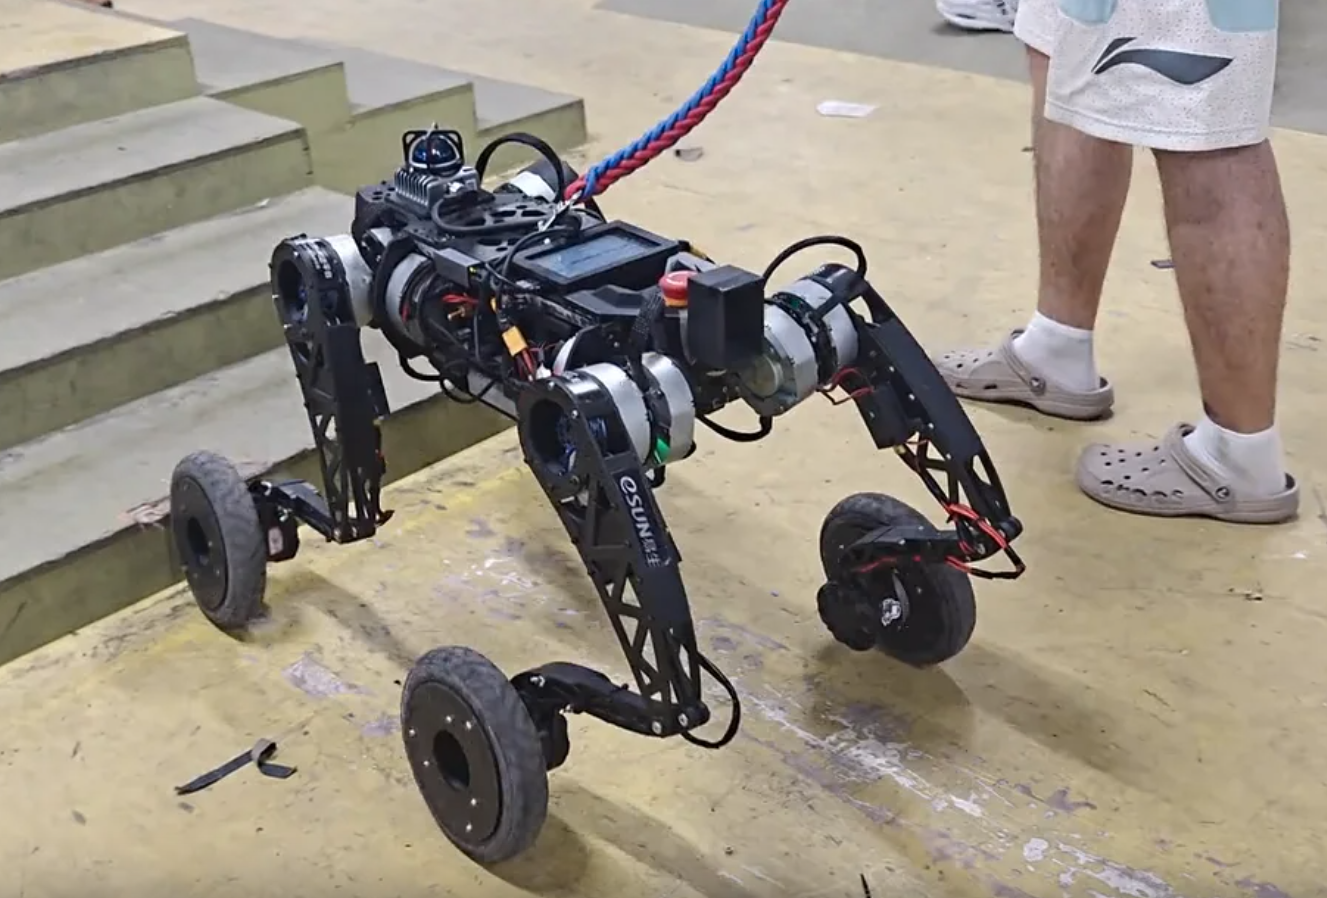
\includegraphics[width=0.64\linewidth,alt={轮式四足机器人示例。}]{figures/轮式四足机器人示例.png}
\caption{轮式四足机器人示例}
\label{fig:quadruped-field-debug}
\end{figure}

\subsection{问题要求}

\textbf{问题一：}根据多个检测点坐标及同一干扰源的示向度，给出采用交会定位法计算多边形定位区域直径的算法，并判断以该直径为直径的圆是否能够覆盖定位区域。

\textbf{问题二：}对于已在一个检测点测得示向度的全向干扰源，确定第二个检测点的选择策略及候选区域，以获得较好的定位效果。

\textbf{问题三：}目标区域内有 $10$ 至 $16$ 个全向干扰源，具体数量未知。机器狗从原点出发，测向机初始频道为 $1$，需制定自动搜索、定位与清除策略，使其在清除全部干扰源的前提下尽量减少总耗时。

\textbf{问题四：}在总数范围和初始条件不变的情况下，考虑全向与定向干扰源混合分布，且定向干扰源的数量及方向未知；定向源仅在发射方向两侧各 $90^\circ$ 内辐射信号，需据此制定检测与清除策略。

对问题三、四，均需通过演练检验清除比例和平均定位清除时间。清除比例为清除数与总数之比，平均定位清除时间为任务总耗时与清除数之比；并按题目要求分别报告三次正式测试结果及提供对应日志。

\clearpage
%
\section{问题分析}\label{sec:problem-analysis}

本题的核心是在观测不完备的条件下，协调定位精度、搜索完整性与任务耗时。示向度误差使单次检测只能确定源所在的角域，有限接收范围又限制了后续检测位置；在多源情形下，机器狗还须兼顾未知源的发现与已知源的清除。因此，本文依次分析定位区域的几何性质、单源主动选点及多源任务调度，并以实际反馈维持各阶段之间的信息一致性。

\subsection{问题一的分析}

问题一首先需要把测向误差转化为源位置约束。每次示向度对应一个由两条边界射线限定的角域，多次观测的交集构成定位区域。由于不同测点的几何关系可能使交集为空或无界，计算直径前应先检验区域的可行性与有界性；在非空有界情形下，可利用凸多边形的顶点求最远点对，避免遍历区域内的连续点集。

直径计算与覆盖检验需要分别处理。最远点对距离只约束点与点之间的间隔，不能直接保证所有候选位置均落在以该线段为直径的圆内。因此，应另行检验各顶点到圆心的距离，并构造反例说明两者的区别。这一区分也为后续清除提供依据：可靠清除应建立在覆盖整个可行区域的距离保证上，不能仅凭区域直径判断。

\subsection{问题二的分析}

问题二的难点在于第二次观测尚未发生，真实源的位置和接收半径均未知。直接沿首测方向接近可能保留较长的定位区域，过大的横向移动又可能导致失去信号。为此，先将目标区域、首测角域与接收半径上界相交，形成包含真实源的候选区域，再利用接收半径下界筛选能够对全部候选源位置保证接收的检测点。

在该可行范围内，依据定位区域的长轴构造具有不同交会角度的有限探点，通过名义观测估计区域收缩，并同时计入移动代价。名义源点只用于比较动作，不替代实际观测；执行检测后，仍须根据真实反馈更新定位区域，并检查是否达到可靠清除尺度。由此将选点的可行性保证与选点效率的实验评价分开。

\subsection{问题三的分析}

问题三同时包含未知源的发现、已知源的定位清除以及任务完成判定。仅清除当前已经发现的源不能保证全清，而逐站重复扫描全部频道又会增加行程与检测费用。因此，先以接收半径下界构造全域发现覆盖，再将剩余覆盖站与已知源组成两类任务，在保证不遗漏源的前提下联合安排访问顺序。

由于新观测会改变定位区域和任务集合，采用滚动规划：每轮暂时冻结任务代表位置及代理费用，以状态压缩和有预算的 A* 搜索比较任务顺序，仅执行首项任务后重新规划。源处理过程中调用第二问的主动定位模块，并利用共享测量与有严格依据的静默推断减少重复检测；定位不足时以有限光学网格完成局部搜索。最后分别检验全清比例、动作计费用时及程序计算开销，通过同场景对照和消融分析判断各策略的实际作用。

\subsection{问题四的分析}

定向源只向发射方向两侧各 $90^\circ$ 的半平面辐射，无信号既可能因为距离超限，也可能因为检测点在发射范围之外。这使第三问的三处做法不再成立：无信号点不能再用来推距离；覆盖站只按距离布置，不能保证发现背对着检测点的源；贴着边界朝外发射的源，在场内任何位置都收不到。因此，问题四需要先把发现条件改成对任意发射方向都成立的几何条件，并允许检测点放到场地外侧；再为无信号反馈找到在两类源上都成立的用法，例如成对布置检测点，以及把确定在接收范围内的无信号点和有信号点联合起来限制方向和位置。任务安排沿用滚动规划的框架，但每一步的候选动作更多，多测一次是否划算不容易靠规则判断，可以用离线模拟的数据训练一个评分来辅助决策，同时用几何条件守住不漏源、不误清的底线。

%
\section{模型假设}\label{sec:model-assumptions}

在题设设备参数与动作规则的基础上，明确本文模型采用的以下工作条件。其中，全向接收与静默推断的条件仅用于第二、三问；第四问的附加条件见第 7、8 条。

\begin{enumerate}
  \item \textbf{平面运动与坐标准确性。}按题设忽略设备与干扰源的高度差，将两者表示为平面点。假定机器狗能够准确获得自身位置并到达指定坐标，两点间按直线匀速移动，不另计位置误差、地形绕行、加减速与转向代价，使移动耗时可由欧氏距离计算。

  \item \textbf{源参数稳定且各源互不影响。}假定干扰源在一次任务中保持静止，未清除前其频道、发射功率及有效接收半径不变。各源信号按题设互不影响，清除一个源不改变其他源的接收条件。源位置、具体数量及接收半径的真实值均不作为决策输入，只利用公开范围与真实反馈逐步约束。

  \item \textbf{全向信号遵循距离门限。}对于第二、三问中的未清除全向源，是否接收到信号仅由检测距离与该源固定接收半径决定，不额外引入遮挡、间歇发射或随机漏检。距离不超过 $5\,\mathrm{m}$ 时按题设返回近场反馈而非示向度；该条件支持保证接收域、发现覆盖及历史静默推断的建立。

  \item \textbf{测角误差按有界不确定性处理。}保留题设 $\pm1^\circ$ 的误差界，不假定不同地点的误差相互独立或服从特定概率分布，也不通过同地点重复检测缩小误差界。实现中对保留两位小数的示向度采用 $1.005^\circ$ 计算半角，仅用于容纳舍入余量，区域更新仍以真实反馈为依据。

  \item \textbf{动作顺序执行并按规则计费。}移动、换频、检测、光学定位与清除按动作顺序执行，任务总耗时为实际动作费用之和。光学尝试失败时仍计定位耗时，成功后再计清除耗时；算法计算时间另行记录，不与机器狗的动作计费用时混合。

  \item \textbf{光学操作遵循题设距离条件。}假定设备正常工作，在距目标源不超过 $20\,\mathrm{m}$ 时能够完成光学精确定位和清除，其成功条件不依赖信号辐射方向。算法仅在收到真实成功反馈后登记清除；有限步全清的保证以时间和动作预算足够为前提，超时或未确认的请求不作为成功。

  \item \textbf{定向源的辐射范围为半平面。}第四问中的定向源只向发射方向两侧各 $90^\circ$ 的范围辐射，即只有位于过源位置、垂直于发射方向的直线所限定的闭半平面内，且距离不超过接收半径的位置才能收到信号；发射方向在一次任务中固定，两类源的数量和比例均未知。近场反馈同样受该范围限制，光学定位和清除只取决于距离。

  \item \textbf{机器狗可在目标区域外侧附近停留检测。}题目只规定干扰源位于半径 $1800$ m 的目标区域内，未限制机器狗的活动范围；第四问的检测站中有一环位于半径 $1865$ m 的圆周上，用于发现贴着边界朝外发射的定向源。
\end{enumerate}

%
\clearpage
% 各问正文沿用自己的数学记号；此表汇总含义，方便手动修改时对照。
\section{符号说明}


第一问用检测点 $S_i$、候选源位置 $X$ 和定位域 $P$ 描述交会几何；
第二、三问分别用 $x_t$、$p$ 和 $\widehat C_f$ 表示检测位置、源位置及其凸外包区域；
第四问增加发射方向 $u$ 和正、负观测位置 $x^+$、$x^-$。
表\ref{tab:symbols}汇总主要记号，各问的局部参数在使用处定义。

\begin{center}
\small
\captionof{table}{主要符号与含义}\label{tab:symbols}
\begin{tabularx}{\linewidth}{@{}>{\raggedright\arraybackslash}p{0.22\linewidth}X@{}}
\toprule
符号 & 含义 \\
\midrule
$\Omega$ & 半径为1800 m的目标圆域 \\
$S_i=(x_i,y_i)$ & 第一问中第 $i$ 个检测点的位置 \\
$X,\ P$ & 第一问中的候选源位置与定位区域 \\
$v_1,\ldots,v_h$ & 定位区域的顶点 \\
$D,\ C_0$ & 定位区域的直径与最远顶点对的中点 \\
$\theta_i,\ \varepsilon$ & 示向度与题面测角误差界，$\varepsilon=1^\circ$ \\
$\varphi_i,\ \delta$ & 第一问采用的弧度角，$\varphi_i=\pi\theta_i/180$、$\delta=\pi\varepsilon/180$ \\
$\bar\varepsilon$ & 第二、三问包含舍入余量的计算误差界，取 $1.005^\circ$ \\
$f,\ p,\ x_t$ & 测向频道、源位置与当前机器人位置 \\
$R_f$ & 固定但未知的接收半径，$1000\le R_f\le1500$ m \\
$\widehat C_f,\ Q_f$ & 源位置凸外包区域与保证再次接收的测点域 \\
$z(C),\ \rho(C)$ & 区域 $C$ 的最小包围圆圆心与半径 \\
$v,\ L,\ T$ & 移动速度（5 m/s）、实际路长与动作计费用时 \\
$\mathcal D_t,\ \mathcal K_t$ & 已发现和已清除的频道集合 \\
$M,\ j$ & 已完成任务集合（位掩码存储）与最后一个任务 \\
$U_t,\ L_t$ & 当前冻结规划问题的上界与下界 \\
$u$ & 第四问中定向源的发射方向，单位向量 \\
$x^+,\ x^-$ & 某频道收到信号与未收到信号的检测位置 \\
$R_{\min}$ & 由有信号点推出的接收半径下界 \\
$q^{\pm},\ t,\ h$ & 成对检测点及其沿示向方向的前进距离与横向偏移 \\
\bottomrule
\end{tabularx}
\end{center}

第二问的主动检测点选择构成第三问多源搜索的局部定位模块。
实验中的耗时采用题目动作计费口径，程序计算时间另行报告。


%
\section{模型的建立与求解}\label{sec:models}


% ===== 问题一正文 =====
% 在本子文件修改问题一正文，公式和图表编号由主文件统一管理。
\subsection{问题一：交会定位法计算多边形定位区域直径}\label{sec:q1}
\subsubsection{计算干扰源定位区域}\label{sec:q1-1}

设机器狗在 $n$ 个位置 $S_i=(x_i,y_i)$ 处对该干扰源测得示向度 $\theta_i$。$\theta_i$ 是自正东逆时针量到“检测点指向干扰源”方向的角度，但它并不是干扰源的真实方位：真实方位落在 $\theta_i$ 两侧各 $1^\circ$ 内。因此，干扰源一定位于以 $S_i$ 为顶点、方向在 $\theta_i\pm1^\circ$ 之间的一个 $2^\circ$ 窄楔形内。

现在要把“点在楔形内”写成数学不等式。记 $\varphi_i=\pi\theta_i/180$，$\delta=\pi\varepsilon/180=\pi/180$，楔形的两条边方向分别为

\[
u_i^-=\begin{pmatrix}\cos(\varphi_i-\delta)\\ \sin(\varphi_i-\delta)\end{pmatrix},\qquad
u_i^+=\begin{pmatrix}\cos(\varphi_i+\delta)\\ \sin(\varphi_i+\delta)\end{pmatrix},
\]

其中 $u_i^-$ 对应偏转角度的下限 $\varphi_i-\delta$，$u_i^+$ 对应上限 $\varphi_i+\delta$。判断一个点在两条边的哪一侧，可以用二维向量的叉积：对 $a=(a_x,a_y)$、$b=(b_x,b_y)$，定义 $a\times b=a_xb_y-a_yb_x$，它大于零说明 $b$ 在 $a$ 的逆时针一侧，小于零说明在顺时针一侧。于是，点 $X=(x,y)$ 落在楔形内的条件是

\begin{equation}\label{eq:q1-1}
u_i^-\times(X-S_i)\ge 0,\qquad u_i^+\times(X-S_i)\le 0.
\end{equation}

第一式要求 $X-S_i$ 不越过下边 $u_i^-$（在其逆时针一侧），第二式要求不越过上边 $u_i^+$（在其顺时针一侧），两式合起来就是把 $X$ 夹在两条边之间。

将式\eqref{eq:q1-1} 展开：

\begin{equation}\label{eq:q1-2}
\begin{aligned}
\sin(\varphi_i-\delta)(x-x_i)-\cos(\varphi_i-\delta)(y-y_i)&\le 0,\\
-\sin(\varphi_i+\delta)(x-x_i)+\cos(\varphi_i+\delta)(y-y_i)&\le 0.
\end{aligned}
\end{equation}

这两个式子都是 $x$、$y$ 的一次不等式，形如 $ax+by\le c$。满足 $ax+by\le c$ 的点集是直线 $ax+by=c$ 一侧的半个平面，称为半平面，它是一个凸集。式\eqref{eq:q1-2} 的两个不等式分别对应楔形的两条边，它们的交集就是该楔形。这样就把几何上“点在楔形内”的条件，转化成了代数上两个线性不等式同时成立。

$n$ 次测向后，干扰源必须同时落在每个楔形内，也就是要同时满足全部 $2n$ 个不等式。将它们统一写成 $a_jx+b_jy\le c_j$，得到定位区域

\begin{equation}\label{eq:q1-3}
P=\bigcap_{j=1}^{2n}\left\{(x,y):a_jx+b_jy\le c_j\right\}.
\end{equation}

$P$ 是 $2n$ 个半平面的交。半平面是凸集，凸集之交仍是凸集，故 $P$ 为凸集；在非空且有界时，$P$ 是\textbf{凸多边形}，退化情形为线段或点。题目图 2 中的红色四边形就是 $n=2$ 时两个楔形求交的结果。每增加一次有效测向，约束增加两条，定位区域随之收缩。

\subsubsection{求定位区域的直径}\label{sec:q1-2}

定位区域 $P$ 是凸多边形，现在要求它的直径---区域内距离最远的一对点之间的距离。

\textbf{首先确认区域有界。} 并非任意一组测向都能定出有限的区域。若各检测点近似共线、示向度方向接近平行，楔形之交沿某方向无限延伸，区域无界，直径为无穷大；若某次读数偏差较大，各楔形可能互不相容，区域为空。这两种情形都需要先排除。

具体做法是用线性规划：先检验约束组 $\{a_jx+b_jy\le c_j\}$ 是否可行，不可行说明数据矛盾，应剔除异常的测向数据；若可行，再分别求 $x$、$-x$、$y$、$-y$ 在约束下的最大值，四者均有限当且仅当 $P$ 有界。注意，无界区域也可能有若干有限顶点（例如楔形的尖端），若跳过这一步直接取顶点对距离，会把本应为无穷的直径误报成有限值。

\textbf{确认有界后，求出全部顶点。} 凸多边形的每个顶点都是某两条边界直线的交点。对直线 $a_jx+b_jy=c_j$ 与 $a_kx+b_ky=c_k$，记 $\Delta_{jk}=a_jb_k-a_kb_j$，当 $\Delta_{jk}\ne0$ 时交点为

\begin{equation}\label{eq:q1-4}
x_{jk}=\frac{c_jb_k-b_jc_k}{\Delta_{jk}},\qquad
y_{jk}=\frac{a_jc_k-c_ja_k}{\Delta_{jk}}.
\end{equation}

$\Delta_{jk}=0$ 时两直线平行，没有孤立交点，跳过。求出的交点未必在区域内，需代回全部 $2n$ 个约束检验，保留满足所有不等式者；去重后即得顶点集 $\{v_1,\dots,v_h\}$。

\textbf{有了顶点，直径就可以确定。} 按题目定义，$D=\max_{X,Y\in P}\|X-Y\|_2$。因为 $P$ 是凸多边形，我们证明这个最大值一定在顶点对上取得：

\begin{equation}\label{eq:q1-5}
D=\max_{1\le i<j\le h}\|v_i-v_j\|_2 .
\end{equation}

理由如下。凸多边形是其全部顶点的凸包，因此 $P$ 中任意一点都可写为顶点的凸组合：存在 $\lambda_i\ge0$、$\sum_i\lambda_i=1$，使 $X=\sum_i\lambda_iv_i$；同理 $Y=\sum_j\mu_jv_j$，$\mu_j\ge0$、$\sum_j\mu_j=1$。两式相减得

\[
X-Y=\sum_{i,j}\lambda_i\mu_j(v_i-v_j),
\qquad
\sum_{i,j}\lambda_i\mu_j=\left(\sum_i\lambda_i\right)\left(\sum_j\mu_j\right)=1 .
\]

由三角不等式，

\[
\|X-Y\|\le\sum_{i,j}\lambda_i\mu_j\|v_i-v_j\|\le\max_{i,j}\|v_i-v_j\|\cdot1=\max_{i,j}\|v_i-v_j\|,
\]

即区域内任意两点的距离都不超过最远顶点对的距离。而最远顶点对本身就是区域内的点，所以这个上界可以取到。式\eqref{eq:q1-5} 成立。

综上，求直径的完整流程为：

\par\medskip
\noindent\begin{minipage}{\linewidth}
\small
\refstepcounter{algorithm}\label{alg:q1-diameter}
\textbf{算法\thealgorithm：定位区域直径计算}\par\smallskip
\noindent\textbf{输入：}检测点 $S_i$、示向度 $\theta_i$，$i=1,\dots,n$
\begin{enumerate}
\setlength{\itemsep}{2pt}
\setlength{\parskip}{0pt}
\item 按式\eqref{eq:q1-2} 将每次测向写成两个半平面约束；
\item 线性规划检验可行性与有界性；
\item 按式\eqref{eq:q1-4} 求每对边界直线的交点；
\item 保留满足全部约束的交点并去重，得顶点集；
\item 比较所有顶点对的距离，取最大者 $(A,B)$，$D=|AB|$。
\end{enumerate}
\end{minipage}
\par\medskip

边界直线共 $2n$ 条，交点约 $\binom{2n}{2}=O(n^2)$ 个，每个交点检验约束需 $O(n)$，顶点数不超过 $2n$，比较顶点对为 $O(n^2)$，总计算量 $O(n^3)$。本题 $n$ 一般不超过十几，计算量完全可以实时完成。

\subsubsection{判断直径圆能否覆盖定位区域}\label{sec:q1-3}

机器狗的光学探测仪只能在距干扰源 $20$ m 以内工作。如果以定位区域直径 $D$ 为直径画一个圆，能盖住整个区域，那么只要 $D\le40$ m，机器狗走到圆心就能保证清除成功---这比计算最小包围圆要简单得多。所以问题是：这样的圆真的能盖住整个区域吗？

首先要确定圆心。设最远的一对顶点为 $A$、$B$，距离为 $D$。若半径 $D/2$、圆心 $C$ 的圆覆盖了 $P$，则 $A$、$B$ 都在圆内，即 $\|A-C\|\le D/2$、$\|C-B\|\le D/2$。代入三角不等式

\[
D=\|A-B\|\le\|A-C\|+\|C-B\|\le\frac D2+\frac D2=D .
\]

不等式的两端相等，故中间每一步都取等号：$\|A-C\|=\|C-B\|=D/2$，且 $C$ 在线段 $AB$ 上。这两个条件合起来，$C$ 只能是 $AB$ 的中点 $C_0=(A+B)/2$。圆是凸集，覆盖全部顶点就覆盖了整个凸多边形，所以判据为

\begin{equation}\label{eq:q1-6}
\max_{1\le i\le h}\|v_i-C_0\|\le\frac D2 .
\end{equation}

式\eqref{eq:q1-6} 是否一定满足？下面说明它可以不成立，并给出一个满足题设条件的具体反例。

\textbf{构造思路：} 要让直径圆盖不住区域，需要找到这样一个顶点：它已经跑到了直径圆外面，但它到其他顶点的距离还没有超过原来的直径---直径没变，圆却已经不够大了。

先用归一化的坐标把这个想法量化。取 $A=(-1,0)$、$B=(1,0)$，$|AB|=2$，直径圆以原点为圆心、半径为 $1$。在上方放一个点 $U=(0,h)$，希望它同时满足：

\begin{itemize}
\item 跑到圆外：$h>1$；
\item 不改变直径：$|UA|=|UB|=\sqrt{1+h^2}\le2$，即 $h\le\sqrt{3}$。
\end{itemize}

两个条件合起来是 $1<h\le\sqrt{3}$，这个区间非空。直观地理解：上顶点刚越过圆的最高点时，它离左右两端还不够远，不会产生更长的边。

取 $h=1.5$，则 $|UA|=\sqrt{3.25}\approx1.803<2$，直径仍为 $2$；而上顶点距圆心 $1.5$，超出半径 $50\%$。反例的形状就有了：底边为 $2$、高为 $1.5$ 的等腰三角形。

\textbf{用测向数据实现该形状：} 将坐标放大到米，目标三角形的三个顶点为

\[
A=(-10,\,0),\quad B=(10,\,0),\quad U=(0,\,15).
\]

三条边分别是 $y=0$（底边）、$y=1.5x+15$（左腰）、$y=-1.5x+15$（右腰）。三角形有 $3$ 条边，而每个检测点的楔形提供 $2$ 条边界线，因此用 $3$ 个检测点（$6$ 条边界线）即可实现：让其中 $3$ 条边界线分别与三角形的三条边重合，另外 $3$ 条不切入三角形内部。具体取法见表\ref{tab:q1-counterexample}。

\begin{center}
\begin{minipage}{\linewidth}
\centering
\captionof{table}{反例的检测数据（误差界 $\pm1^\circ$）}\label{tab:q1-counterexample}

\renewcommand{\arraystretch}{1.3}
\begin{tabularx}{0.98\linewidth}{>{\centering\arraybackslash}p{0.22\linewidth}>{\centering\arraybackslash}p{0.20\linewidth}>{\raggedright\arraybackslash}X}
\toprule
\textbf{检测点 $S_i$（m）} & \textbf{示向度 $\theta_i$} & \textbf{起决定作用的边界} \\
\midrule
$(-500,\,0)$ & $1^\circ$ & 下边界方向为 $0^\circ$，给出 $y\ge0$（底边） \\
$(-310,\,-450)$ & $\approx55.31^\circ$ & 上边界方向为 $\arctan(1.5)$，给出 $y\le1.5x+15$（左腰） \\
$(310,\,-450)$ & $\approx124.69^\circ$ & 下边界方向为 $180^\circ-\arctan(1.5)$，给出 $y\le-1.5x+15$（右腰） \\
\bottomrule
\end{tabularx}
\end{minipage}
\end{center}

其中第二个检测点的示向度取 $\theta_2=\arctan(1.5)-1^\circ\approx55.31^\circ$，第三个取 $\theta_3=181^\circ-\arctan(1.5)\approx124.69^\circ$。将三角形的三个顶点分别代入每个楔形的另一条边界线，可以验证它们均满足约束（不被裁掉），因此 $6$ 个半平面的交恰好就是三角形 $ABU$。

现在检验覆盖性。边长为 $|AB|=20$，$|AU|=|BU|=\sqrt{325}\approx18.03$，直径 $D=20$ m 由 $A$、$B$ 取得。直径圆圆心 $C_0=(0,\,0)$，半径 $D/2=10$ m。而上顶点到圆心的距离为

\[
\|U-C_0\|=15\ \text{m}>10\ \text{m}=\frac D2,
\]

超出半径 $5$ m，式\eqref{eq:q1-6} 不成立。

\begin{center}
\begin{minipage}{\linewidth}
\centering
\QOneCaseFigure
\captionof{figure}{三次测向的角域交集与直径圆覆盖检验。左图按实际比例绘制三个误差角域；右图放大定位三角形，红色圆的半径为 $10$ m，上顶点超出 $5$ m。}
\label{fig:q1-counterexample}
\end{minipage}
\end{center}

三个检测点到三角形中心的距离均约 $500$ m，在有效接收半径内；三角形整体位于半径 $1800$ m 的目标区域内，是完全合理的探测场景。于是问题一的第二问答案为否：

\textbf{以定位区域直径为直径的圆，不一定能覆盖该定位区域。}


%
% ===== 问题二正文 =====
% 问题二正文；三张示意图的 TikZ 宏在 figures/q2_schematics.tex 中定义。
\subsection{问题二：第二检测点选择模型的建立与求解}\label{sec:q2}

问题二中只进行了一次测向，需要确定第二个检测点的位置。此时干扰源的位置和接收半径均未知，第二检测点的优劣只能依据首测信息判断。本节先在模型准备中给出首测后源的可能范围，并分析第二次测向的几何作用；再以第二检测点为决策变量建立优化模型；然后给出模型的求解方法；最后用实际观测数据检验。本节建立的单源定位模型在第三问中反复调用。

\subsubsection{模型准备}\label{sec:q2-1}

\textbf{（1）符号约定。}记所考察的频道为 $f$，源的位置为 $p$，首个检测点为 $x_1$，测得的示向度为 $\theta_1$，示向方向的单位向量记为 $u(\theta_1)=(\cos\theta_1,\sin\theta_1)$。场地为半径 $1800$ m 的圆，记作 $\Omega$；$B(x,r)$ 表示以 $x$ 为圆心、半径为 $r$ 的圆盘。接收半径 $R_f$ 在一次任务中固定，仅知其取值范围为 $1000$ 至 $1500$ m。测角误差按题设取 $\pm\varepsilon$，$\varepsilon=1^\circ$。

\textbf{（2）首测后的定位区域。}首测得到示向度 $\theta_1$ 后，源的位置 $p$ 需同时满足三个条件：

\begin{itemize}
\item \textbf{角度条件：}$p$ 位于示向度 $\theta_1\pm1^\circ$ 所夹的楔形 $W(x_1,\theta_1)$ 内，不等式写法同第一问的式\eqref{eq:q1-1}；
\item \textbf{距离条件：}在 $x_1$ 收到了信号，故 $\|p-x_1\|\le1500$ m；
\item \textbf{场地条件：}$p\in\Omega$。
\end{itemize}

三者的交集即首测后源可能所在的范围，沿用第一问的叫法称为定位区域：

\begin{equation}\label{eq:q2-1}
C_f^{(1)}=\Omega\cap B(x_1,1500)\cap W(x_1,\theta_1).
\end{equation}

\textbf{（3）定位区域的多边形近似。}$C_f^{(1)}$ 的边界含有两段圆弧，不便像第一问那样用顶点计算。将两个圆分别换成其外切正 $128$ 边形，得到凸多边形 $\widehat C_f^{(1)}\supseteq C_f^{(1)}$。采用外切而非内接多边形，是为了使近似只扩大、不缩小区域，真实源不会因近似而被排除。后文的选点和清除判断均以 $\widehat C_f^{(1)}$ 为准。另记 $\rho(C)$、$z(C)$ 分别为区域 $C$ 的最小外接圆半径和圆心，第三问中将该圆简称为包围圆。

\textbf{（4）第二次测向的几何作用。}首测后的定位区域是一条张角 $2^\circ$、长达 $1500$ m 的窄带：角度已经足够准，缺的是距离。第二次测向要做的，是用第二条视线把这条窄带截断，截断的效果取决于两条视线的夹角，即测量学中的交会角。图\ref{fig:q2-cross}比较了两种方案：

\begin{itemize}
\item \textbf{沿示向方向前进再测：}两条视线几乎平行，只截去窄带靠近 $x_1$ 的一段，剩余部分仍然狭长；
\item \textbf{横向偏移后再测：}两条视线斜交，交集只是一个小四边形。
\end{itemize}

\begin{center}
\begin{minipage}{\linewidth}
\centering
\QTwoCrossFigure
\captionof{figure}{两种第二检测点的比较。沿示向方向前进只能截短楔形；横向偏移后两条视线斜交，定位区域才明显缩小。}
\label{fig:q2-cross}
\end{minipage}
\end{center}

两种方案的差别可以用交会角定量刻画。设两次检测点到源的距离分别为 $d_1$、$d_2$，交会角为 $\gamma$。每个楔形在源附近的宽度约为 $2d_i\varepsilon$（$\varepsilon$ 按弧度计），两条窄带斜交所得四边形的对角线长度约为

\begin{equation}\label{eq:q2-2}
D\approx\frac{2(d_1+d_2)\,\varepsilon}{\sin\gamma}.
\end{equation}

由式\eqref{eq:q2-2}，$\gamma$ 越接近 $90^\circ$，定位区域越小；$d_2$ 越小，定位区域也越小。因此第二检测点应当靠近源，并与首测视线拉开一定的横向距离。

\textbf{（5）接收范围的限制。}横向偏移不能没有限度。示向度只有在源的接收半径之内才能测得，而接收半径未知，只知道不小于 $1000$ m。第二检测点若离源过远，将收不到信号，移动和检测的时间随之浪费。因此第二检测点的选择需要兼顾两方面：增大交会角以缩小定位区域，保证接收以免测向失败。前者构成下面模型的目标函数，后者构成约束条件。

\subsubsection{模型的建立}\label{sec:q2-2}

\textbf{（1）决策变量。}待确定的是第二检测点的位置，记为 $x\in\mathbb R^2$。为使模型在第三问中同样适用，记机器狗当前所在位置为 $x_0$：第二问中 $x_0=x_1$，第三问中为当时的实时位置；当前的定位区域记为 $\widehat C_f$，第二问中即 $\widehat C_f^{(1)}$。

\textbf{（2）约束条件。}第一条约束是保证接收。第二次测向若收不到信号，便无法形成双站交会。接收半径虽然未知，但不小于 $1000$ m；因此只要 $x$ 到源的每一个可能位置的距离都不超过 $1000$ m，则无论源的实际位置和接收半径如何，到达 $x$ 后必定能收到信号。满足该条件的位置集合称为可靠接收区，记作 $Q_f$。该条件涉及区域内的无穷多个点，但由于区域是凸多边形，只需检验其顶点：

\begin{equation}\label{eq:q2-3}
Q_f=\bigl\{x:\ \|x-a\|\le1000\ \text{对}\ \widehat C_f\ \text{的每个顶点}\ a\ \text{成立}\bigr\}.
\end{equation}

理由与第一问求直径时相同：多边形内任一点都是顶点的凸组合，它到 $x$ 的距离不超过各顶点到 $x$ 距离的最大值；而顶点本身属于区域。因此到所有顶点的距离不超过 $1000$ m，等价于到区域内所有点的距离不超过 $1000$ m，检验一个候选点只需计算与顶点个数相同的若干次距离。$Q_f$ 是有限个圆盘的交集，因而是凸集。

式\eqref{eq:q2-3}便于计算，但没有直接给出该区域的位置和大小，下面给出它的一个可以直接写出的子区域。记 $\widetilde R$ 为 $\widehat C_f^{(1)}$ 的顶点到 $x_1$ 的最大距离（略大于 $1500$ m），则整个定位区域落在以 $x_1$ 为顶点、半径 $\widetilde R$、半角 $\varepsilon$ 的扇形内。过 $x_1$ 和扇形的两个远端点作圆，其圆心 $z_0$ 位于示向线上，半径为

\begin{equation}\label{eq:q2-4}
r_0=\frac{\widetilde R}{2\cos\varepsilon}\approx750\ \text{m},\qquad z_0=x_1+r_0\,u(\theta_1).
\end{equation}

该圆恰好覆盖整个扇形：扇形内任一点到 $z_0$ 的距离平方是它到 $x_1$ 距离的凸函数，最大值只能在扇形顶点或远端弧上取得，而这两处到 $z_0$ 的距离均不超过 $r_0$。于是，以 $z_0$ 为圆心、半径 $1000-r_0\approx250$ m 的圆盘内任一点 $x$，到任一可能源 $p$ 的距离满足 $\|x-p\|\le\|x-z_0\|+\|z_0-p\|\le1000$，即该圆盘整体包含于 $Q_f$。换言之，沿示向方向前进约 $750$ m，以该处为圆心、半径约 $250$ m 的圆盘内的任一位置，都能保证再次收到信号。场地边界只会缩小定位区域、扩大 $Q_f$，因此上述结论对任意首测位置均成立。图\ref{fig:q23-1}按实际比例画出了首测楔形、覆盖圆和可靠接收区。

\begin{center}
\begin{minipage}{\linewidth}
\centering
\QTwoRegionFigure
\captionof{figure}{首测楔形、覆盖圆与可靠接收区（按实际比例绘制）。蓝色为可靠接收区 $Q_f$ 的一部分，由包含楔形的三角形的三个顶点按式\eqref{eq:q2-3}画出；虚线圆为覆盖整个楔形的圆 $B(z_0,r_0)$；绿色为以 $z_0$ 为圆心、半径约 $250$ m 的圆盘，整体落在 $Q_f$ 内。}
\label{fig:q23-1}
\end{minipage}
\end{center}

式\eqref{eq:q2-3}只是保证接收的充分条件，并非能够接收的最大范围。首测收到信号还蕴含 $R_f\ge\|p-x_1\|$，若将这一信息一并利用，可以进一步放宽部分位置。本文统一采用 $1000$ m 这一界限，一方面计算简单，另一方面在第三问的多次测向中可以直接沿用。

第二条约束是不重复检测：$x$ 不能取该频道已经测过的位置。题设指出同一地点重复检测不能消除误差，重复检测只会增加耗时。

\textbf{（3）目标函数。}选点的目的是减少任务耗时，因此以前往某点测向一次所引起的各项时间之和作为代价。测向后定位区域收缩的程度取决于源的真实位置，而后者未知。本文的处理办法是假设源位于定位区域内的若干代表位置上：区域中心 $z=z(\widehat C_f)$，以及从顶点中均匀选取的至多 $4$ 个点，各自向中心移动四分之一（选取靠近顶点的位置是为了兼顾源处于区域边缘的情形，向内移动则避免代表位置恰好落在边界上），记为 $p^{(1)},\dots,p^{(h)}$，$h\le5$。对候选点 $x$ 和假想的源位置 $p^{(k)}$，由 $x$ 指向 $p^{(k)}$ 的方向即为一条不含误差的示向度，将其作为新的测向结果，用第一问的方法在区域上增加一个楔形约束，求出新区域的包围圆半径，记为 $r_k(x)$。若 $x$ 与 $p^{(k)}$ 的距离不超过 $5$ m，按题设设备将给出近场反馈，可直接在该处清除。

移动速度 $v=5$ m/s，可靠清除的半径门限取 $r_c=19.9$ m（略小于 $20$ m 的光学清除距离）。候选点 $x$ 的代价定义为

\begin{equation}\label{eq:q2-5}
J(x)=\frac{\|x-x_0\|}{v}
+\frac1h\sum_{k=1}^{h}\left[\frac{\|x-p^{(k)}\|}{v}+P_k(x)\right].
\end{equation}

三项依次为：由当前位置移动到候选点的时间；测向后由候选点移动到源的时间，对 $h$ 个假想位置取平均；测向后仍未达到清除条件的罚时 $P_k(x)$。罚时的取法为：若 $r_k(x)$ 不超过 $r_c$，或已得到近场反馈，则罚时为零；否则至少还需一次检测和一次换频，计 $6$ s，半径每超出门限 $1$ m 再加 $0.1$ s，以反映后续额外的移动。换频与本次检测的时间对所有候选点相同，不影响排序，故不计入。

\textbf{（4）模型汇总。}综上，第二检测点的选择模型为

\begin{equation}\label{eq:q2-6}
\begin{aligned}
\min_{x}\quad & J(x)\\
\text{s.t.}\quad & \|x-a\|\le1000,\quad a\ \text{为}\ \widehat C_f\ \text{的每个顶点},\\
& x\ \text{不是该频道已测过的位置}.
\end{aligned}
\end{equation}

约束条件保证第二次测向必定收到信号，目标函数在移动路程与测后剩余区域之间取得平衡。等权的假想位置仅用于比较候选点，并不代表源位置的概率分布，因此模型\eqref{eq:q2-6}给出的是一条可执行的选点规则，而非所有情形下的最优解。实际到达第二检测点并完成测向后，只用真实示向度更新定位区域，假想位置不再参与。

\subsubsection{模型的求解}\label{sec:q2-3}

模型\eqref{eq:q2-6}的可行域 $Q_f$ 是连续区域，目标函数中又含有区域求交和最小外接圆的计算，难以求得解析解。考虑到实际只需要一个足够好的检测点，本文采用有限候选点枚举的方法求解：在可行域内布设若干具有代表性的候选点，逐一计算代价，取代价最小者。

\textbf{（1）候选点的生成。}候选点分两组，布设方式见图\ref{fig:q2-cand}。

第一组沿前进方向布设。在 $x_0$ 到区域中心 $z$ 的连线上取中点和终点，各自向两侧横向偏移 $50$ m 和 $150$ m，连同中心 $z$ 共 $9$ 个点。这一组保证候选中总有靠近区域、路程较短的位置。

第二组沿定位区域的长轴布设。由式\eqref{eq:q2-2}，最需要截断的是区域最长的方向。取多边形中相距最远的一对顶点，其连线方向为长轴；将全部顶点投影到长轴上，得到区域沿长轴的长度 $w$。在长轴的 $1/4$、$3/8$、$5/8$、$3/4$ 四个分位点上，各取轴上一点及两侧横向偏移 $b_*$ 的两点，再在中心 $z$ 两侧各取一个横向偏移 $b_*$ 的点，共 $14$ 个点。横向偏移量随区域大小调整：

\begin{equation}\label{eq:q2-7}
b_*=\min\{200,\ \max\{20,\ w/8\}\}\ \text{m},
\end{equation}

即取区域长度的八分之一，并限制在 $20$ m 至 $200$ m 之间。区域越长横向偏移越大，上限 $200$ m 用于避免候选点超出可靠接收区。分位点中加入靠内的 $3/8$ 和 $5/8$，是因为首测楔形很长时，$1/4$ 和 $3/4$ 处的横向偏移点往往已超出可靠接收区，靠内的分位点可以保留横向选择。

两组候选点合并后，去除重复点、该频道已测过的位置以及不满足式\eqref{eq:q2-3}的点，至多剩余 $23$ 个。

\begin{center}
\begin{minipage}{\linewidth}
\centering
\QTwoCandidateFigure
\captionof{figure}{两组候选检测点的布设示意。第一组沿当前位置到区域中心的连线布点，第二组沿定位区域的长轴布点；超出可靠接收区的点剔除。}
\label{fig:q2-cand}
\end{minipage}
\end{center}

\textbf{（2）代价的计算。}对每个候选点按式\eqref{eq:q2-5}计算代价，取代价最小者作为第二检测点。第三问中同一个源可能需要多次测向，若定位区域收缩后已无可行的新候选点，则改用区域中心及其附近的偏移点，再无新点时转入第三问的光学网格清除。

\textbf{（3）求解步骤。}求解流程见图\ref{fig:q2-flow}，步骤归纳为算法\ref{alg:q2-probe}。

\begin{center}
\begin{minipage}{\linewidth}
\centering
\QTwoFlowFigure
\captionof{figure}{第二检测点选择模型的求解流程。第二问执行到第一次更新定位区域为止；第三问中同一个源按此流程反复测向，直至达到清除门限。}
\label{fig:q2-flow}
\end{minipage}
\end{center}

\par\medskip
\noindent\begin{minipage}{\linewidth}
\small
\refstepcounter{algorithm}\label{alg:q2-probe}
\textbf{算法\thealgorithm：第二检测点选择模型的求解}\par\smallskip
\noindent\textbf{输入：}当前位置 $x_0$、首测示向度 $\theta_1$、定位区域 $\widehat C_f$、该频道已测过的位置
\begin{enumerate}
\setlength{\itemsep}{2pt}
\setlength{\parskip}{0pt}
\item 求 $\widehat C_f$ 的包围圆圆心 $z$ 和长轴，生成两组候选点；
\item 去重，去除已测过的位置，按式\eqref{eq:q2-3}剔除不在可靠接收区内的点；
\item 选取假想源位置，对每个候选点按式\eqref{eq:q2-5}计算代价 $J(x)$；
\item 取代价最小的点作为第二检测点；
\item 前往该点实际测向，用真实示向度更新 $\widehat C_f$；得到近场反馈则直接清除。
\end{enumerate}
\end{minipage}
\par\medskip

\subsubsection{结果分析}\label{sec:q2-4}

以第三问随机场景 800035 中频道 $20$ 的实际运行数据检验模型。该频道首测在原点，第二检测点由算法\ref{alg:q2-probe}选出，两次测向的数据及定位区域的变化见表\ref{tab:q2-example}。

\Needspace{38mm}
\begin{center}
\begin{minipage}{\linewidth}
\centering\small
\captionof{table}{频道 20 的两次测向与定位区域的变化}
\label{tab:q2-example}
\vspace{4pt}
\begin{tabular}{@{}lcrr@{}}
\toprule
观测 & 检测点坐标 / m & 示向度 & 定位区域包围圆半径 / m \\
\midrule
原点首测 & $(0.000,\ 0.000)$ & $125.00^\circ$ & $750.226$ \\
第二次测向 & $(-170.646,\ 568.027)$ & $148.14^\circ$ & $65.012$ \\
\bottomrule
\end{tabular}
\end{minipage}
\end{center}

算例结果可归纳为三点。

\textbf{第二检测点满足接收约束。}模型选出的第二检测点沿示向方向前进约 $563$ m、横向偏移约 $186$ m，落在可靠接收区内：它到首测定位区域各顶点的最大距离为 $960$ m，小于 $1000$ m。实际测向也再次收到了示向度。

\textbf{定位区域显著缩小。}两条示向线的交会角约 $23^\circ$，一次测向即将定位区域的包围圆半径由 $750$ m 缩小到 $65$ m，缩小幅度超过 $90\%$。作为对比，若沿示向方向直行同样的距离再测，两条示向线近乎平行，定位区域仍将长达数百米。

\textbf{结果与理论估计一致。}由两条示向线的交点估计，源到两个检测点的距离分别约为 $1000$ m 和 $470$ m，代入式\eqref{eq:q2-2}得 $D\approx130$ m，与包围圆直径 $2\times65=130$ m 相符，说明模型准备中的交会误差估计可以用于预判选点效果。

此时 $65$ m 尚未达到 $19.9$ m 的清除门限，在第三问中该源需按同一模型再测向一次；选点规则对任务总耗时的影响在第三问的对比实验中评价。

\subsubsection{问题二的结论}\label{sec:q2-5}

综合以上分析，问题二的回答如下：

\begin{itemize}
\item \textbf{候选区域。}第二检测点应选在可靠接收区 $Q_f$ 内，即到首测定位区域各顶点的距离均不超过 $1000$ m 的位置。无论首测位置如何，该区域都包含一个可直接确定的圆盘：沿示向方向前进约 $750$ m，以该处为圆心、半径约 $250$ m。
\item \textbf{选择策略。}在可靠接收区内不应沿示向线直行，而应横向偏移，使两条示向线形成尽可能大的交会角，区域越长横向偏移越大。具体位置由模型\eqref{eq:q2-6}在两组候选点中比较移动路程与测后剩余区域，取代价最小者。
\end{itemize}

该策略保证真实源始终位于定位区域内、第二检测点必定收到信号、清除判定可靠；其对任务耗时的实际改善在第三问的完整任务中检验。
%
% ===== 问题三正文 =====
% 本文件汇总第三问；各部分正文、公式与图表请编辑 sections/q3/ 下的对应子文件。
% 算法依据 paper_code/q3_optical_paper 中的 v3 提前光学策略；实验数字只引用该包 code/statistics.json 的记录。
\subsection{问题三：多源自动搜索与清除策略}\label{sec:q3}

问题三要机器狗从原点出发，把场地里 $10$ 到 $16$ 个全向干扰源全部找到并清除，源的数量、位置和接收半径都不知道，目标是总耗时尽量短。和前两问相比，这里多了三件事要决定：还没发现的源怎么保证一定能找到；已经发现的源什么时候去定位、什么时候去清除；任务什么时候可以结束。这三件事互相牵制：多扫几站能早点把源找全，但每扫一站要花几十秒检测时间；先把手头的源清掉再去扫站，路可能要走回头。本节先交代沿用的记号和无信号反馈的用法，再分发现、定位、清除、任务安排四部分建立模型，其中定位部分在第二问的选点模型之外加了一条“区域已经很小时先试一次光学清除”的规则；然后给出求解流程；最后在本地复原的模拟器上用 $2000$ 个相同场景比较五种方案，检验各条规则的作用。

\subsubsection{模型准备}\label{sec:q3-1}

\textbf{（1）沿用的记号与信息状态。}目标圆域 $\Omega$、频道 $f$、源位置 $p$、接收半径 $R_f$、机器狗当前位置 $x_t$、定位区域的外包多边形 $\widehat C_f$ 及其包围圆的圆心 $z(\widehat C_f)$、半径 $\rho(\widehat C_f)$ 都沿用第二问的记号。程序把 $20$ 个频道分成四类：还没收到过信号的\textbf{未发现}频道；收到过示向度、正在定位的\textbf{定位中}频道，每个保存一个外包多边形、它的包围圆、测过的位置，以及收到过信号和没收到信号的位置 $x^+$、$x^-$；收到真实成功反馈的\textbf{已清除}频道；以及已经能断定没有源的\textbf{无源}频道。任务开始时 $20$ 个频道全在未发现一类，任务结束时全部落在已清除或无源两类。源的真实位置、数量和接收半径都不进入决策，算法只通过检测和清除的反馈逐步了解它们。

\textbf{（2）总耗时与评价指标。}按题目规则，一局的总耗时由五项累加：
\begin{equation}\label{eq:q3-2}
T=\frac{L}{v}+5M+C+3A+2K,\qquad v=5\ \text{m/s},
\end{equation}
其中 $L$ 是总路程，$M$ 是检测次数，$C$ 是换频次数，$A$ 是光学定位的尝试次数（成功和失败都算），$K$ 是成功清除的次数。所以一次成功的光学清除共花 $5$ s，一次失败只花 $3$ s；清除动作不改变测向机当前的频道。题目的评价指标是平均定位清除时间 $T/N$，$N$ 为清除的源数；后面比较不同方案时，先对每个场景算 $T/N$，再对场景等权平均。

\textbf{（3）无信号反馈的用法。}第二问只用到有信号的反馈：示向度给出一个 $\pm1^\circ$ 的楔形，与原区域求交。第三问里机器狗在每个检测站都要把未发现频道扫一遍，对已发现的源也常常顺便再测一次，因此会积累不少“在某处对某频道没有收到信号”的记录。对全向源，无信号只有一个原因：离源超过了接收半径。这一点能从两方面缩小定位区域，见图\ref{fig:q3-negative}。

第一，接收半径至少 $1000$ m，所以以无信号点 $x^-$ 为圆心、半径 $1000$ m 的圆盘内不可能有源。把这个圆盘从定位区域里挖掉以后，剩下的部分一般不再是凸的，程序取它的凸包作为新的外包多边形，这样只会放大、不会缩小区域，真实源不会被裁掉。

第二，同一个源的接收半径在一局里固定不变。若在 $x^+$ 收到了信号、在 $x^-$ 没有收到，则源到 $x^+$ 的距离不超过 $R_f$，到 $x^-$ 的距离超过 $R_f$，于是源离 $x^+$ 比离 $x^-$ 更近：
\begin{equation}\label{eq:q3-3}
\|p-x^+\|\le R_f<\|p-x^-\|
\;\Longrightarrow\;
(x^--x^+)^{\mathsf T}p\le\frac{\|x^-\|^2-\|x^+\|^2}{2}.
\end{equation}
右边是一个半平面，边界正是 $x^+x^-$ 的垂直平分线。每来一个新的无信号点，就把它和该频道所有有信号点配对，逐个切掉半平面；程序在右端加了 $10^{-5}$ 的余量，把严格不等式放宽成闭半平面。这两条推断都只对全向源成立，第四问的定向源不能这样用。

\begin{center}
\begin{minipage}{\linewidth}
\centering
\QThreeNegativeFigure
\captionof{figure}{无信号反馈的两种裁剪。(a) 以无信号点为圆心的 $1000$ m 圆盘内不可能有源，挖掉后取凸包。(b) 源到有信号点的距离不超过接收半径、到无信号点的距离超过接收半径，所以源在两点垂直平分线靠近 $x^+$ 的一侧。}
\label{fig:q3-negative}
\end{minipage}
\end{center}

\textbf{（4）定位区域的构造与更新。}某个频道第一次在位置 $x$ 收到示向度 $\theta$ 时，定位区域取三者的交：以 $x$ 为顶点、沿 $\theta$ 方向张开 $\pm\varepsilon$、长 $1500$ m 的三角形（它包含半径 $1500$ m 的扇形），场地的外切正 $64$ 边形，以及该频道此前所有无信号点按（3）给出的裁剪。以后每收到一次示向度，就再交上一个楔形，并重新做一遍无信号裁剪。程序里 $\varepsilon$ 取 $1.005^\circ$，比题面的 $1^\circ$ 多出的 $0.005^\circ$ 用来容纳示向度保留两位小数带来的舍入。每次更新后重新计算包围圆，方法是枚举多边形顶点中由一个、两个或三个顶点支撑的圆，取半径最小且包住全部顶点的那个；区域顶点很少，枚举很快。

\textbf{（5）不能省的三条底线。}后面所有的规则都在这三条之内做取舍：第一，真实源始终在它的定位区域里，区域只按真实反馈和上面两条推断收缩；第二，一个未发现频道只有在“它在场地里任何位置都会被某个已扫描的站收到”的条件下，才能判为无源；第三，只有收到设备返回的清除成功，才把频道记为已清除。程序把这三条写成运行时检查，任何一条被违反就报错停机，而不是继续跑下去。
%
\subsubsection{模型的建立}\label{sec:q3-2}

\textbf{（1）决策内容与目标。}要决定的是机器狗每一步去哪里、在那里测哪些频道、什么时候对哪个源做光学清除，目标是在清除全部源的前提下让式\eqref{eq:q3-2} 的总耗时尽量小。真实源的数量和位置事先不知道，每一次检测的结果又会改变后面该做什么，所以不可能一次把整局的路线规划出来。本文的做法是分层：先用一组固定的检测站保证任何源都会被发现；对已发现的源用定位区域描述它可能在哪里，按第二问的模型选点测向，区域很小时先试一次光学清除；最后把“去哪个站”和“处理哪个源”合成一个路线问题，每走一步重新规划。下面依次建立这四部分。

\textbf{（2）发现覆盖：$7$ 个检测站。}接收半径至少 $1000$ m，所以只要某个位置离站不到 $1000$ m，站在那里扫一遍所有未发现频道，这个位置上的源就一定会被收到。要保证场地里任何位置的源都能被发现，只需一组站，使它们的 $1000$ m 圆盘把整个半径 $1800$ m 的圆域盖住。本文取半径 $999$ m 的圆周上等角分布的 $7$ 个站，见图\ref{fig:q3-cover}(a)。相邻两站相隔 $360^\circ/7\approx51.4^\circ$，圆周上离站最远的点在两站中间，它到最近站的距离约 $999$ m，刚好在 $1000$ m 以内；原点离每个站都是 $999$ m，也在圆内；场地内部的点更近。程序不靠抽样检查覆盖，而是用圆弧关系做一次完整的核验：先检查场地圆周是否全被各站圆盘盖住，再对每个站检查它的圆在场地内的那段弧是否全被其他站的圆盘盖住。如果有一块地方没被盖住，它的边界上一定有某个站圆的一段露出来的弧，所以两条都通过就说明覆盖完整。

这个布局有一点和直觉不同：机器狗从原点出发，却不先在原点把 $20$ 个频道扫一遍。原因是原点在每个站的 $1000$ m 圆内，$7$ 个站扫过之后原点附近的源自然会被发现，而在原点多扫一遍要花 $20\times5+19$ s 左右。开局先扫原点的做法作为对照方案保留在结果分析里，实验表明它平均更慢。

固定的 $7$ 站是计划，不是必须逐一执行的。扫过几站以后，剩下的站可能已经多余：如果去掉某个未去的站，已扫描的站和其余未去的站仍能通过覆盖核验，就把它剪掉；每次只剪一个，剪完再核验。未去的站也可以挪：把它往当前路线的投影点、路线中点或附近已知源的方向试探，只要挪过去以后覆盖核验仍然通过，而且局部路程至少缩短 $1$ m，就采用新位置，见图\ref{fig:q3-cover}(b)。剪站和挪站都只改计划，不改已经扫过的记录，所以“未发现频道判为无源”的依据始终是真实扫描过的位置。

\begin{center}
\begin{minipage}{\linewidth}
\centering
\QThreeCoverFigure
\captionof{figure}{发现覆盖的布局与调整。(a) 半径 $999$ m 圆周上的 $7$ 个检测站，每站的 $1000$ m 接收圆合起来盖住整个场地。(b) 扫过几站之后，负责区域已被其他站盖住的站剪掉，未去的站往路线附近挪，两种调整都要重新通过覆盖核验。}
\label{fig:q3-cover}
\end{minipage}
\end{center}

\textbf{（3）已发现源的定位：选点规则。}某个频道收到第一次示向度后，定位区域是一条长约 $1500$ m 的窄带，处理它时按第二问的思路继续选点测向。本问对第二问的候选点作了调整，以适应多次测向和从任意位置出发的情形。设当前位置为 $x_0$，区域包围圆的圆心为 $z$、半径为 $r$，$u$ 为从 $x_0$ 指向 $z$ 的单位向量，$v$ 与 $u$ 垂直。候选点取圆心 $z$、当前位置 $x_0$，以及
\[
z+r\,(a\,u+b\,v),\qquad a\in\{0,\pm0.35,\pm0.7\},\ b\in\{0,\pm0.15,\pm0.4\}
\]
中除圆心以外的 $24$ 个点，共至多 $26$ 个，见图\ref{fig:q3-probe}(a)。横向偏移 $b$ 的作用和第二问一样，是拉开交会角；纵向偏移 $a$ 让候选点有靠近当前位置、少走路的选择。去掉该频道已经测过的位置，再去掉不能保证收到信号的点，即到区域任一顶点的距离达到 $999.9$ m 的点。

每个候选点 $x$ 的代价仍是“移动时间加测后剩余代价”。测后区域取决于源的真实位置和这次的角误差，两者都未知，处理办法是取平均：源的位置按面积在区域内取样（把多边形剖成三角形，每个三角形取三个内点，按面积加权），角误差取 $-0.77^\circ$、$0$、$+0.77^\circ$ 三个值，按 $5/18$、$4/9$、$5/18$ 加权，这是 $\pm1^\circ$ 区间上三点求积的节点和权重。对每一对假想的源位置 $p$ 和角误差，把区域与新楔形求交，得到新的包围圆圆心 $z'$ 和半径 $r'$，剩余代价按下式估计：
\begin{equation}\label{eq:q3-4}
P(x)=
\begin{cases}
\dfrac{\max\{0,\ \|z'-x\|-(20-r')\}}{v}+5, & r'\le19.5\ \text{m},\\[8pt]
\dfrac{\|z'-x\|+\max\{0,\ \|p-z'\|-19.5\}}{v}
+6\log_2\dfrac{r'}{19.5}+\dfrac{0.5\,r'}{v}+5, & r'>19.5\ \text{m}.
\end{cases}
\end{equation}
上一行是测完就能清除的情形：走到清除位置再清除。下一行是还要继续测的情形：走到新区域中心、再走到源的时间，加上后续测向的时间，按“每测一次半径大约减半、每次检测加换频 $6$ s”估计为 $6\log_2(r'/19.5)$，再加一项与半径成比例的额外移动。代价取所有假想情形的加权平均，再加上从 $x_0$ 到 $x$ 的移动时间和 $5$ s 检测，选代价最小的候选点。

这一套选点每个源最多做 $4$ 次；超过 $4$ 次，或者包围圆半径已经小于 $22$ m，就直接走到包围圆圆心测一次。在圆心测向有确定的效果：源在圆心的某一侧，楔形从圆心出发，新区域落在一条从圆心出发、长不超过 $r$ 的窄条里，包围圆半径至少减半。所以无论前面的候选点选得好不好，一个源总能在有限次测向内达到清除条件。圆心离区域里每个点都不超过 $r$，远小于 $1000$ m，在那里一定能收到信号。

\textbf{（4）清除判据与清除位置。}光学清除要求离源不超过 $20$ m。定位区域的包围圆半径 $r\le r_c=19.5$ m 时，所有到区域每个顶点都不超过 $20$ m 的位置构成一个非空的凸集，圆心就在其中；走到其中任何一点清除都一定成功。程序在这个集合里选一个点，使“从当前位置走过去”加上“从那里走到下一个任务”的总路程最短：候选包括从当前位置和从下一任务位置各自最近的可行点、两者连线上的插值点，以及当前位置到下一任务的线段与可行集的交（若相交，清除就不需要绕路）。此外，每一步开始时先检查当前位置：若它离某个已知源区域的所有顶点都不超过 $20$ m，就地清除，不再移动。

\textbf{（5）提前光学清除。}上面的清除判据是充分条件，要求区域缩到半径 $19.5$ m 以内，这往往需要在很近的距离上再测一两次。一次失败的光学尝试只花 $3$ s，比一次检测加换频的 $6$ s 还便宜，而且机器狗常常已经站在区域附近。于是本文加了一条规则：区域还没有小到能保证清除，但一个 $20$ m 圆盘已经能盖住它的大部分时，先试一次光学清除，失败了再按原来的流程测。

“盖住大部分”用面积占比来衡量。把定位区域剖成三角形，每个三角形再分成 $10\times10$ 个等面积的小三角形，取各自的重心作为面积样本点 $x_j$，权 $w_j$ 与所在三角形的面积成正比、总和为 $1$。位置 $q$ 处 $20$ m 圆盘盖住的面积占比为
\begin{equation}\label{eq:q3-14}
h_f(q)=\sum_j w_j\,\mathbf 1\{\|x_j-q\|\le20\},
\end{equation}
见图\ref{fig:q3-probe}(b)。它只是区域面积的比例，不是源落在圆盘内的概率，因为源在区域内的分布并不知道；用它来决定要不要花 $3$ s 赌一次，是够用的。提前尝试的条件有四条：该频道正在定位中，且包围圆半径不超过 $80$ m；对这个频道的提前尝试还不到 $2$ 次，成功和失败都计数；当前坐标没有对它试过；$h_f(\text{当前位置})\ge0.4$。四条都满足才向设备发出清除请求。请求成功，该频道转入已清除；失败，定位区域和所有状态原样保留，不做任何推断，因为失败的原因可能是源在圆盘外的那部分区域里，而这部分区域本来就没有被排除。

提前尝试还改变选点：只要一个源满足前三条资格、局部测向还不到 $4$ 次，就不再按（3）的代价选点，而是走到区域的面积加权重心 $q^*=\sum_j w_jx_j$，条件是 $h_f(q^*)\ge0.4$、那里能保证收到信号、且没有对它试过。到达以后先试一次清除；失败再在原地测向、更新区域，然后继续。每源最多两次尝试，所以失败的光学费用每源不超过 $6$ s；但去重心和去代价最小点走的路不同，总的影响要靠实验看。

\begin{center}
\begin{minipage}{\linewidth}
\centering
\QThreeProbeFigure
\captionof{figure}{定位阶段的两种选点。(a) 在包围圆圆心附近按纵向、横向偏移布设候选探测点，超出可靠接收范围或已测过的点剔除，按式\eqref{eq:q3-4} 的代价取最小。(b) 区域已经较小时，在面积加权重心处一个 $20$ m 圆盘盖住的面积占比 $h_f$ 达到 $0.4$，就先试一次光学清除。}
\label{fig:q3-probe}
\end{minipage}
\end{center}

\textbf{（6）任务的安排与共享测量。}每一步的任务集由两部分组成：还没去的检测站，位置就是站的坐标；已发现但没清除的源，位置用当前包围圆的圆心代表。把当前位置当起点，对这些任务求一条不必返回的最短路线，只执行路线上的第一个任务，并记下第二个任务的位置供（4）选清除点用；执行完一个任务，区域和任务集都变了，再重新排。任务最多 $7+16$ 个，程序用多起点的局部搜索求路线：以每个任务为第一站做最近邻排序，各自用 2-opt 和单点移位改进到不能再改，再对最好的一条随机交换两三对任务后重新改进，重复 $40$ 次，取最短的。每次规划只要几毫秒。

机器狗到一个站扫完未发现频道之后，人已经在那里，对附近的已知源顺便再测一次往往划算。程序对每个正在定位的源做一次估计：假设从当前位置对它测向、示向度正指区域中心，算出新区域的包围圆半径；若能缩到原来的 $0.8$ 倍以下并且至少缩小 $30$ m，或者直接缩到清除门限以内，就补测一次，前提是当前位置离这个源不超过 $1500$ m 加半径，且没有在这里测过。清除一个源以后、对某个源测向以后，也用同样的规则检查其他源。另外，如果在当前位置把未发现频道扫一遍能让某个计划中的站被剪掉，就在这里扫，省去以后专门跑一趟。

\textbf{（7）终止条件。}任务在两种情况下结束：已经清除了 $16$ 个不同频道，源数上限保证没有遗漏；或者计划中的站全部扫完（含被剪掉的站，剪站时已核验其余站足以覆盖），此时每个未发现频道在场地任何位置都会被某个已扫描的站收到，可以判为无源，再把已发现的源全部清除。程序在两种情况下都检查 $20$ 个频道是否全部落在已清除或无源两类，缺一个都不退出。发现的源已达 $16$ 个但还有源没清除，或者站扫完了还有已知源，都不能结束。
%
\subsubsection{模型的求解}\label{sec:q3-3}

模型里没有一个可以一次解出的优化问题：覆盖核验、区域更新和清除判据是确定的几何计算，选探测点和排路线各是一个小规模的搜索，把它们按规则串起来、每执行一步用真实反馈更新一次，就是求解过程。流程见图\ref{fig:q3-flow}，步骤归纳为算法\ref{alg:q3-search}。整个过程只用四种真实反馈：示向度、$5$ m 内的近场反馈、无信号，以及清除成功与否。几何部分保证不漏源、不裁掉真实源、判定能清除时一定能清除；选点代价、路线搜索和提前光学的面积占比只影响快慢，算错了最多多花时间，不会漏掉源。

\begin{center}
\begin{minipage}{\linewidth}
\centering
\QThreeFlowFigure
\captionof{figure}{问题三的求解流程。每执行一个任务就重新排路线；处理源时先看能否直接清除，再看是否满足提前光学的条件，最后才选点测向。}
\label{fig:q3-flow}
\end{minipage}
\end{center}

\par\medskip
\noindent\begin{minipage}{\linewidth}
\small
\refstepcounter{algorithm}\label{alg:q3-search}
\textbf{算法\thealgorithm：多源搜索与清除的滚动规划}\par\smallskip
\noindent\textbf{输入：}目标圆域 $\Omega$、$20$ 个频道、源数范围 $10$ 到 $16$、$7$ 个检测站、设备动作费用
\begin{enumerate}
\setlength{\itemsep}{2pt}
\setlength{\parskip}{0pt}
\item 从原点出发，$20$ 个频道全部记为未发现，$7$ 个站全部记为未去；
\item\label{step:q3-check} 对每个已知源，若当前位置离其区域所有顶点都不超过 $20$ m，就地清除；若已清除 $16$ 个频道，或未去的站为空且已知源全部清除，结束；
\item 若还有未发现频道，尝试剪掉多余的站、把未去的站往路线上挪，每次改动都重新通过覆盖核验；
\item 把未去的站和已知源（用包围圆圆心代表）排成从当前位置出发的最短路线，取第一个任务，记下第二个任务的位置；
\item 首任务是检测站：前往该站，从当前频道开始把未发现频道逐个测一遍；对满足补测条件的已知源再测一次；把该站记为已扫描；若未发现频道在所有已扫描站都无信号且未去的站为空，判这些频道无源；回到步骤\ref{step:q3-check}；
\item 首任务是源：若包围圆半径不超过 $19.5$ m，走到兼顾下一任务的清除点清除；否则，若该源满足提前光学的资格，走到区域的面积加权重心先试一次清除，失败则原地测向；否则按式\eqref{eq:q3-4} 在候选点中选代价最小的点测向（局部测向已满 $4$ 次或半径小于 $22$ m 时改测圆心）；用真实示向度和无信号记录更新区域；更新后若半径不超过 $19.5$ m 则立即清除；对满足补测条件的其他已知源再测一次；回到步骤\ref{step:q3-check}。
\end{enumerate}
\end{minipage}
\par\medskip

程序用 Python 实现，几何部分只用 NumPy，选点代价和路线搜索用 Numba 编译。在本地模拟器上，一局从进入到退出的计算时间平均 $0.057$ s，远小于机器狗的动作时间，因此每一步都重新规划不构成负担。运行中有三处检查：在圆心测向却收不到信号、更新后的区域为空、判定能清除却清除失败，任何一处出现都说明前面的推理和实际反馈矛盾，程序立即报错停机，不会把矛盾的状态继续用下去；主批 $10000$ 次运行中这三处检查一次也没有触发。
%
\subsubsection{结果分析}\label{sec:q3-4}

\textbf{（1）实验设置。}策略的效果在本地复原的模拟器上检验。这个模拟器按题目附件 2 的接口说明和演练程序的生成规则复原：源在半径 $1770$ m 的圆内按面积均匀分布，数量在 $10$ 到 $16$ 之间等概率，频道从 $20$ 个中不放回抽取，接收半径在 $1000$ 到 $1500$ m 之间均匀抽取；测向误差是在 $150$ m 网格上平滑变化的空间误差场，先量化到 $0.01^\circ$ 再限制在 $\pm1^\circ$ 内，同一位置、同一频道的误差固定，重复检测不能消除；计时按题目规则，每段移动的时间取整到微秒。它不是官方程序本身，没有和官方程序做过逐输入输出的对照，因此这里的数字不能当作正式测试成绩，只用来在相同场景上比较不同策略。

比较五种策略，都由同一套几何模块搭成，区别只在规则：
\begin{itemize}
\item \textbf{本文方案}：即算法\ref{alg:q3-search}，含提前光学清除；
\item \textbf{无提前光学}：去掉（5）的规则，区域必须缩到 $19.5$ m 以内才清除，其余相同；
\item \textbf{原点先扫}：在无提前光学的基础上，开局先在原点把 $20$ 个频道扫一遍；
\item \textbf{联合规划}：在无提前光学的基础上，排路线时把已知源的位置也当作可能的扫描点，若能替代某个站就剪掉那个站；
\item \textbf{早期版本}：候选探测点只在圆心两侧横向取 $6$ 个、路线只用最近邻加 2-opt 的更早一版。
\end{itemize}
场景共 $2000$ 个，每个场景五种策略从同一初始状态出发，源位置、接收半径和误差场完全相同，共 $10000$ 次运行；场景在策略冻结之后才生成，没有用来调参数。评价指标是每个场景的总耗时除以该场景的源数，再对场景等权平均；总耗时包括清除最后一个源之后为确认没有遗漏而做的扫描。策略之间的差用同场景配对的 $10000$ 次自助法给出 $95\%$ 区间。另用 $50$ 个场景、每种策略各跑两遍、单进程顺序执行，测每局的计算时间。这五种策略是从更多候选中按此前 $184$ 局官方演练的成绩挑出来的，但那些演练没有让各策略跑相同的场景，不能用来排名，所以本文的比较以下面 $2000$ 个同场景的结果为准。

\textbf{（2）主要结果。}$10000$ 次运行全部完整清除，共 $26006$ 个源实例，没有失败或超时的场景。各策略的平均定位清除时间见表\ref{tab:q3-main}，相对无提前光学方案的同场景差值见表\ref{tab:q3-paired}。

\Needspace{46mm}
\begin{center}
\begin{minipage}{\linewidth}
\centering\small
\captionof{table}{五种策略在 $2000$ 个相同场景上的平均定位清除时间（单位：s/源）}
\label{tab:q3-main}
\vspace{4pt}
\begin{tabular}{@{}lrcrrrr@{}}
\toprule
策略 & 均值 & 均值 95\% 区间 & 中位数 & P95 & 全清场景 & 计算时间 / s/局 \\
\midrule
本文方案 & $239.26$ & {[}237.85, 240.68{]} & $236.60$ & $296.29$ & $2000/2000$ & $0.057$ \\
无提前光学 & $240.89$ & {[}239.45, 242.36{]} & $238.07$ & $297.68$ & $2000/2000$ & $0.049$ \\
联合规划 & $240.92$ & {[}239.46, 242.38{]} & $238.17$ & $297.76$ & $2000/2000$ & $0.066$ \\
原点先扫 & $241.38$ & {[}239.87, 242.87{]} & $238.81$ & $300.39$ & $2000/2000$ & $0.056$ \\
早期版本 & $243.85$ & {[}242.34, 245.36{]} & $241.62$ & $303.70$ & $2000/2000$ & $0.125$ \\
\bottomrule
\end{tabular}
\end{minipage}
\end{center}

\Needspace{40mm}
\begin{center}
\begin{minipage}{\linewidth}
\centering\small
\captionof{table}{相对无提前光学方案的同场景差值（负值表示更快，单位：s/源）}
\label{tab:q3-paired}
\vspace{4pt}
\begin{tabular}{@{}lrcr@{}}
\toprule
策略 & 平均差值 & 差值 95\% 区间 & 更快 / 相同 / 更慢的场景数 \\
\midrule
本文方案 & $-1.631$ & {[}$-1.715$, $-1.546${]} & $1736\ /\ 0\ /\ 264$ \\
联合规划 & $+0.032$ & {[}$-0.019$, $+0.084${]} & $86\ /\ 1821\ /\ 93$ \\
原点先扫 & $+0.493$ & {[}$+0.034$, $+0.946${]} & $955\ /\ 0\ /\ 1045$ \\
早期版本 & $+2.958$ & {[}$+2.477$, $+3.433${]} & $760\ /\ 0\ /\ 1240$ \\
\bottomrule
\end{tabular}
\end{minipage}
\end{center}

本文方案的均值最低，比无提前光学方案每源平均省 $1.63$ s，区间不含零；$2000$ 个场景中 $1736$ 个更快、$264$ 个更慢，没有一个相同，说明提前光学几乎在每一局都改变了动作序列。另外三种对照各自说明一件事：联合规划和无提前光学在 $1821$ 个场景上动作完全相同，其余场景互有快慢，平均差值的区间跨零，也就是把已知源位置当扫描点来剪站，在这个问题上基本没有机会用上；原点先扫平均慢 $0.49$ s/源，区间刚好不含零，胜负场景接近一半对一半，说明开局那 $119$ s 的检测费用大体上被早发现源省下的路程抵消，但抵消得不够；早期版本平均慢 $2.96$ s/源，是候选探测点和路线搜索两处改进的合计收益。

\textbf{（3）时间省在哪里。}把本文方案和无提前光学方案每局的动作分开看：平均检测次数由 $123.8$ 次降到 $118.0$ 次，少了 $5.7$ 次，约 $29$ s；平均移动距离由 $11358$ m 增到 $11410$ m，多走 $52$ m，约 $10$ s；提前尝试在 $2000$ 局里共失败 $1616$ 次，平均每局 $0.8$ 次，约 $2.4$ s。三项合计与每局约 $21$ s 的实际节省相符（每局平均 $13.0$ 个源）。也就是说，提前光学省下的是本来要在近距离上再做的一两次测向；代价是失败的尝试和去重心多走的路，两者都比省下的检测便宜。这 $1616$ 次失败全部按 $3$ s 计入总耗时，没有从结果里去掉。

\textbf{（4）按源数分组。}表\ref{tab:q3-count} 和图\ref{fig:q3-strata} 按场景的真实源数（只在事后分组时使用）列出结果。源越多，每源平均时间越短，因为扫站的固定开销被更多的源分摊；源数为 $16$ 的场景还能在发现第 $16$ 个源后停止扫站。本文方案在七个分组里都比无提前光学快，差值稳定在 $1.5$ 到 $1.8$ s/源之间，与源数无关；原点先扫在源少的分组里更慢、源多的分组里略快，因为源多时开局多扫一遍更容易早发现几个源。

\Needspace{44mm}
\begin{center}
\begin{minipage}{\linewidth}
\centering\small
\captionof{table}{按源数分组的平均定位清除时间（单位：s/源）}
\label{tab:q3-count}
\vspace{4pt}
\begin{tabular}{@{}lrrrrrrr@{}}
\toprule
源数 & 10 & 11 & 12 & 13 & 14 & 15 & 16 \\
\midrule
场景数 & 295 & 268 & 299 & 291 & 259 & 297 & 291 \\
本文方案 & $286.95$ & $267.45$ & $250.87$ & $235.47$ & $223.15$ & $213.51$ & $197.43$ \\
无提前光学 & $288.48$ & $269.11$ & $252.52$ & $237.03$ & $224.78$ & $215.14$ & $199.20$ \\
联合规划 & $288.52$ & $269.28$ & $252.56$ & $237.07$ & $224.70$ & $215.19$ & $199.17$ \\
原点先扫 & $290.46$ & $270.70$ & $252.73$ & $238.64$ & $224.48$ & $214.17$ & $198.54$ \\
早期版本 & $293.16$ & $273.16$ & $255.03$ & $241.29$ & $226.90$ & $216.67$ & $200.77$ \\
\bottomrule
\end{tabular}
\end{minipage}
\end{center}

\begin{center}
\begin{minipage}{\linewidth}
\centering
\QThreeStrataFigure
\captionof{figure}{按源数分组的结果。(a) 四种策略的平均定位清除时间都随源数增加而下降。(b) 相对无提前光学方案的同场景差值，本文方案在每个分组都在零线以下，联合规划贴着零线。}
\label{fig:q3-strata}
\end{minipage}
\end{center}

\textbf{（5）个例。}平均改善不等于每个场景都改善。以逐例记录中的几个场景为例：编号 f392164b 的 $11$ 源场景，本文方案 $239.83$ s/源，无提前光学 $249.36$ s/源，省了 $9.5$ s/源，是提前尝试连续命中的情形；编号 2baf85fc 的 $11$ 源场景，本文方案 $274.28$ s/源，比无提前光学的 $274.10$ 慢 $0.18$ s/源，是一两次尝试落空、又多走了一段路的情形。慢的 $264$ 个场景里，差值多数在 $1$ s/源以内，这与每源最多两次、每次 $3$ s 的费用上限一致；去重心测向引起的路线变化才是更慢场景的主要来源，这一部分没有上限，但从分布看很少超过几秒。

\textbf{（6）计算开销。}表\ref{tab:q3-main} 最后一列是单进程顺序复跑 $50$ 个场景得到的每局计算时间，本文方案 $0.057$ s，比无提前光学多 $0.008$ s，多出的部分是面积样本点的生成和占比计算；早期版本最慢，因为它的路线搜索没有编译。计算时间都远小于机器狗一局几千秒的动作时间。$10000$ 次运行的每一个动作都按记录重放核对过，反馈和逐段计时一致；每个场景都检查了退出条件，源数少于 $16$ 时所有未发现频道在每个已扫描站都无信号且未去的站为空，源数为 $16$ 时有 $16$ 次真实的清除成功。

\textbf{（7）适用条件。}以上结果只对本文冻结的参数和本地模拟器的场景生成方式成立。提前光学的门槛 $0.4$、$80$ m 和 $2$ 次是开发阶段定下的，没有按这 $2000$ 个场景重新调过；如果官方演练的误差特性与此差别较大，提前尝试的命中率可能变化，但它的费用上限不变，几何部分的保证也不受影响：无论尝试成功与否，站扫完就不会漏源，判定能清除时一定能清除。官方演练和正式测试的清除比例与平均定位清除时间，要以实际日志为准。
%
\subsubsection{问题三的结论}\label{sec:q3-5}

把本节的做法归纳成对题目的回答：

\begin{itemize}
\item \textbf{搜索策略。}用半径 $999$ m 圆周上等角分布的 $7$ 个检测站保证发现：每站的 $1000$ m 接收圆合起来盖住整个场地，任何位置的全向源都会在某个站被收到，因此不必在原点先扫全部频道。每到一站把未发现频道扫一遍，顺便对附近的已知源补测；扫过几站后，多余的站剪掉、未去的站往路线上挪，每次调整都重新核验覆盖。
\item \textbf{定位策略。}每个已发现的源维护一个凸多边形定位区域，示向度交楔形，无信号点挖去 $1000$ m 圆盘并与有信号点配对切半平面。继续测向时在包围圆圆心附近布设候选点，按移动时间加测后剩余代价选点，最多 $4$ 次后回圆心测，每次至少把半径减半。
\item \textbf{清除策略。}包围圆半径不超过 $19.5$ m 时，走到离区域所有顶点都不超过 $20$ m、且兼顾下一任务的位置清除，一定成功。半径不超过 $80$ m、$20$ m 圆盘能盖住区域面积四成以上时，先试一次光学清除，每源最多两次，失败只花 $3$ s 且不改变区域。只有收到真实的成功反馈才算清除。
\item \textbf{任务安排。}未去的站和已知源合成一个路线问题，用多起点局部搜索排序，只执行第一个任务后重新规划；$16$ 个频道全部清除，或站扫完且已知源全部清除时结束。
\end{itemize}

在本地复原模拟器的 $2000$ 个场景上，这套策略全部完成清除，平均定位清除时间 $239.3$ s/源，比不做提前光学清除的方案省 $1.63$ s/源，在 $1736$ 个场景上更快。它省时间的来源是用便宜的光学尝试替代近距离的重复测向；不漏源、不裁掉真实源、判定能清除时一定能清除这三条，不依赖任何尝试的成败。
%
%
% ===== 问题四正文 =====
% 问题四正文；六张示意图的 TikZ 宏在 figures/q4_schematics.tex 中定义。
% 算法依据 Q4_V6_Lite 简化版；实验数字只引用该版本的本地实测记录。
\subsection{问题四：全向与定向混合干扰源的搜索清除策略}\label{sec:q4}

问题四和问题三的任务一样，都是从原点出发把 $10$ 到 $16$ 个源全部找到并清除，区别只在源的种类：一部分源是定向的，只朝发射方向两侧各 $90^\circ$ 的范围辐射信号，而且哪些源是定向的、朝哪个方向发射都不知道。这一个改动让第三问里三处依赖“全向接收”的做法都不再成立：一是无信号不再说明离得远，第三问用负观测缩小定位区域和省略检测的办法不能再用；二是覆盖站的布置只考虑了距离，对背对着检测点发射的源不起作用；三是贴着边界朝外发射的源，在场地里面任何位置都收不到，只能从场地外侧去听。本节先把定向源的信号模型和这几个后果交代清楚，再给出能同时对付两类源的发现覆盖条件、定位区域的更新规则和任务安排方法，然后说明求解流程，最后用本地演练数据检验效果。第三问已经建立、在本问仍然成立的部分（示向度楔形、包围圆、可靠清除判据、滚动规划的框架）这里只作引用，不再重复。

\subsubsection{模型准备}\label{sec:q4-1}

\textbf{（1）定向源的信号模型。}记某个频道的源位于 $p$，接收半径为 $R_f$，它是 $1000$ 到 $1500$ m 之间的一个固定值，但不知道具体是多少。全向源在距离不超过 $R_f$ 的任何位置都能被收到。定向源多一个未知的发射方向，记为单位向量 $u$；它只向 $u$ 两侧各 $90^\circ$ 的范围辐射，也就是只向以“过 $p$ 且垂直于 $u$ 的直线”为边界、包含 $u$ 那一侧的半平面辐射。于是在位置 $x$ 能收到定向源信号的条件是

\begin{equation}\label{eq:q4-1}
\|x-p\|\le R_f\quad\text{且}\quad u\cdot(x-p)\ge0 .
\end{equation}

第二个条件说的就是 $x$ 落在那个半平面里，图\ref{fig:q4-emission}(a) 画出了它的样子。收到信号后返回的示向度、$5$ m 内的近场反馈，以及 $20$ m 内才能完成的光学定位与清除，都和前面几问相同；光学清除不受发射方向影响，只要走到源的 $20$ m 以内就能清除。

\textbf{（2）无信号的两种原因。}对全向源，某处收不到信号只有一个解释：离源超过了 $R_f$。第三问正是靠这一点，把无信号点和有信号点配起来得到距离不等式\eqref{eq:q3-3}，又用“比某个无信号点离源更远”的推断省掉了一批检测（式\eqref{eq:q3-14}）。对定向源，无信号还可能是因为检测点在发射范围之外，图\ref{fig:q4-emission}(a) 中的两个无信号点就是这两种情况：一个离得近但在源的背面，一个在正面但离得远。既然分不清是哪种原因，一次无信号本身对源的位置就没有任何约束，第三问的这两条推断都不能沿用。有信号的观测则和以前完全一样：示向度给出 $\pm1^\circ$ 的楔形，收到信号说明距离不超过 $1500$ m，所以第二问建立的定位区域和它的更新方法在本问照常使用。

\textbf{（3）贴着边界朝外发射的源。}把式\eqref{eq:q4-1} 用在场地边界上，就能看到本问最棘手的情形。若源在半径 $1800$ m 的圆周上，$u$ 正好指向圆外，那么发射范围的边界就是圆在该点的切线，整个场地都在切线的另一侧，场内任何位置都收不到它，见图\ref{fig:q4-emission}(b)。要发现这样的源，检测点必须放到场地外侧去。题目只说干扰源都在目标区域内，没有限制机器狗的活动范围，本文因此允许机器狗在场地边界外不远处停下检测；后面的检测站布局有一环放在半径 $1865$ m 的圆上，就是为了这类源。

\begin{center}
\begin{minipage}{\linewidth}
\centering
\QFourEmissionFigure
\captionof{figure}{定向源的信号模型。(a) 定向源只向半平面 $u\cdot(x-p)\ge0$ 辐射，无信号既可能因为超出接收距离，也可能因为落在发射范围之外。(b) 贴着边界朝外发射的定向源，场内检测点全部无信号，只有场外的检测点能收到。}
\label{fig:q4-emission}
\end{minipage}
\end{center}

\textbf{（4）沿用的记号与信息状态。}目标圆域 $\Omega$、频道 $f$、当前位置 $x_t$、定位区域的外包多边形 $\widehat C_f$、包围圆半径 $\rho(\widehat C_f)$ 和圆心 $z(\widehat C_f)$ 都沿用第二、三问的记号；总耗时仍按式\eqref{eq:q3-2} 由移动、换频、检测、光学定位和清除五项累加，评价指标是清除比例和平均定位清除时间 $T/N$。和第三问相比，每个已发现频道的记录多保存两组位置：收到过信号的位置 $x^+$ 和没有收到信号的位置 $x^-$，它们在后面裁剪定位区域时要用。源的真实位置、数量、类型、发射方向和接收半径都不进入决策，算法只能通过检测反馈逐步了解它们。

\subsubsection{模型的建立}\label{sec:q4-2}

\textbf{（1）决策内容与目标。}和第三问一样，要决定的是机器狗每一步去哪里、测哪个频道、什么时候清除，目标是在清除全部源的前提下让总耗时 $T$ 尽量小。本问的模型仍分三层：先用固定的检测站保证任何源都会被发现；再对已发现的源用定位区域描述它可能在哪里，并规定哪些反馈可以用来缩小区域；最后把“去哪个站”和“处理哪个源”合成一个路线问题，每走一步重新规划。下面依次建立这三层，重点放在因定向源而改变的地方。

\textbf{（2）能发现定向源的覆盖条件。}第三问只要求每个可能的源位置 $g$ 附近 $1000$ m 内有一个检测站，源就一定会在那里被听到。对定向源，站在 $1000$ m 内还不够，它还得落在发射范围里；而发射方向是未知的，所以要求变成：不管 $u$ 朝哪边，$g$ 附近 $1000$ m 内总得有一个站落在半平面 $u\cdot(x-g)\ge0$ 里。一个简单的充分条件是

\begin{equation}\label{eq:q4-2}
g\in\operatorname{conv}\{s\in P:\ \|s-g\|\le1000\},\qquad\text{对每个 } g\in\Omega ,
\end{equation}

其中 $P$ 是检测站集合，$\operatorname{conv}$ 表示凸包。理由见图\ref{fig:q4-cover}(b)：发射范围的边界是一条过 $g$ 的直线，如果 $g$ 附近的站全在这条直线的另一侧，那么它们的凸包也全在另一侧，就不可能把 $g$ 包在里面。所以只要式\eqref{eq:q4-2} 成立，过 $g$ 的任何直线都至少有一个附近的站落在 $u$ 那一侧，它离 $g$ 不到 $1000$ m，又在发射范围内，按式\eqref{eq:q4-1} 一定能收到信号。全向源只要附近有站就行，自然也满足。

按这个条件布站时，边界朝外的源决定了必须有站在场外。本文采用原点、内环 $8$ 站（半径 $998$ m）和外环 $12$ 站（半径 $1865$ m）共 $21$ 个检测站，见图\ref{fig:q4-cover}(a)。外环放在场外是为了让圆周上的点也落进凸包：相邻两个外环站相隔 $30^\circ$，它们连线的中点到原点的距离是 $1865\cos15^\circ\approx1801.5$ m，刚好把 $1800$ m 的圆周包在里面，半径再小一点，圆周上的点就会露到凸包外面。内环半径取 $998$ m，比 $1000$ m 略小，是让原点附近的点能同时用上原点和整个内环。条件\eqref{eq:q4-2} 要对场地里每一个点都成立，程序把场地切成小方格逐格检验：对一个方格，先找出到方格里每一点都不超过 $1000$ m 的站，若它们的凸包把方格四个角都包住，这个方格就通过；不通过的方格一分为四继续检验。这套布局共检验通过 $4228$ 个方格，检验用的是保守的浮点比较，不依赖抽样。

有了覆盖条件，发现规则就很简单：每到一个站，把所有还没发现的频道都测一遍。第三问里靠“可以证明无信号”省掉的检测，本问对未知频道一律不省，因为无信号在这里推不出任何几何结论。只要 $21$ 个站都扫过，任何还没出现过的频道就一定没有源；已经发现 $16$ 个频道后，剩下的站和频道也不必再扫。

\begin{center}
\begin{minipage}{\linewidth}
\centering
\QFourCoverageFigure
\captionof{figure}{发现覆盖的布局与凸包条件。(a) 原点、内环 $8$ 站与外环 $12$ 站共 $21$ 个检测站，红色虚线圆是候选源位置 $g$ 的 $1000$ m 接收范围，绿色区域是范围内各站的凸包。(b) 放大 $g$ 附近：$g$ 在凸包内，所以不管发射方向 $u$ 朝哪边，总有一个范围内的站落在发射范围里。}
\label{fig:q4-cover}
\end{minipage}
\end{center}

\textbf{（3）有信号时的更新。}某个频道第一次在站 $s$ 收到示向度 $\theta$ 时，定位区域取楔形 $W(s,\theta)$、以 $s$ 为圆心的 $1500$ m 圆和场地三者的交，多边形外包的做法与第二问相同。以后每收到一次示向度，就再交上一个楔形；收到近场反馈就直接清除。这一部分对两类源完全一样：收到信号时式\eqref{eq:q4-1} 的两个条件都已经满足，方向条件不再提供新的信息。

\textbf{（4）成对检测点：让无信号也能用。}既然单个无信号点没有用，本文改为一次布两个检测点，让“两个点都无信号”能推出结论。设上一次收到信号的位置为 $s$，示向方向的单位向量为 $e$，$v$ 是与 $e$ 垂直的单位向量，取

\begin{equation}\label{eq:q4-3}
q^{\pm}=s+t\,e\pm h\,v,\qquad
\frac ht>\tan\delta,\qquad
\Bigl(\frac ht\Bigr)^2+2\,\frac ht\tan\delta<1 ,
\end{equation}

也就是沿示向方向前进 $t$，再向两侧各错开 $h$，见图\ref{fig:q4-pair}。两个条件分别保证：两点横跨整个 $\pm\delta$ 的楔形；只要源沿 $e$ 的坐标不小于 $t$，两点到源的距离都比 $s$ 到源的距离小。于是可以断言：\textbf{若 $q^+$、$q^-$ 都无信号，则源沿 $e$ 的坐标小于 $t$。}理由是，假如源在 $t$ 之外，两点都比 $s$ 更靠近源，而 $s$ 已经收到过信号，所以两点都在接收范围内；另一方面源在两点张成的锥形里，任何一个包含 $s$ 的半平面都会至少包含 $q^+$、$q^-$ 之一（否则连接 $s$ 和源的线段会穿过 $q^+q^-$，而线段两端都在半平面里，中间的点不可能在外面），所以至少有一个点也在发射范围内，两点不可能同时无信号。这个推断对全向源和定向源都成立，不需要知道 $u$。两点都无信号时，用半平面 $e\cdot(p-s)\le t$ 裁剪定位区域；有一个点收到示向度，就按（3）交上新的楔形，并以该点作为新的 $s$。

程序里 $t$ 取当前区域沿 $e$ 的最远距离的 $30\%$；如果区域沿 $e$ 的最近距离已经超过这个值，就把 $t$ 提到最近距离的 $98\%$（但不超过最远距离的 $95\%$），免得测在明知没有源的地方；$h$ 取最远距离的 $2.5\%$，并保证 $h/t$ 至少是 $1.05\tan\delta$。这时 $h/t\approx0.08$，式\eqref{eq:q4-3} 的两个条件都满足。先测离当前位置近的那个点，收到信号就不必测另一个。每个源最多做 $12$ 轮这样的检测。

\begin{center}
\begin{minipage}{\linewidth}
\centering
\QFourPairFigure
\captionof{figure}{成对检测点及其推断。两点沿示向方向前进 $t$、向两侧错开 $h$；若源在 $t$ 之外，两点都在接收范围内，且至少一点在发射范围内，所以两点同时无信号只可能是源在 $t$ 之内。}
\label{fig:q4-pair}
\end{minipage}
\end{center}

\textbf{（5）用有信号点和无信号点一起裁剪。}无信号点还有一种用法。接收半径至少 $1000$ m，而源到每个有信号点的距离都不超过 $R_f$，所以由定位区域能算出 $R_f$ 的一个下界 $R_{\min}$：取 $1000$ m 和“各有信号点到区域包围圆圆心的距离减去包围圆半径”中的最大者。如果某个无信号点 $x^-$ 到定位区域里每一点的距离都小于 $R_{\min}$，那么它无信号就不可能是因为距离，只能是因为它在发射范围之外（顺便也说明这个源是定向的）。这时对源的位置 $p$ 和方向 $u$ 同时有约束：对每个有信号点 $x^+$ 有 $u\cdot(x^+-p)\ge0$，对 $x^-$ 有 $u\cdot(x^--p)<0$。两式相减得 $u\cdot(x^+-x^-)>0$，即 $u$ 与向量 $x^+-x^-$ 的夹角小于 $90^\circ$，可能的发射方向被限制在半个圆周内；对其中每一个方向 $u$，$p$ 又被夹在过 $x^-$、$x^+$ 且垂直于 $u$ 的两条直线之间，见图\ref{fig:q4-negative}。程序把允许的方向分成 $16$ 个扇区，每个扇区用它的中心方向做裁剪，再按扇区宽度向外放宽一点，最后把各扇区的结果并起来取凸包。这样得到的仍是包住真实源的外包多边形，只是比原来小。裁剪只在 $x^-$ 确实落在 $R_{\min}$ 之内时进行，条件不满足就保持原区域不动，宁可保守，也不冒把真实源裁掉的风险。

\begin{center}
\begin{minipage}{\linewidth}
\centering
\QFourNegativeFigure
\captionof{figure}{定向源无信号反馈的裁剪。无信号点 $x^-$ 离定位区域每一点都不到接收半径下界时，它只能在发射范围之外；由此限定发射方向的范围，并对每个允许方向把源夹在两条垂线之间，条带以外的部分被裁掉。}
\label{fig:q4-negative}
\end{minipage}
\end{center}

\textbf{（6）清除判据与光学覆盖。}清除的判据与第三问相同：定位区域包围圆半径不超过 $r_c$ 时，走到离区域每个顶点都不超过 $r_c$ 的位置就一定能清除，程序在这些位置里取离当前位置最近的一个；本问取 $r_c=19.5$ m，比第三问的 $19.9$ m 再多留一点余量。收到近场反馈的源，走到离该点 $14.5$ m 以内清除即可，因为源离该点不到 $5$ m。定位区域已经很窄、但沿长轴还较长时，不必再测：只要区域能装进一个半宽小于 $19.5$ m 的长条，就沿长轴摆放半径 $19.5$ m 的圆盘把长条盖住，从离当前位置近的一端起逐个圆心尝试光学清除，每次失败按题意计 $3$ s，成功即止；圆盘不超过 $12$ 个时才采用这种做法。真实的源必在某个圆盘内，所以这个过程一定会成功。任何频道只有收到真实的清除成功反馈才登记为已清除。

\textbf{（7）任务的安排与共享测量。}每一步的任务集由两部分组成：还没去过的检测站，以及已发现但未清除的源，源的位置用当前定位区域的包围圆圆心代表，有近场反馈的用近场点。任务最多 $21+16=37$ 个，本问不再用第三问的状态压缩搜索，而用更省时的办法：从离当前位置最近的 $8$ 个任务分别出发做最近邻排序，各自再用 2-opt 改进，取总路程最短的一条，然后只执行它的第一个任务。执行完一个站的扫描、一轮成对检测或一次清除之后，任务集和定位区域都变了，就重新排序。这样做没有最优性保证，但每次规划只需几毫秒，方便后面在一步之内反复调用。

到站扫描未知频道以后，机器狗已经站在那里，对附近的已知源顺便再测一次往往很划算，这就是第三问的共享测量。本问的条件是：该源的包围圆半径超过 $19.5$ m，圆心离当前位置不超过 $600$ m 加上半径，当前位置离这个频道以前的检测点至少 $50$ m，并且按“源在区域中心和长轴两端附近”三个代表位置估算，一次测向预计能把包围圆半径缩小 $10$ m 以上。估算时按各代表位置与已有的有信号点、无信号点的几何关系，给每个位置一个能被收到的可能性，只把可能收到的部分计入缩小量。清除一个源之后、以及成对检测的每一步之后，也用同样的规则检查一遍。

\textbf{（8）处理一个源时的局部前瞻。}轮到处理某个源、而它的区域还不能直接清除时，标准动作是（4）里的一轮成对检测。但成对检测的 $t$、$h$ 是固定比例，不一定是眼下最省时间的走法。本文在执行之前先比较十三个候选动作：标准的一轮成对检测；改变前进比例和横向比例的六种成对检测，$t$、$h$ 与最远距离之比分别取 $(0.3,0.08)$、$(0.5,0.035)$、$(0.65,0.06)$、$(0.8,0.04)$、$(0.4,0.15)$、$(0.65,0.15)$；以及在区域沿 $e$ 的 $1/4$、$1/2$、$3/4$ 处向两侧各错开一点的六个单点检测。比较的办法是模拟：在定位区域里抽 $24$ 个和已有观测不矛盾的假想源，每个假想源都要经得起检验，也就是过去每次有信号、无信号的反馈在它身上都能重现；对每个假想源分别执行候选动作，然后按标准规则一直做到清除该源，再加上走到下一个任务的时间，取 $24$ 次的平均耗时作为该动作的分数。抽假想源时，位置在区域内均匀抽取，类型、发射方向和接收半径按均匀分布考虑，并按它们与历史反馈的相符程度加权。只有当最好的候选比标准动作平均省 $2$ s 以上时才换用它；单点检测全局最多 $40$ 次，这种比较每局最多做 $40$ 次、总计算时间不超过 $120$ s，超出预算就直接执行标准动作。模拟只用来挑动作，真实的定位区域仍然只用真实反馈更新。

\textbf{（9）途中停下检测。}前面的规则都是“到了任务点再测”。实际上从当前位置到下一个任务点往往要走几百米，途中经过一些已知源的附近，停下来对它们测一次并不增加路程，只多花检测和换频的时间；测到的示向度会缩小这些源的区域，之后处理它们时就能少走路、少做几轮成对检测。图\ref{fig:q4-transit} 画出了这个想法。具体规则是：设当前位置为 $p$，下一个任务的入口点为 $r$（检测站就是站的位置；源任务取它的第一个物理到达点，即清除点、光学覆盖的端点或成对检测中较近的那个点），路段不短于 $200$ m 时，考虑在 $1/4$、$1/2$、$3/4$ 三个位置停下。每个停点上可测的频道是这样的已知源：包围圆半径至少 $35$ m，圆心到停点不超过 $800$ m 加半径，停点离该频道以前的检测点至少 $60$ m，而且按（7）的估算一次测向能把半径缩小 $20$ m 以上。停点测到示向度就交上新楔形，无信号只记入 $x^-$ 列表，不套用成对检测的截断结论。

难的是判断停下来到底划不划算：区域缩小并不直接等于省时间，检测本身也要花时间。本文没有为此再设计规则，而是用数据来定：离线生成大量模拟场景，在各种状态下分别记录“不停、直接按标准规则做完全部任务”和“停下检测再做完”的总耗时，二者之差

\begin{equation}\label{eq:q4-4}
Y=T_{\text{不停}}-T_{\text{停}}
\end{equation}

就是停这一下的实际收益。用停点的 $57$ 个可观测特征（路段长度、停点位置、各候选频道的区域大小、预计缩小量、已有正负观测个数、剩余站数、已知源数等）去拟合 $Y$，得到一个由 $160$ 棵回归树组成的模型。在线运行时，对三个候选停点分别算特征、预测 $Y$，取预测值最大的停点，预测值大于零才停。训练样本来自 $2380$ 个模拟场景共 $28359$ 个候选状态，训练时按源数的倒数加权，使目标和题目的 $T/N$ 指标一致；特征里没有任何真实源的位置、类型和方向。为了限制风险，每局最多停 $16$ 次，同一个任务不能连续两次被插入停点，而且在最初四个检测站（含原点）扫完之前不启用这项规则，让搜索初期完全按（2）到（8）的规则走。后一条是开发中的教训：学习得到的评分改变早期路线后，有时会推迟发现最后几个频道；对源数正好是 $16$ 的场景，这意味着失去“发现 $16$ 个就可以停止扫站”的机会，损失可以很大。

\begin{center}
\begin{minipage}{\linewidth}
\centering
\QFourTransitFigure
\captionof{figure}{去下一任务途中的停测。停在线段上不增加路程，只增加检测和换频时间；停不停、停在哪一点、测哪些频道由回归树预测的总耗时节省决定。}
\label{fig:q4-transit}
\end{minipage}
\end{center}

\textbf{（10）终止条件。}任务在两种情况下结束：已经真实清除了 $16$ 个不同频道的源；或者 $21$ 个站都扫完（未知频道在每个站都测过）、已发现的源全部清除。第一种由源数上限保证不会有遗漏，第二种由覆盖条件\eqref{eq:q4-2} 保证。只发现了 $16$ 个源但还没清完，或者只是站扫完了而已知源还在，都不能结束。

\subsubsection{模型的求解}\label{sec:q4-3}

模型里没有一个能一次解出来的优化问题，求解就是按上面的规则把每一步走出来：每执行一步，用真实反馈更新定位区域和任务集，再决定下一步。流程见图\ref{fig:q4-flow}，步骤归纳为算法\ref{alg:q4-search}。整套流程每一步都只用四种真实反馈：示向度、近场、无信号和清除成功与否。几何部分保证不漏源、不裁掉真实源、判定能清除时一定能清除；局部前瞻和回归树评分只在允许的动作里挑一个，不改变这些保证，它们算错了最多是多花时间，不会漏掉源。程序用纯 Python 实现，不依赖第三方库，回归树的权重随程序附带，在线运行不需要再训练。

\begin{center}
\begin{minipage}{\linewidth}
\centering
\QFourFlowFigure
\captionof{figure}{问题四的求解流程。每执行一步都重新规划；前四个检测站扫完之前不启用途中停测。}
\label{fig:q4-flow}
\end{minipage}
\end{center}

\par\medskip
\noindent\begin{minipage}{\linewidth}
\small
\refstepcounter{algorithm}\label{alg:q4-search}
\textbf{算法\thealgorithm：混合定向源的滚动搜索与清除}\par\smallskip
\noindent\textbf{输入：}目标圆域 $\Omega$、$20$ 个频道、源数范围 $10$ 到 $16$、$21$ 个检测站、设备动作费用
\begin{enumerate}
\setlength{\itemsep}{2pt}
\setlength{\parskip}{0pt}
\item 在原点扫描全部 $20$ 个频道；收到示向度的频道建立定位区域，无信号的位置记入该频道的 $x^-$ 列表；
\item\label{step:q4-check} 若已真实清除 $16$ 个频道，或 $21$ 站扫完且已发现的源全部清除，结束；
\item 把未访问的站和已发现未清除的源组成任务集，按最近邻加 2-opt 排序，取首任务；
\item 若已扫完至少 $4$ 个站：对去首任务途中的三个候选停点算特征并用回归树预测节省，预测值最大且大于零时前往该停点，检测选定的频道并更新区域，回到步骤\ref{step:q4-check}；
\item 首任务是检测站：前往该站，扫描全部未知频道，对附近满足（7）条件的已知源补测，回到步骤\ref{step:q4-check}；
\item 首任务是源：若包围圆半径不超过 $19.5$ m 或能用不超过 $12$ 个圆盘做光学覆盖，前往清除并按真实反馈登记；否则由局部前瞻在标准成对检测、其他比例的成对检测和单点检测中选一个执行，收到示向度就交上新楔形，两点都无信号就用 $e\cdot(p-s)\le t$ 截断区域，并按（5）检查能否用无信号点再裁剪；回到步骤\ref{step:q4-check}。
\end{enumerate}
\end{minipage}
\par\medskip

\subsubsection{结果分析}\label{sec:q4-4}

\textbf{（1）实验设置。}本问没有官方演练日志可用，实验在按题目附件 2 的接口说明和演练程序的生成规则复原的本地模拟器上进行：源在半径 $1770$ m 的圆内按面积均匀分布，数量在 $10$ 到 $16$ 之间，频道从 $20$ 个中不放回抽取，定向源的个数在 $1$ 到 $N$ 之间均匀抽取（允许全部为定向），发射方向均匀随机，接收半径在 $1000$ 到 $1500$ m 之间均匀抽取；测向误差是在 $150$ m 网格上平滑变化的空间误差场，先量化到 $0.01^\circ$ 再限制在 $\pm1^\circ$ 内，同一位置、同一频道的误差固定；计时按题目规则：移动 $5$ m/s，检测 $5$ s，换频 $1$ s，光学定位 $3$ s，清除成功再加 $2$ s。它不是官方程序本身，也不能代表正式测试的分布，只用来在相同场景上比较不同策略。

比较三种策略：\textbf{基础方案}，只用第\ref{sec:q4-2}节（2）到（7）的规则，不做局部前瞻，也不在途中停测；\textbf{本文方案}，即算法\ref{alg:q4-search}，在基础方案上加局部前瞻和途中停测；\textbf{完整版}，在本文方案之外再用另一个回归树给任务重新排序，并用模拟得到的后验估计代替（7）中的共享测量判据。完整版是本文方案的前身，这里一并列出，用来说明去掉那两个模块之后效果是否变化。场景分三组：随机主测试 $1000$ 个；压力测试两组各 $70$ 个，一组全部是定向源，另一组所有源都贴着边界朝外发射且接收半径取下限 $1000$ m，两组按源数 $10$ 到 $16$ 各 $10$ 个。三种策略在每个场景上都从同一个初始状态出发，共 $3420$ 次运行，场景在冻结策略之后才生成，没有用来调参数。评价指标是每个场景的总耗时除以该场景的源数，再对场景等权平均；总耗时包括清除最后一个源之后为确认没有遗漏而做的扫描。两种策略的差用 $50000$ 次同场景配对自助法给出 $95\%$ 区间。

\textbf{（2）主要结果。}$3420$ 次运行全部完整清除，共 $14806$ 个源实例，没有失败或超时的场景。三种策略的平均定位清除时间见表\ref{tab:q4-main}。

\Needspace{40mm}
\begin{center}
\begin{minipage}{\linewidth}
\centering\small
\captionof{table}{三种策略的平均定位清除时间与计算时间}
\label{tab:q4-main}
\vspace{4pt}
\begin{tabular}{@{}lrrrrr@{}}
\toprule
策略 & 主测试 / s/源 & 比基础方案节省 & 全定向 / s/源 & 边界朝外 / s/源 & CPU / s/局 \\
\midrule
基础方案 & $454.41$ & --- & $480.05$ & $567.80$ & $0.025$ \\
本文方案 & $449.89$ & $0.996\%$ {[}0.79, 1.20{]} & $470.26$ & $515.43$ & $0.332$ \\
完整版 & $449.55$ & $1.069\%$ {[}0.83, 1.32{]} & $470.03$ & $514.73$ & $0.447$ \\
\bottomrule
\end{tabular}
\end{minipage}
\end{center}

主测试中本文方案比基础方案平均省 $1.0\%$，区间不含零；全定向一组省 $2.0\%$，边界朝外一组省 $9.2\%$，区间为 {[}8.3, 10.1{]}\%。后一组的收益最大，是因为这类源的定位区域又长又窄，基础方案要靠多次光学尝试才能清除，而途中的补测把区域缩小之后光学尝试少了很多。本文方案与完整版之间，主测试的配对差为每源 $0.33$ s，区间 {[}$-0.43$, $1.10${]} 含零；$1000$ 个场景中本文方案更快 $483$ 个、更慢 $449$ 个、相同 $68$ 个，两组压力测试的差也在 $1$ s 以内。也就是说，去掉任务重排评分和后验共享评分之后，平均效果没有可辨别的变化，而每局的计算时间少了约四分之一。这是本文采用简化后方案的依据。

\textbf{（3）时间省在哪里。}表\ref{tab:q4-components} 把主测试的平均耗时按动作拆开。本文方案每局平均少走 $369$ m，光学未命中从 $9.7$ 次降到 $7.1$ 次，这两项省下的时间超过了多做的 $4.4$ 次检测和 $2.7$ 次换频所花的时间。平均每局途中停测 $8.5$ 次、共检测 $11.6$ 次；局部前瞻平均调用 $11.2$ 次，其中 $2.0$ 次换用了非标准动作。检测和换频的总次数只略有增加，说明途中补测替代了一部分本来后面也要做的检测。

\Needspace{36mm}
\begin{center}
\begin{minipage}{\linewidth}
\centering\small
\captionof{table}{主测试中每源平均耗时的分解（单位：s）}
\label{tab:q4-components}
\vspace{4pt}
\begin{tabular}{@{}lrrrrrr@{}}
\toprule
策略 & 移动 & 检测 & 换频 & 光学定位 & 清除 & 合计 \\
\midrule
基础方案 & $330.99$ & $97.66$ & $18.51$ & $5.25$ & $2.00$ & $454.41$ \\
本文方案 & $325.16$ & $99.37$ & $18.72$ & $4.64$ & $2.00$ & $449.89$ \\
\bottomrule
\end{tabular}
\end{minipage}
\end{center}

\textbf{（4）按源数分组。}表\ref{tab:q4-count} 按真实源数（只在事后分组时使用）列出主测试的结果。源越多，每源平均时间越短，因为扫完 $21$ 个站的固定开销被更多的源分摊；源数为 $16$ 的场景平均只访问了 $16.1$ 个站，其余场景都访问了全部 $21$ 个，这是终止条件里“发现 $16$ 个就停止扫站”在起作用。本文方案在七个分组里都比基础方案快，源数为 $16$ 的一组节省最少，因为这些场景本来就常常提前结束。

\Needspace{40mm}
\begin{center}
\begin{minipage}{\linewidth}
\centering\small
\captionof{table}{主测试按源数分组的平均定位清除时间（单位：s/源）}
\label{tab:q4-count}
\vspace{4pt}
\begin{tabular}{@{}lrrrrrrr@{}}
\toprule
源数 & 10 & 11 & 12 & 13 & 14 & 15 & 16 \\
\midrule
场景数 & 151 & 141 & 142 & 139 & 136 & 146 & 145 \\
基础方案 & $588.84$ & $536.63$ & $484.02$ & $448.94$ & $414.16$ & $383.13$ & $320.25$ \\
本文方案 & $582.81$ & $531.15$ & $479.93$ & $443.84$ & $410.05$ & $378.45$ & $318.10$ \\
\bottomrule
\end{tabular}
\end{minipage}
\end{center}

\textbf{（5）个例的退步。}平均改善不等于每个场景都改善。相对基础方案，本文方案最差的一个场景慢 $65.8\%$，慢 $3.4\%$ 以上的场景占 $5\%$。相对完整版最差的场景是编号 main-0066 的一个 $16$ 源场景：完整版在 $2729$ s、访问 $10$ 个站后就发现了全部 $16$ 个频道，随即停止扫站，总耗时 $4071$ s；本文方案早期路线不同，直到 $5376$ s、访问 $20$ 个站后才发现最后一个频道，总耗时 $5678$ s。退步最大的五个场景源数都是 $16$，原因都是这一条：发现最后几个频道的先后，决定了能不能省掉剩下的站。前四站不启用途中停测的规则减轻了这个问题，但没有消除它。

\textbf{（6）计算开销与核验。}表\ref{tab:q4-main} 最后一列是单进程复跑 $50$ 个场景得到的每局 CPU 时间，本文方案为 $0.33$ s，比完整版少 $25.7\%$，局部前瞻的 $120$ s 时间预算在全部运行中一次也没有触发。$3420$ 次会话共 $951142$ 个动作全部按记录重放核对，反馈和计时逐条一致；运行前后核对了源码、模型和配置的哈希值；每个场景都审计了退出条件：源数少于 $16$ 时，所有未发现频道在 $21$ 个站都测过，源数为 $16$ 时有 $16$ 次真实的清除成功。策略只接收检测和清除反馈，不接收真实位置、类型、方向、半径和剩余源数。

\textbf{（7）适用条件。}以上结果只对本文冻结的参数和本地模拟器的场景生成方式成立。途中停测的回归树是在另一套本地模拟场景上训练的，如果官方演练的源分布、误差特性与此差别较大，它的收益可能变小，但几何部分的保证不受影响：无论评分是否准确，$21$ 站扫完就不会漏源，判定能清除时一定能清除。官方演练和正式测试的清除比例与平均定位清除时间，要以实际日志为准。

\subsubsection{问题四的结论}\label{sec:q4-5}

把本节的做法归纳成对题目的回答：

\begin{itemize}
\item \textbf{检测策略。}发现阶段用原点、半径 $998$ m 的内环 $8$ 站和半径 $1865$ m 的外环 $12$ 站共 $21$ 个检测站，每到一站把所有未发现的频道测一遍；任何位置的源，不论全向还是定向、朝哪个方向发射，都会在其中某个站被收到，贴着边界朝外发射的源由场外的外环站负责。定位阶段对每个已发现的源沿示向方向成对布置检测点：收到示向度就交上新楔形，两点都无信号就把定位区域截到前进距离之内；确定在接收范围内却无信号的点，和有信号点一起用来限制发射方向和源的位置。途中经过已知源附近时，由回归树判断是否停下补测。
\item \textbf{清除策略。}定位区域的包围圆半径不超过 $19.5$ m，或区域能用不超过 $12$ 个半径 $19.5$ m 的圆盘盖住时，就前往清除，光学清除不受发射方向影响；只有收到真实的成功反馈才算清除。任务顺序由最近邻加 2-opt 决定，每执行一步重新规划；$16$ 个频道全部清除，或 $21$ 站扫完且已发现的源全部清除时结束。
\end{itemize}

这套策略能保证不漏源、不裁掉真实源、判定能清除时一定能清除。它省了多少时间，以上面的本地演练结果为依据；官方演练和正式测试的成绩要以实际日志为准。
%
%
% 增删文献时维护 bibitem；正文用 cite 引用，无须手改序号。
\begin{thebibliography}{9}
\addcontentsline{toc}{section}{参考文献}
\small\setlength{\itemsep}{8pt}

\bibitem{unitree-rescue}
 \begingroup\raggedright
 宇树科技. 宇树消防应急救援四足机器人[EB/OL]. [2026-09-12]. \url{https://www.unitree.com/operate/firerescue/}.
 \par\endgroup

\bibitem{held1962}
 Held M, Karp R M. A Dynamic Programming Approach to Sequencing Problems. Journal of the Society for Industrial and Applied Mathematics, 1962, 10(1):196--210. doi:10.1137/0110015.

\bibitem{hart1968}
 Hart P E, Nilsson N J, Raphael B. A Formal Basis for the Heuristic Determination of Minimum Cost Paths. IEEE Transactions on Systems Science and Cybernetics, 1968, 4(2):100--107. doi:10.1109/TSSC.1968.300136.

\bibitem{schulman2017ppo}
 Schulman J, Wolski F, Dhariwal P, et al.~Proximal Policy Optimization Algorithms. arXiv:1707.06347, 2017.

\bibitem{schulman2016gae}
 Schulman J, Moritz P, Levine S, et al.~High-Dimensional Continuous Control Using Generalized Advantage Estimation. International Conference on Learning Representations, 2016.

\bibitem{agarwal2021}
 Agarwal R, Schwarzer M, Castro P S, et al.~Deep Reinforcement Learning at the Edge of the Statistical Precipice. Advances in Neural Information Processing Systems, 2021, 34:29304--29320.

\end{thebibliography}



\clearpage


%
% 第二、三问附录；保留既有实验来源及负例轨迹。
\section*{附录A\quad 实验来源与复核口径}\label{sec:appendix-evidence}
\markboth{附录A\quad 实验来源与复核口径}{}
\addcontentsline{toc}{section}{附录A 实验来源与复核口径}

各批次的代码、权重身份与来源SHA256见辅助材料 结构化实验证据索引。
下表仅用于定位证据，原始研究目录保留完整动作记录；
本轮论文整理未重新运行策略或训练模型。

\Needspace{38mm}
\begin{center}
\begin{minipage}{\linewidth}
\centering\small
\captionof{table}{已有实验的来源和用途}
\label{tab:q23-evidence}
\vspace{4pt}
\begin{tabular}{@{}lll@{}}
\toprule
证据 & 实验批次与样本 & 用途与边界 \\
\midrule
E01至E03 & 首版256随机与28压力 & 四方法完整方案对比，分布分开 \\
E04 & 每方法32局串行计时 & 已用开发场景上的计算开销 \\
E05、E06 & 各64局冻结后确认 & 上限静默、覆盖移站单组件增益 \\
E07 & 新256随机及28压力 & 相对静默、16源上限及组合 \\
E08至E10 & 训练链及开发端点 & PPO预算、GAE与失败探索 \\
E11、E12 & 后期48开发场景 & RL配对结果与原点全扫诊断 \\
E13 & 既有50局官方演练 & 冻结组合版的接口与执行验证 \\
\bottomrule
\end{tabular}
\end{minipage}
\end{center}

图\ref{fig:q23-1}、图\ref{fig:q23-2}为解析或算法示意；
图\ref{fig:q23-3}至图\ref{fig:q23-8}来源于既有数值记录。
图\ref{fig:q23-6}按基线中位耗时选取，图\ref{fig:q23-7}和图\ref{fig:q23-8}为事后最大退化例，不混入新增独立测试结论。
上述随机评估沿用其原始冻结与数据分割记录；
不将已经用于开发的场景重新称为未见测试。

写作组织参考了官方公开的2018年国赛B217与A440两篇匿名展示论文，其出处与获奖展示依据保存在 \texttt{references/references.md}。
它们只作为表达范例，本题公式和成绩均以本项目实现及实验为依据。
绘图使用Matplotlib及Scientific Visualization skill，其版本、软件文献和导出清单见配套README与参考资料。

%
\clearpage
\section*{附录B\quad 退化案例的轨迹对照}\label{sec:appendix-trajectories}
\markboth{附录B\quad 退化案例的轨迹对照}{}
\addcontentsline{toc}{section}{附录B 退化案例的轨迹对照}

图\ref{fig:q23-7}为状态搜索相对前瞻基线退化最大的首版随机场景。
图\ref{fig:q23-8}为PPO相对前瞻基线退化最大的场景。
两图均显示全部四方法，不因展示负例而省略其他方法结果。

\begin{figure}[!htbp]
\centering
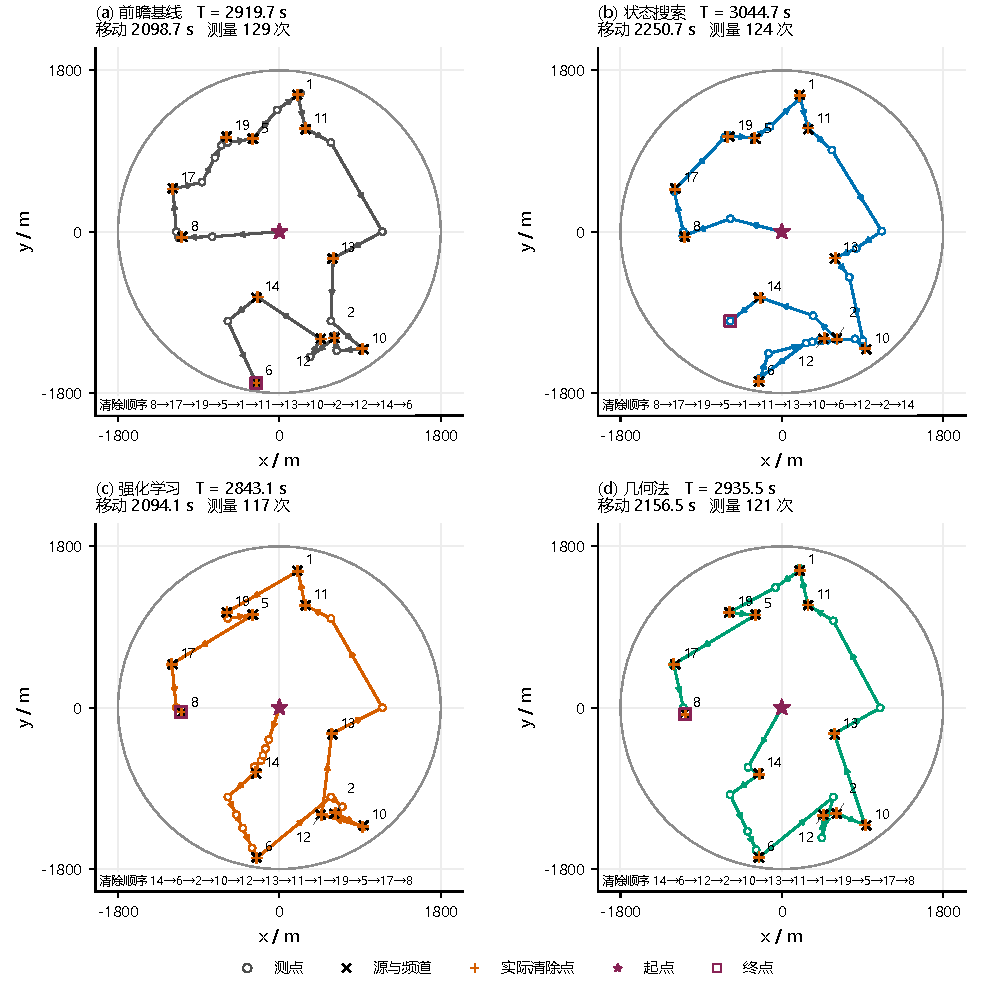
\includegraphics[width=\linewidth,height=\textheight,keepaspectratio,alt={状态搜索最大退化场景800015。状态搜索虽减少检测，却因移动增长而较基线慢125.08 s；此例为事后诊断选择。}]{figures/fig07_trajectory_state_worst.pdf}
\caption{状态搜索最大退化场景800015。状态搜索虽减少检测，却因移动增长而较基线慢125.08 s；此例为事后诊断选择。}
\label{fig:q23-7}
\end{figure}

\begin{figure}[!htbp]
\centering
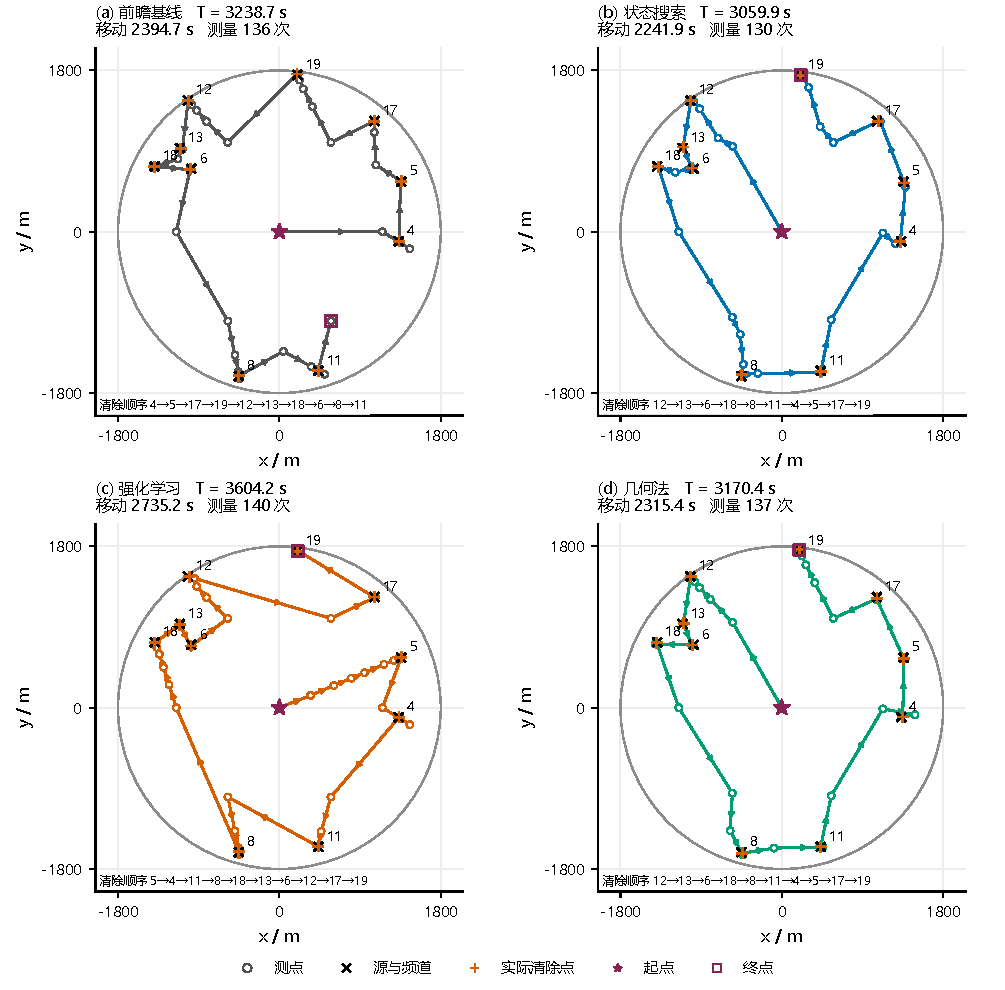
\includegraphics[width=\linewidth,height=\textheight,keepaspectratio,alt={PPO最大退化场景800081。该例主要额外代价来自移动，PPO较基线慢365.45 s；此例不表示总体发生频率。}]{figures/fig08_trajectory_rl_worst.pdf}
\caption{PPO最大退化场景800081。该例主要额外代价来自移动，PPO较基线慢365.45 s；此例不表示总体发生频率。}
\label{fig:q23-8}
\end{figure}

\FloatBarrier

%
\end{document}
